\documentclass[11pt,oneside]{article}    %use"amsart"insteadof"article"forAMSLaTeXformat
\usepackage{geometry}        %Seegeometry.pdftolearnthelayoutoptions.Therearelots.
\geometry{letterpaper}        %...ora4paperora5paperor...
%\geometry{landscape}        %Activateforforrotatedpagegeometry
%\usepackage[parfill]{parskip}        %Activatetobeginparagraphswithanemptylineratherthananindent
\usepackage{graphicx}                %Usepdf,png,jpg,orepsßwithpdflatex;useepsinDVImode
                                %TeXwillautomaticallyconverteps-->pdfinpdflatex        
\usepackage{amssymb}
\usepackage[colorlinks]{hyperref}
\usepackage{commath}

%----macros begin---------------------------------------------------------------
\usepackage{color}
\usepackage{amsthm}

\def\conv{\mbox{\textrm{conv}\,}}
\def\aff{\mbox{\textrm{aff}\,}}
\def\E{\mathbb{E}}
\def\R{\mathbb{R}}
\def\Z{\mathbb{Z}}
\def\tex{\TeX}
\def\latex{\LaTeX}
\def\v#1{{\bf #1}}
\def\p#1{{\bf #1}}
\def\T#1{{\bf #1}}

\def\vet#1{{\left(\begin{array}{cccccccccccccccccccc}#1\end{array}\right)}}
\def\mat#1{{\left(\begin{array}{cccccccccccccccccccc}#1\end{array}\right)}}

\def\lin{\mbox{\rm lin}\,}
\def\aff{\mbox{\rm aff}\,}
\def\pos{\mbox{\rm pos}\,}
\def\cone{\mbox{\rm cone}\,}
\def\conv{\mbox{\rm conv}\,}
\newcommand{\homog}[0]{\mbox{\rm homog}\,}
\newcommand{\relint}[0]{\mbox{\rm relint}\,}

%----macros end-----------------------------------------------------------------

\newtheorem{definition}{Definition}
\newtheorem{statement}{Statement}

\title{Triangulation of the boundary of a 2-chain
\footnote{This document is part of the \emph{Linear Algebraic Representation with CoChains} (LAR-CC) framework~\cite{cclar-proj:2013:00}. \today}
}
\author{Alberto Paoluzzi}
%\date{}                            %Activatetodisplayagivendateornodate

\begin{document}
\maketitle
\nonstopmode

\begin{abstract}
In this module we perform the whole set of manipulations necessary to triangulate the boundary polygon of a 2-chain using a standard triangulation algorithm~\cite{} implemented by the \texttt{poly2tri} python package, largely diffuse in games applications.
Notice that the input data may be of very general kind, corresponding to polygons that are non-connected, non-manifold w/o nested polygons of general kind. Conversely, the used library allows only for quite special polygons, with a simple exterior boundary and multiple (non-touching) internal holes, and without repeated vertices. The used package is based on the paper "Sweep-line algorithm for constrained Delaunay triangulation" by V.~Domiter and B.~Zalik~\cite{poly2tri:2008}.
\end{abstract}

\tableofcontents


\section{From a finite set of 2D segments to a regular 2-complex}
%===============================================================================

Let suppose that a  2-complex in the plane is given as a LAR triple \texttt{(V,FV,EV)}, and that a 2-chain $\texttt{chain}\in\Z_2^n$ is also given, with $\Z_2=\{0,1\}$ and $n = |\texttt{V}|$.
The aim of this module is to develop a methodology and an implementation to compute a triangulation of any 2-chain extracted from a 2-complex. 

This first section will concentrate on (1) how to generate a regular 2-complex starting from a finite set of 2D segments, i.e.~how to generate a LAR triple \texttt{(V,FV,EV)},  and (2)~how to triangulate \emph{any 2-chain}, and in particular a single 2-cell in 2D, using a standard CDT  (Constrained Delaunay Triangulation) algorithm that does not allow for polygons with repeated vertices. 

The first point is not trivial, since a general 2-chain may contain 2-cells that are not contractible to a point (since they may contain any finite number of internal holes), and furthermore may be non-manifold, i.e.~with boundary vertices incident on more than 2 boundary edges. In addition, in the general case, holes of 2-cells may contain other 2-cells, possibly with holes, and so on. 

In particular, the presence of non-manifold vertices is the common case in random generation of complexes of polygons in the plane, and/or for the typical 2-chain extracted from a general 2-complex. In order of preparing the input for the triangulation algorithm, the boundary 0-chain extracted from the general 2-chain must undergo to a  circular ordering, producing---in the non-manifold case---any finite number of vertex repetitions. Repeated vertices will be disambiguated by applying small local perturbations towards the interior of the cycle. Anyway, boundary cycles will be perturbed only for drawing solidly the 2-chain as a single polygon with holes, whereas the exact LAR of the 2-complex will not be modified.

\subsection{Definitions and methodology}

First we provide some definitions useful in what follows, then we formalize the implemented methods.

\begin{definition}{(Regular complex)}
A $d$-complex is \emph{regular} when any $k$-cell ($0 \leq k \leq d$) is contained in a $d$-cell.
\end{definition}

\begin{definition}{(Circular ordering)}
A $0$-chain is \emph{circularly ordered} when every consecutive pair of its $0$-cells (module the lenght of the chain) maps to a $1$-cell of the boundary 1-chain of a 2-chain.
\end{definition}



\subsubsection{Input preprocessing}

The input is given by $m$ line segments in the plane, with $p\leq 2m$ extreme points.

First we compute all the $k$ intersection points internal to the lines, using adeguate data structures and algorithms to accelerate the search. This problem is developed within the \texttt{inters} module, and implemented in the \texttt{larlib} sub-package named \texttt{inters.py}. 

The arrangement of lines is correspondingly updated---by splitting the input lines on their \emph{internal} intersection points---so that the splitted line segments may possibly intersect only on extreme points.

Let consider the undirected graph $G=(N,A)$, where the set of nodes $N$ is given by the extreme points of splitted  segments, and compute the set  $\mathcal{G} = \{G_i\}_{i\in I}$ of maximal biconnected components of $G$.    Suppose $\mathcal{G}$ nonempty.

\begin{definition}{(Vertices)}
The union of node sets of biconnected components provides the \emph{vertex} set $\texttt{V} = \cup_{i\in I} N_i$.
This one supplies the geometric embedding of the 0-cells of the 2-complex.
\end{definition}

\begin{definition}{(Edges)}
The disjoint union of arcs of biconnected components provides the \emph{edge set} $\texttt{EV} = \cup_{i\in I} A_i$.
It supplies an indexed array of pairs of node indices, i.e.~a LAR representation of the 1-cells of the 2-complex.
\end{definition}


\begin{definition}{(Cycles)}
The \emph{boundaries} of 2-chains, corresponding one-to-one to the biconnected components $G_i \in \mathcal{G}$ considered as a plane partition, are \emph{closed} 1-chains called \emph{cicles} $\mathcal{C} = \{\partial G_i\}_{i\in I}$.
\end{definition}

A cycle may be represented either as an unordered set of 1-cells (1-chain) or as an ordered set of 0-cells (0-chain), that we call \emph{1-cycle} and \emph{0-cycle}, respectively.

\begin{definition}{(Manifold and non-manifold cycles)}
A boundary 1-chain with a number $n$ of both 1-cells and 0-cells may be represented as a permutation of vertex indices. We call it a \emph{manifold cycle}.  Conversely, if the number of its vertices is smaller than the number of its edges, then the cycle is a \emph{non-manifold}.
\end{definition}

A cycle may be decomposed into one or more loops of edges. In a cycle all loops are piecewise-linear curves; they share one or more common vertices in the case of non-manifold cycles. The set of loops, denoted in the following as $\mathcal{L}$, has cardinality $\ell = |\mathcal{L}|$ greater or equal to the cardinality $n = |\mathcal{G}|$, where the non-manifold vertices have even incidence number greater than 2.
The cycles in $\mathcal{C}$ are boundaries of connected regions of the plane. The loops in $\mathcal{L}$ are boundaries of regions contractible to a point. 


\subsubsection{Algorithm: LAR generation}
\label{sec:larFromCycles}

Every cycle in $\mathcal{C}$ subdivides the plane in 3 regions, of internal, external, and boundary points, respectively. The set union of $\mathcal{C}$ elements provides a \emph{cover} of the plane. Let us consider the collection $\mathring{\mathcal{C}}$ of the open sets of points internal to the cycles.

\begin{definition}{(Faces)}
A partition of the plane is given by the collection of closures of the set differences (\emph{regularized differences}) between every element of $\mathring{\mathcal{C}}$ and all the others. We call this set \texttt{F}, and its elements either \emph{faces} or 2-cells of the 2-complex.
\end{definition}

The triple \texttt{(V,E,F)}, as defined before, is a cellular 2-complex defined by the $d$-cells ($0\leq d\leq 2$) in \texttt{V,E,F}, that provide the 0-, 1-, and 2-cells, respectively. 

\begin{statement}{(LAR)}
Every cell of a 2-complex as a collection of point-sets is completely is represented discretely, in the sense that can be completely reconstructed, starting from the \texttt{V} subset of its boundary.
\end{statement}

The point now is how to construct the array \texttt{FV} starting from the arrays \texttt{V}, \texttt{EV}, and from the set $\mathcal{C}$ returned by the function \texttt{farFromLines()} implemented in the \texttt{larlib} module \texttt{inters.py}.

\begin{figure}[htbp] %  figure placement: here, top, bottom, or page
   \centering
   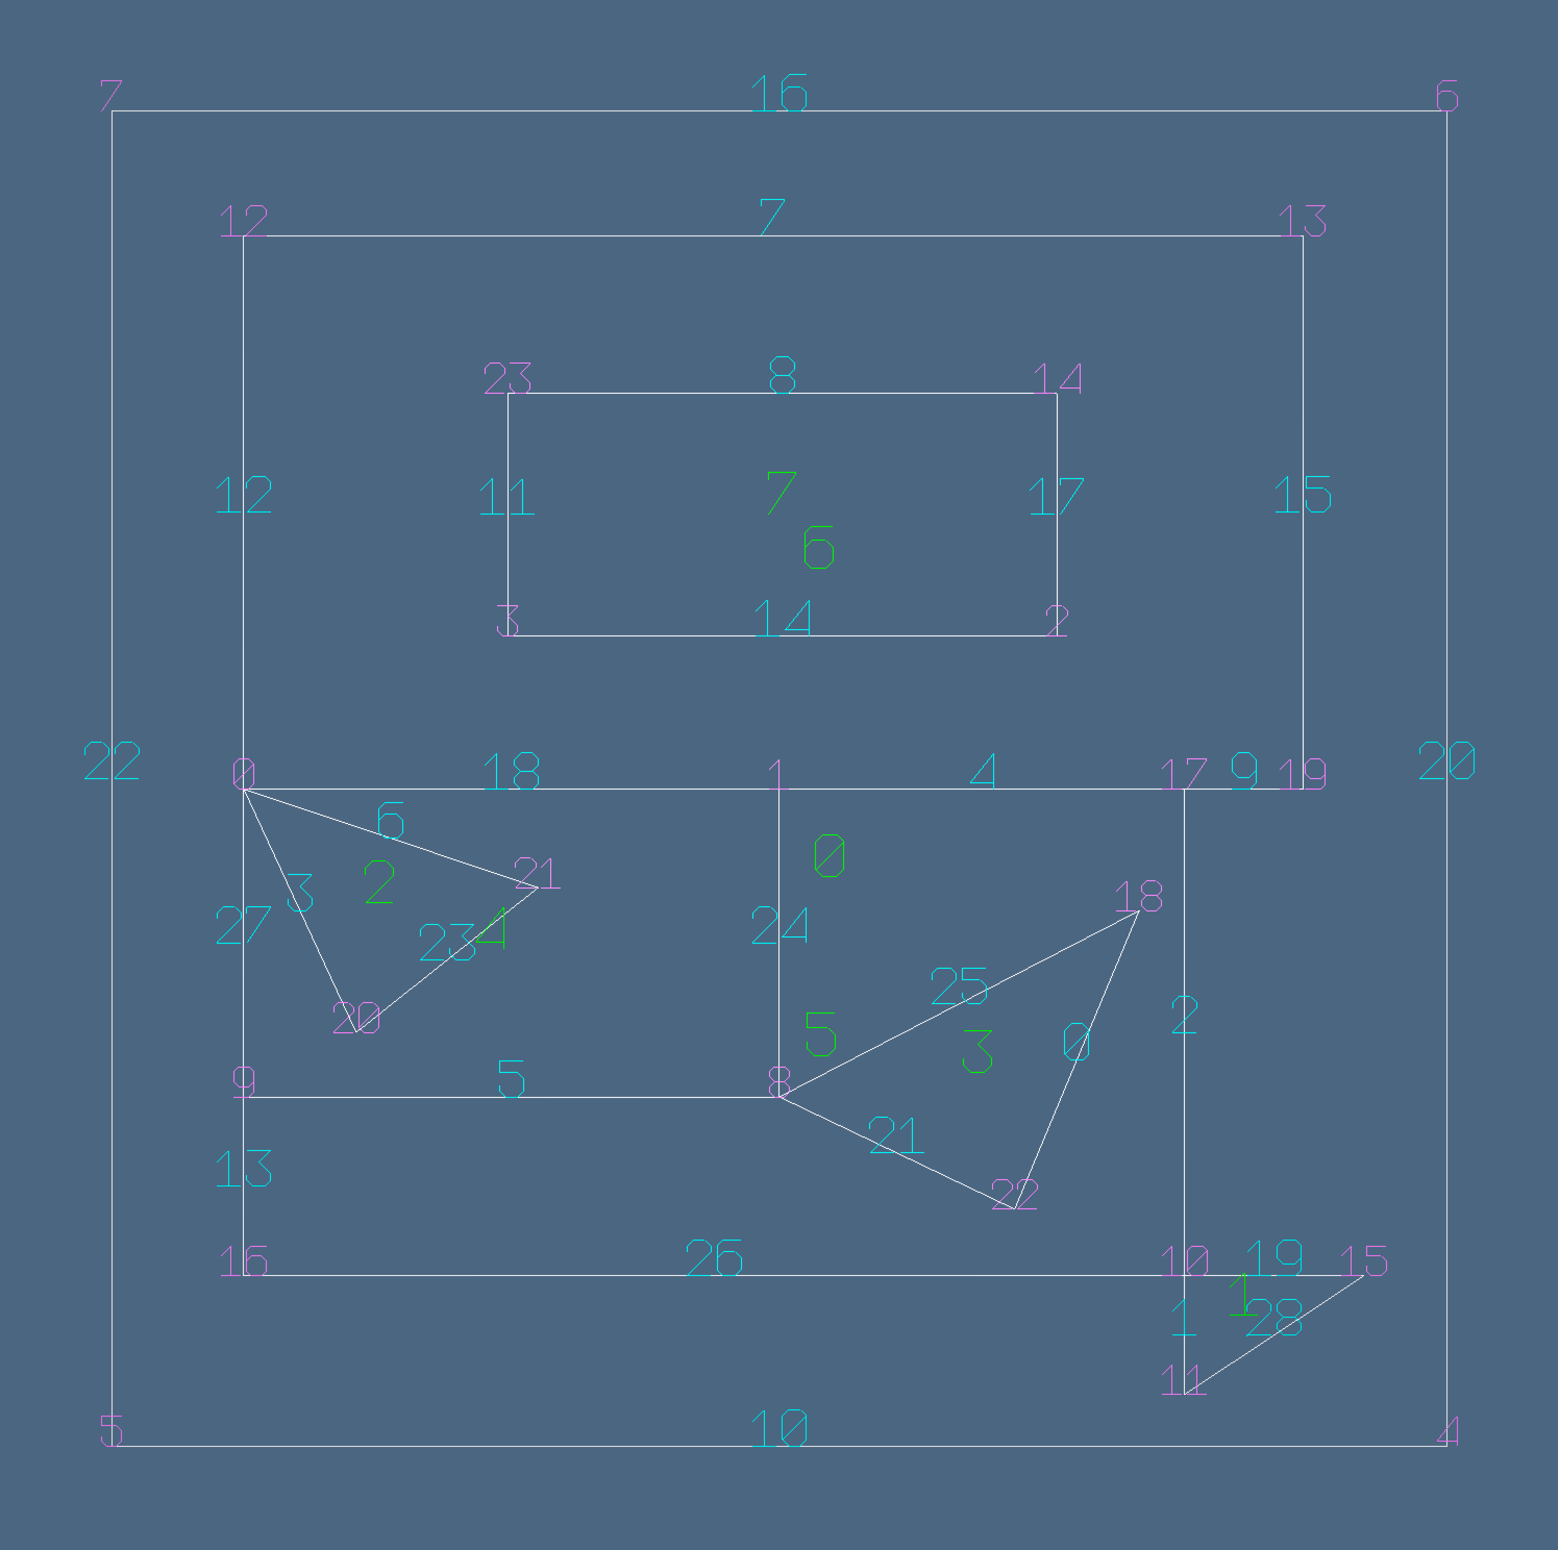
\includegraphics[width=0.328\linewidth]{images/linesToLAR0} 
   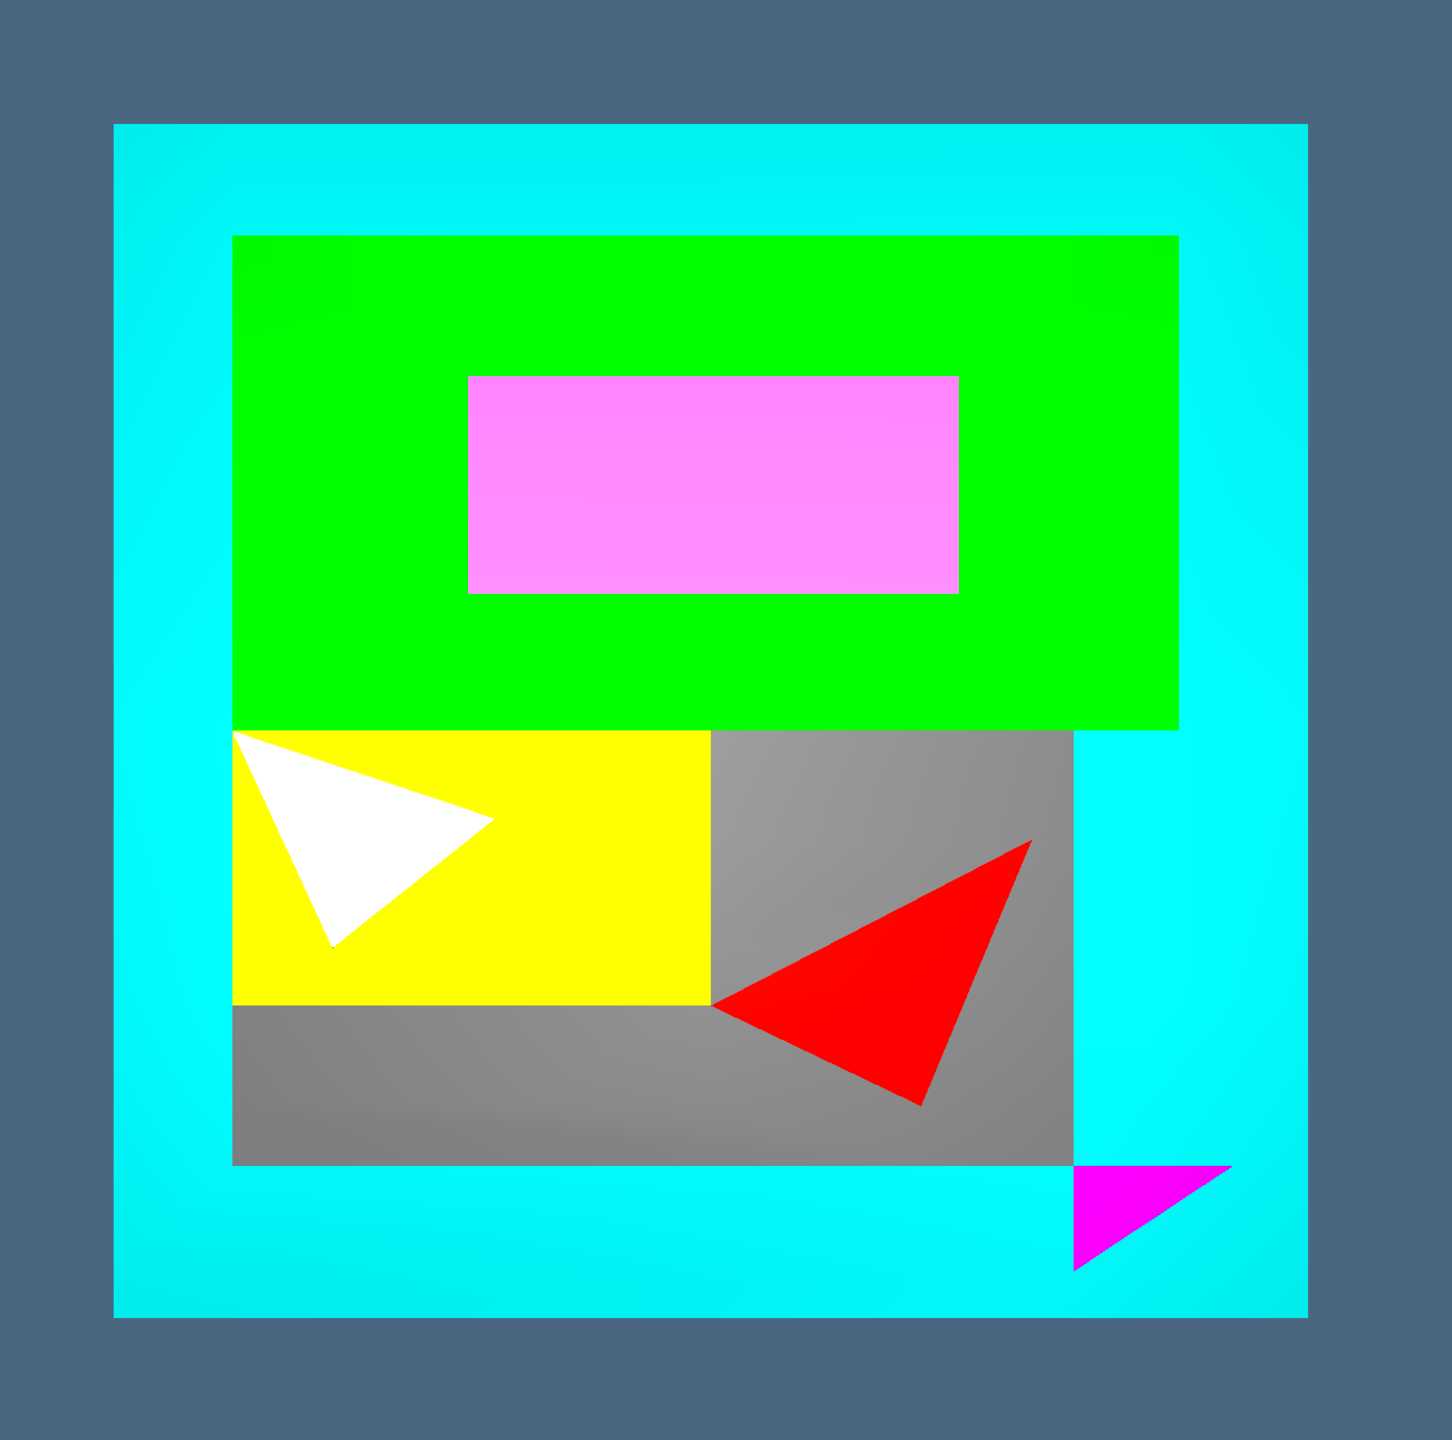
\includegraphics[width=0.3285\linewidth]{images/linesToLAR1} 
   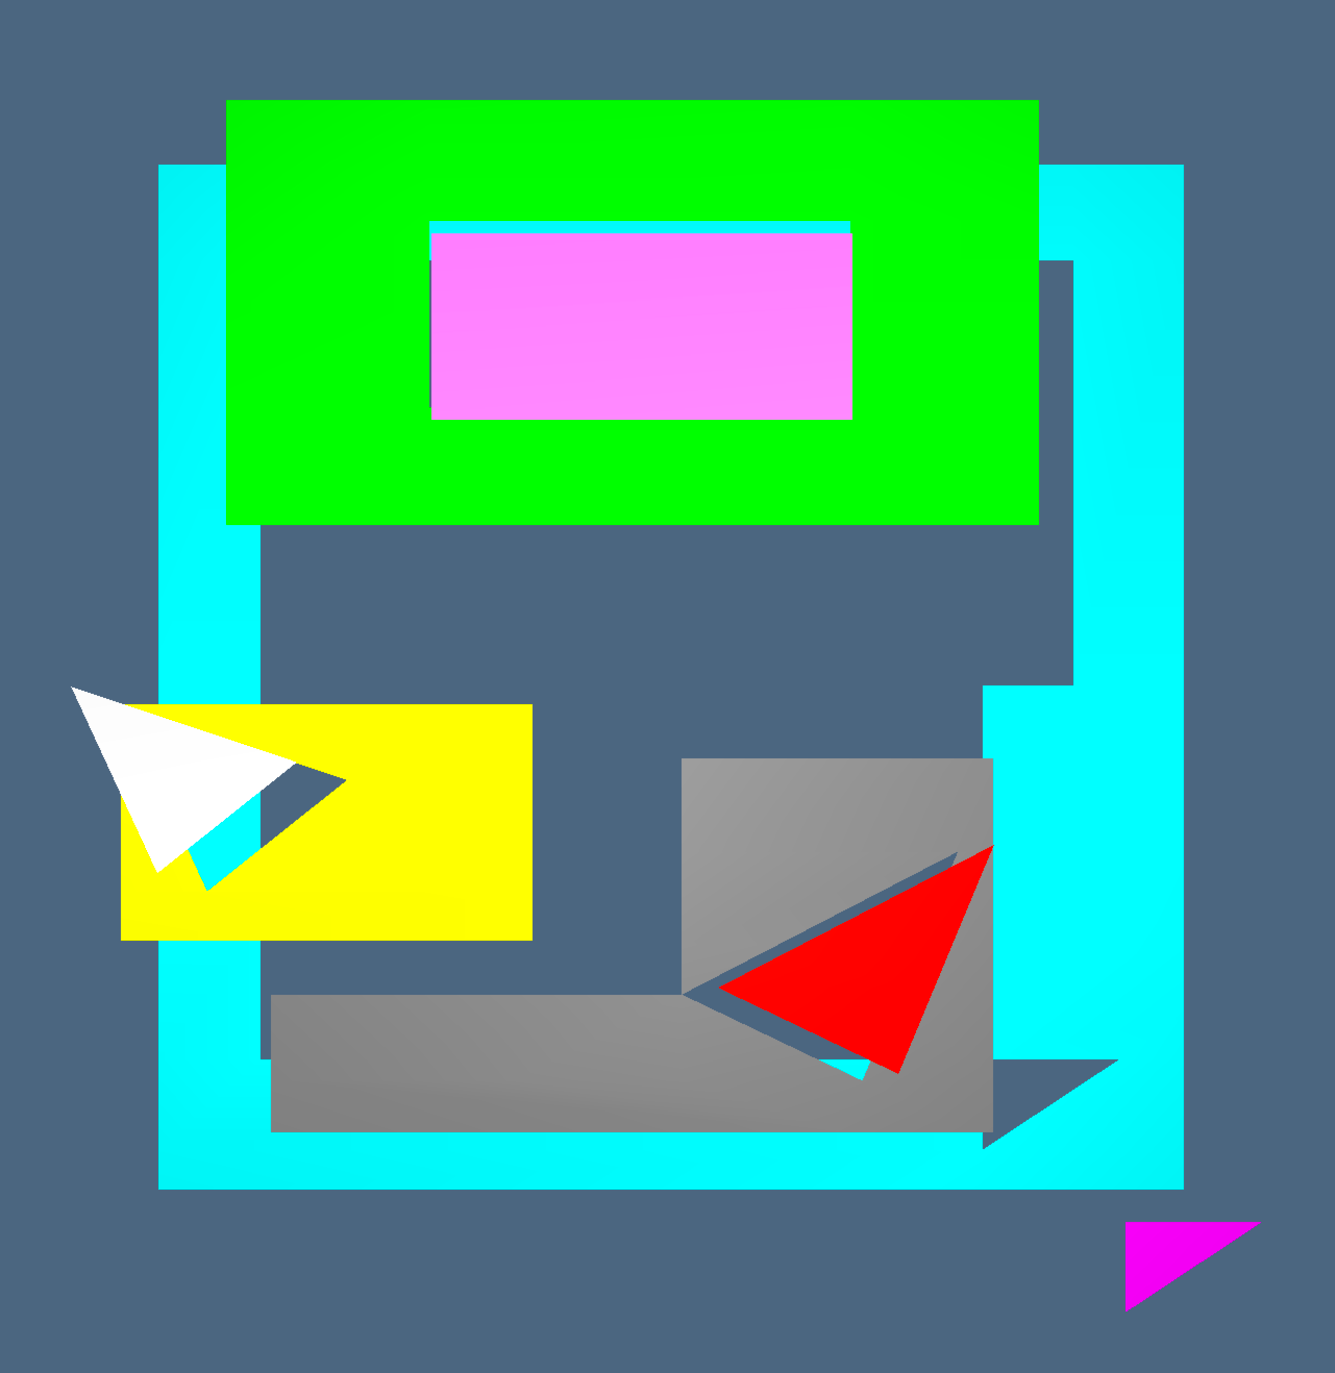
\includegraphics[width=0.321\linewidth]{images/linesToLAR2} 
   \caption{LAR cellular 2-complex generated by an arrangement of line segments: (a) drawing of numbered cells; (b) 2-complex with different colors; (c) exploded view of 2-cells. Notice that every cell is connected, but not necessarily  path-connected.}
   \label{fig:linesToLAR}
\end{figure}


\paragraph{Computing a LAR 2-complex from an arrangement of line segments}

The computational process discussed in Section~\ref{sec:larFromCycles} is implemented by the script below.
First, the planar graph of edges is built by the \texttt{lines2lar} function, then the set of graph \texttt{cycles} corresponding to the partition of 2D plane induced by the graph is returned by the \texttt{facesFromComps} function. These are sorted in increasing order of the surrounded area, so getting at the end of the sorted list two copies of the exterior boundary cycle. The very last cycle is removed, so that every internal edge is used twice in some cycle, whereas the boundary edges are used only once. Finally the various cycles are checked pairwise for mutual containment, producing the \texttt{latticeArray} of their partial order.
Finally, the reduced set of \texttt{cells} as lists of bounding cycles of vertices is produced by the \texttt{cellsFromCycles} function, finally removed by multiple vertices to produce the \texttt{FV} LAR representation.

%-------------------------------------------------------------------------------
@D Computing a LAR 2-complex from an arrangement of line segments
@{""" Computing a LAR 2-complex from an arrangement of line segments"""
def larPair2Triple(model):
    V,EV = model
    cycles,ecycles = makeCycles(model)
    print "\necycles =",ecycles,"\n"
    areas = AA(ABS)(integr.surfIntegration((V,cycles,EV),True))
    orderedCycles = sorted([[area,cycles[f]] for f,area in enumerate(areas)])
    interiorCycles = [face for area,face in orderedCycles[:-1]]
    EdgeCyclesByVertices = [zip(cycle[:-1],cycle[1:])+[(cycle[-1],cycle[0])] 
                                for cycle in interiorCycles]
    latticeArray = computeCycleLattice(V,EdgeCyclesByVertices)
    cells = cellsFromCycles(latticeArray)
    polygons = [[interiorCycles[k] for k in cell] for cell in cells]
    return V,polygons,EV
@}
%-------------------------------------------------------------------------------



\paragraph{LAR of a 2-complex of general type}

The LAR of the complex in Figure~\ref{fig:linesToLAR}, and constructed starting from a set of line segmants in the plane, is given here. Notice that cells may have non connected boundaries (may contain holes) and/or non-manifold points.

%-------------------------------------------------------------------------------
@O test/py/triangulation/test08.py
@{""" Test example of LAR of a 2-complex with non-contractible and non-manifold cells"""
from larlib import *

V = [[0.0989,0.492],[0.5,0.492],[0.708,0.6068],[0.2966,0.6068],[1.0,0.0], 
[0.0,0.0],[1.0,1.0],[0.0,1.0],[0.5,0.2614],[0.0989,0.2614],[0.8034,
0.1273],[0.8034,0.0386],[0.0989,0.9068],[0.892,0.9068],[0.708,0.7886],
[0.9375,0.1273],[0.0989,0.1273],[0.8034,0.492],[0.7693,0.4009],[0.892,
0.492],[0.183,0.3097],[0.3193,0.4182],[0.6761,0.1773],[0.2966,0.7886]]

FV = [[0,4,5,6,7,9,10,11,12,13,15,16,17,19],[10,11,15],[0,20,21],[8,18,
22], [0,1,8,9,20,21],[1,8,9,10,16,17,18,22],[0,1,2,3,12,13,14,17,19,23],
[2,3,14,23]]

EV = [(18,22),(10,11),(10,17),(0,20),(1,17),(8,9),(0,21),(12,13),(14,23), 
(17,19),(4,5),(3,23),(0,12),(9,16),(2,3),(13,19),(6,7),(2,14),(0,1),
(10,15),(4,6),(8,22),(5,7),(20,21),(1,8),(8,18),(10,16),(0,9),(11,15)]

VV = AA(LIST)(range(len(V)))
submodel = STRUCT(MKPOLS((V,EV)))        
VIEW(larModelNumbering(1,1,1)(V,[VV,EV,FV],submodel,0.3)) 
@}
%-------------------------------------------------------------------------------


\paragraph{Generation of LAR of a 2-complex from line segments}
The LAR model \texttt{(V,FV,EV)} displayed in Figure~fig:linesToLAR and listed in the Script above, 
i.e.~ in the \texttt{test08.py} file, can be generated as below.
%-------------------------------------------------------------------------------
@O test/py/triangulation/test09.py
@{""" Test example of LAR of a 2-complex with non-contractible and non-manifold cells"""
from larlib import *

filename = "test/svg/inters/test0.svg"
lines = inters.svg2lines(filename)
V,FV,EV,polygons = larFromLines(lines)

VV = AA(LIST)(range(len(V)))
hpc = STRUCT(MKPOLS((V,EV)))        
VIEW(larModelNumbering(1,1,1)(V,[VV,EV,FV],hpc,0.2)) 
@}
%-------------------------------------------------------------------------------

%-------------------------------------------------------------------------------
@O test/py/triangulation/test11.py
@{""" Test example of LAR of a 2-complex with non-contractible and non-manifold cells"""
from larlib import *

filename = "test/svg/triangulation/facade.svg"
lines = inters.svg2lines(filename)
V,FV,EV,polygons = larFromLines(lines)

VV = AA(LIST)(range(len(V)))
hpc = STRUCT(MKPOLS((V,EV)))        
VIEW(larModelNumbering(1,1,1)(V,[VV,EV,FV],hpc,0.2)) 
@}
%-------------------------------------------------------------------------------


\paragraph{Solid PyPLaSM visualization of a 2-complex}

A PyPLaSM visualization of a 2-complex of very general kind may be obtained with the \texttt{MKFACES} function, implemented by the \texttt{SOLIDIFY} of geometric values of \emph{HPC} type, starting from the LAR model of the 2-complex to be displayed. Of course, a \texttt{boundaryOperator} is built using the LAR representation of 2-cells and 1-cells, i.e.~\texttt{FV} and \texttt{EV}, respectively.

In order to make the function applicable also to embedded 2-complexes (notice that for our purposes it mekes sense to embed only in 3D), an affine transformation and its inverse must be applied to each face in order to \texttt{SOLIDIFY} it.

%-------------------------------------------------------------------------------
@D Solid PyPLaSM visualization of a 2-complex
@{""" Solid PyPLaSM visualization of a 2-complex with non-contractible 
      and non-manifold cells"""
import bool
def MKFACES(model):
    V,FV,EV = model
    VV = AA(LIST)(range(len(V)))
    bmatrix = boundary1(FV,EV,VV)
    boundaryOperator = chain2BoundaryChain(bmatrix)
    chain = [0]*len(FV)
    boundingEdges = []
    for k,face in enumerate(FV):
        unitChain = copy.copy(chain)
        unitChain[k] = 1
        boundingEdges += [boundaryOperator(unitChain)]
    print "boundingEdges =",boundingEdges
    if len(V[0])==3:
        faces = []
        for faceEdges in boundingEdges:
            facet = [V[v] for e in faceEdges for v in EV[e]]
            transformMat = bool.faceTransformations(array(facet))
            verts = (transformMat*mat(facet).T).T.tolist()
            z = verts[0][-1]
            verts2D = [vert[:-1] for vert in verts]
            polylines = [POLYLINE([verts2D[k],verts2D[k+1]]) for k in range(0,len(verts2D),2)]
            hpc = SOLIDIFY(STRUCT(polylines))
            verts2D,cells,pols = UKPOL(hpc)
            verts3D = mat([v+[z] for v in verts2D]).T
            verts3D = (transformMat.I*verts3D).T         
            faces += [MKPOL([verts3D.tolist(),cells,pols])]
    elif len(V[0])==2:
        faces = [SOLIDIFY(STRUCT([POLYLINE([V[v] for v in EV[e]]) for e in edges])) 
            for edges in boundingEdges]
    return faces
@}
%-------------------------------------------------------------------------------


\paragraph{Color visualization}
A color visualization of the 2-cells of the previous cellular complex is produced by the \texttt{test10.py} file, using the HPC visualization based on Pyplasm XOR.

%-------------------------------------------------------------------------------
@O test/py/triangulation/test10.py
@{""" Test example of LAR of a 2-complex with non-contractible and non-manifold cells"""
from larlib import *
sys.path.insert(0, 'test/py/triangulation/')
from test09 import *

model = V,FV,EV

faces = MKFACES(model)
colors = [CYAN,MAGENTA,WHITE,RED,YELLOW,GRAY,GREEN,ORANGE,BLUE,PURPLE,BROWN,BLACK]
components = [COLOR(colors[k%12])(faces[k]) for k in range(len(FV))]
VIEW(STRUCT(components))
@}
%-------------------------------------------------------------------------------
%-------------------------------------------------------------------------------
@O test/py/triangulation/test12.py
@{""" Test example of LAR of a 2-complex with non-contractible and non-manifold cells"""
from larlib import *
sys.path.insert(0, 'test/py/triangulation/')
from test11 import *

model = V,FV,EV

faces = MKFACES(model)
colors = [CYAN,MAGENTA,WHITE,RED,YELLOW,GRAY,GREEN,ORANGE,BLUE,PURPLE,BROWN,BLACK]
components = [COLOR(colors[k%12])(faces[k]) for k in range(len(FV))]
VIEW(STRUCT(components))

VIEW(STRUCT(MKFACES((V,[FV[4]],EV))))
@}
%-------------------------------------------------------------------------------

\begin{figure}[htbp] %  figure placement: here, top, bottom, or page
   \centering

   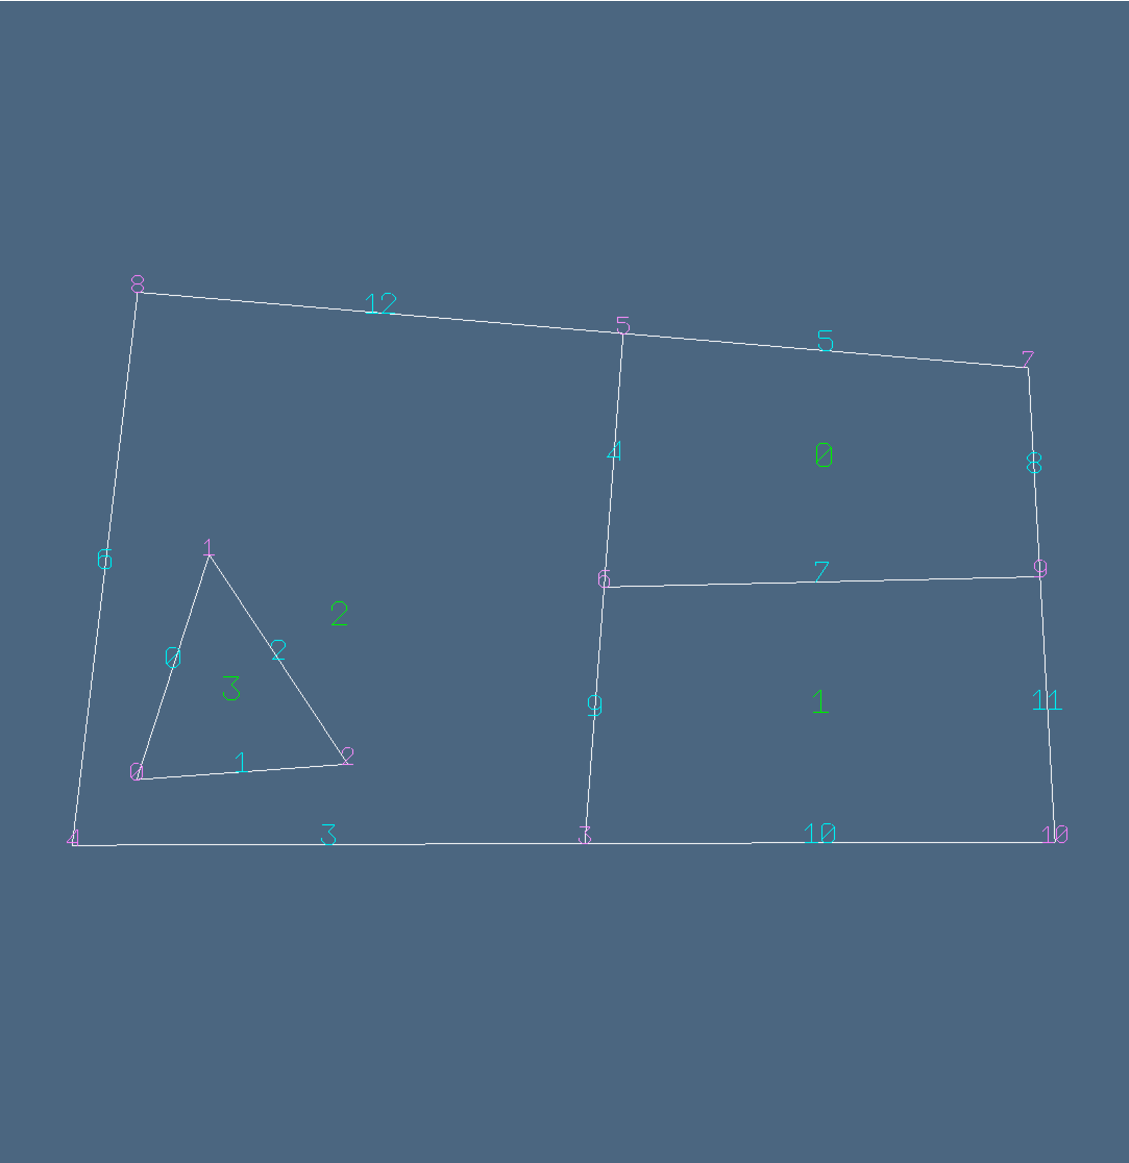
\includegraphics[height=0.325\linewidth,width=0.325\linewidth]{images/grapha} 
   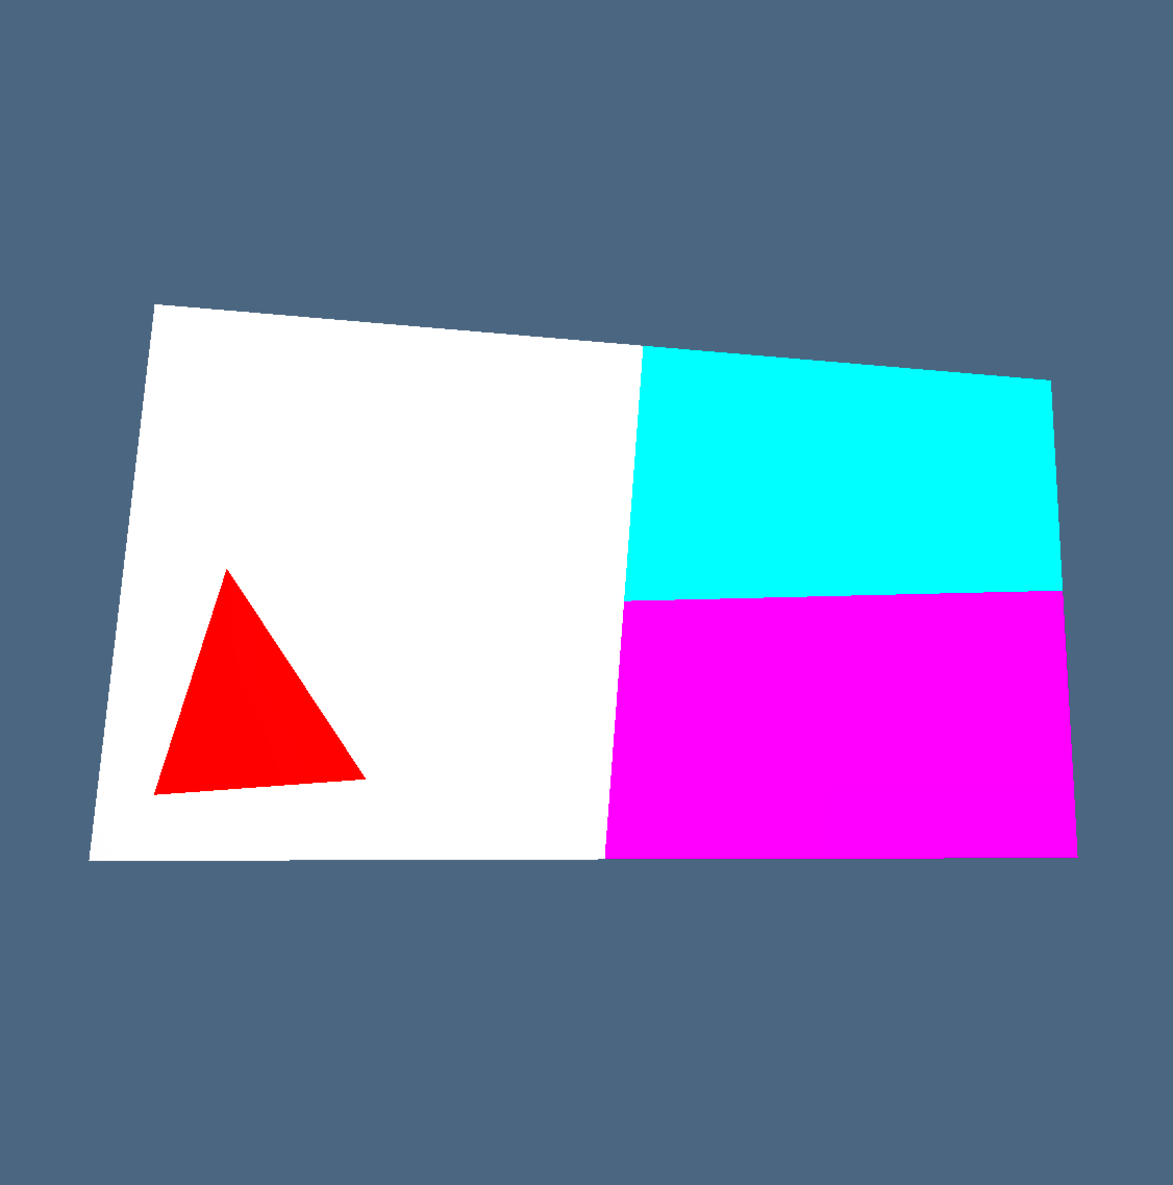
\includegraphics[height=0.325\linewidth,width=0.325\linewidth]{images/graphb} 
   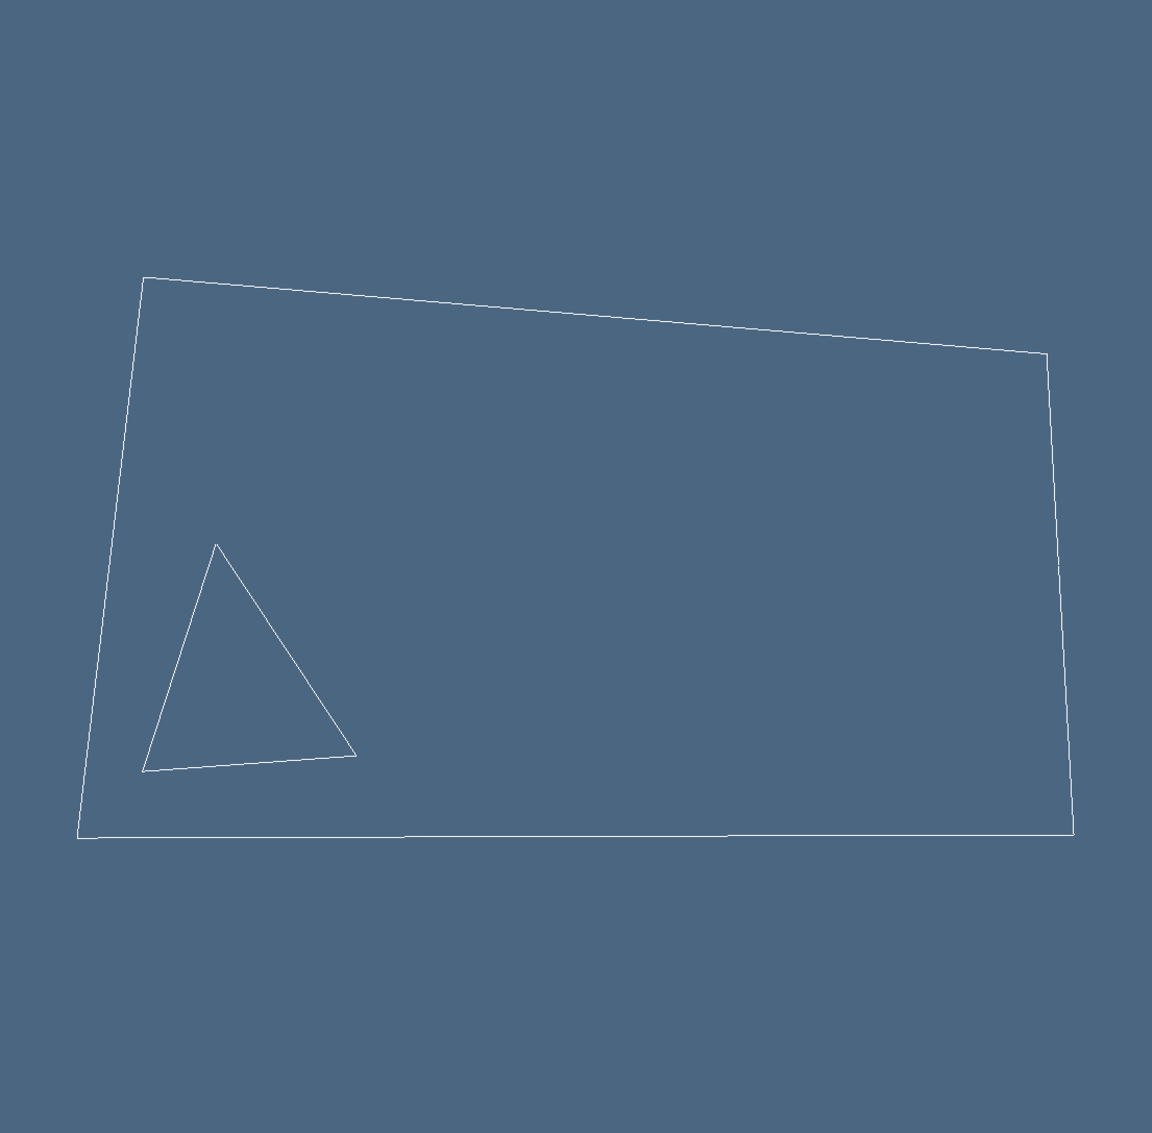
\includegraphics[height=0.325\linewidth,width=0.325\linewidth]{images/graphc} 

   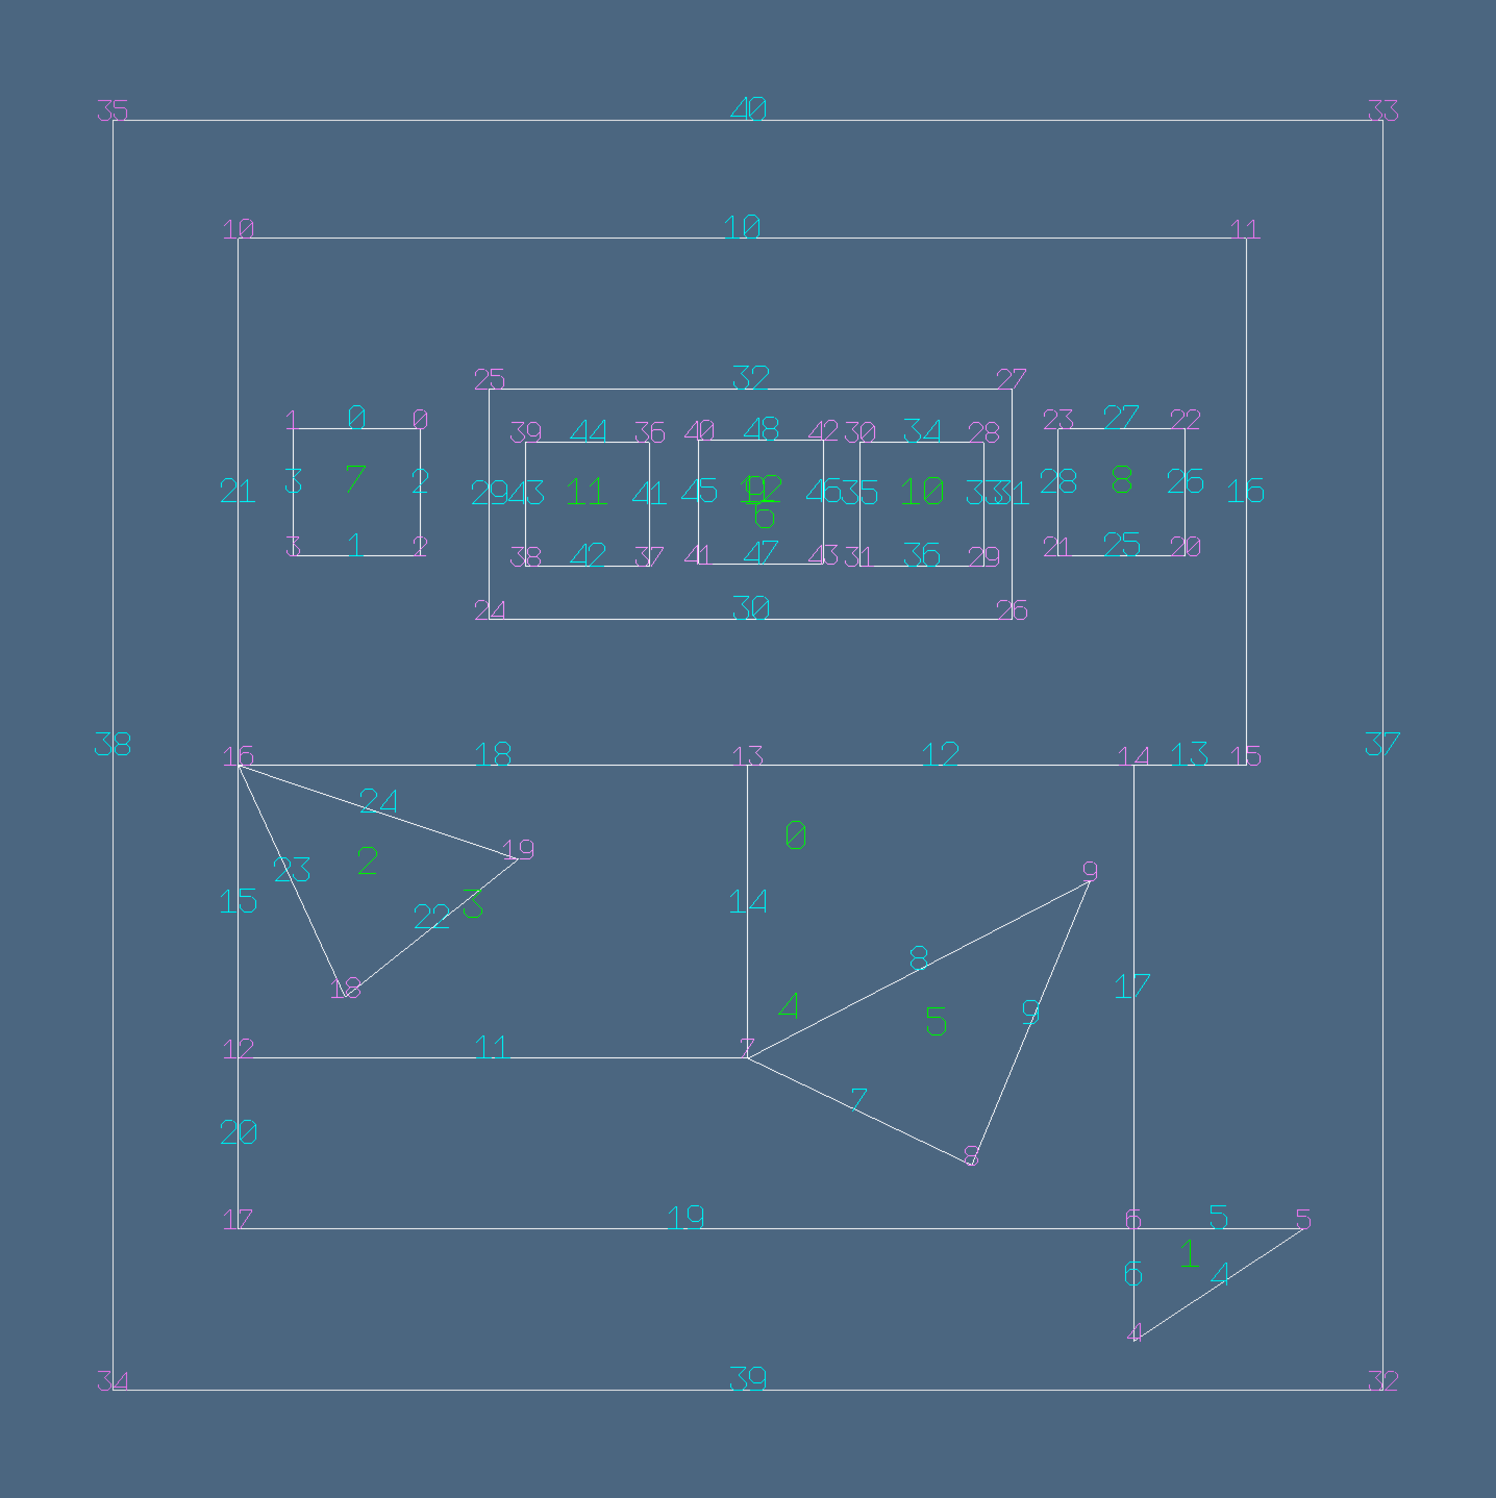
\includegraphics[width=0.325\linewidth]{images/test0a} 
   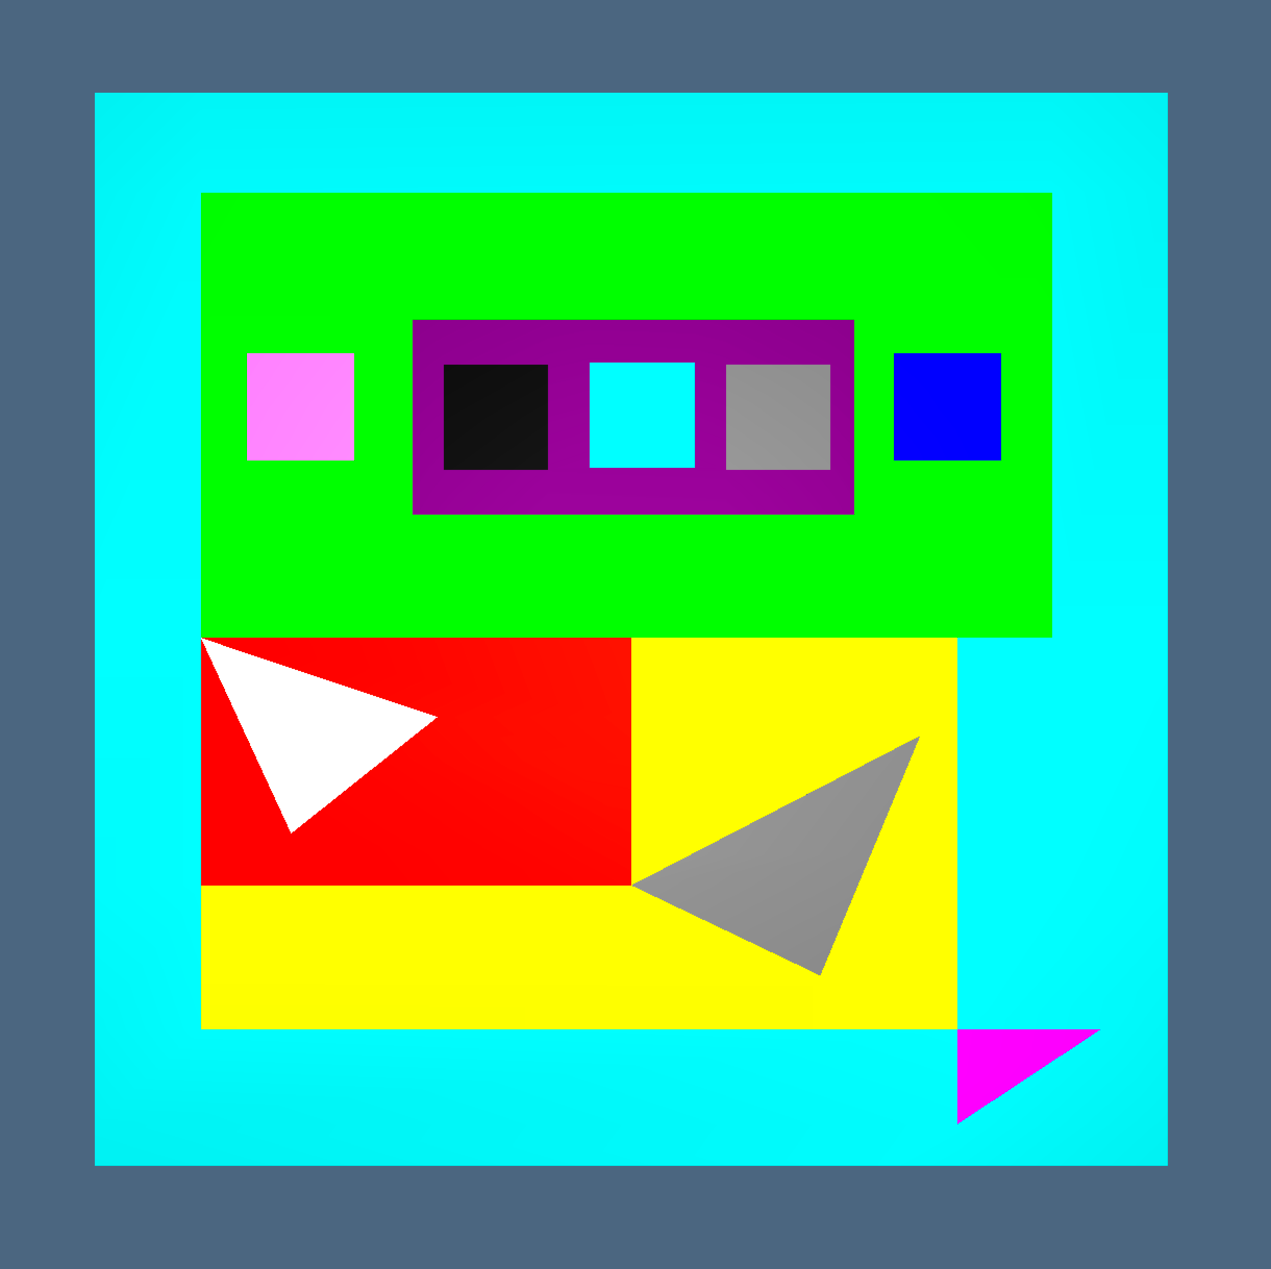
\includegraphics[width=0.325\linewidth]{images/test0b} 
   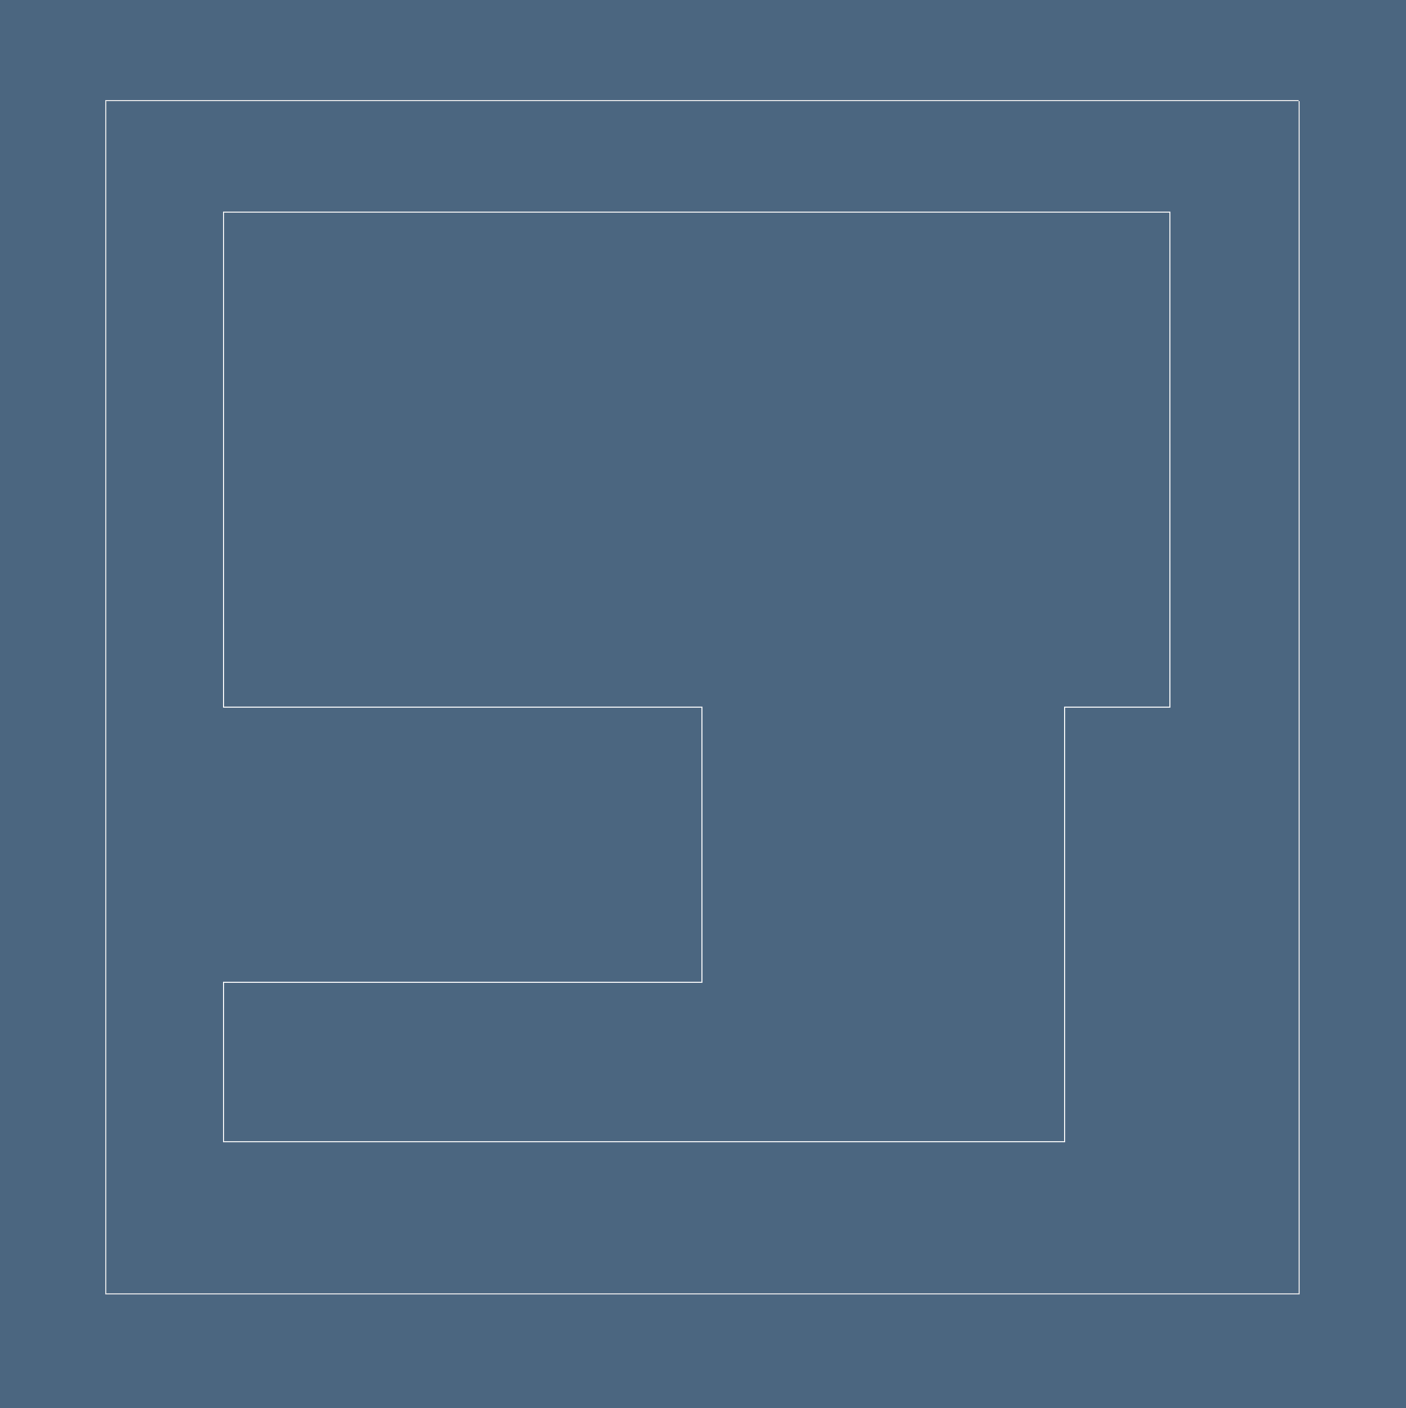
\includegraphics[width=0.325\linewidth]{images/test0c} 

   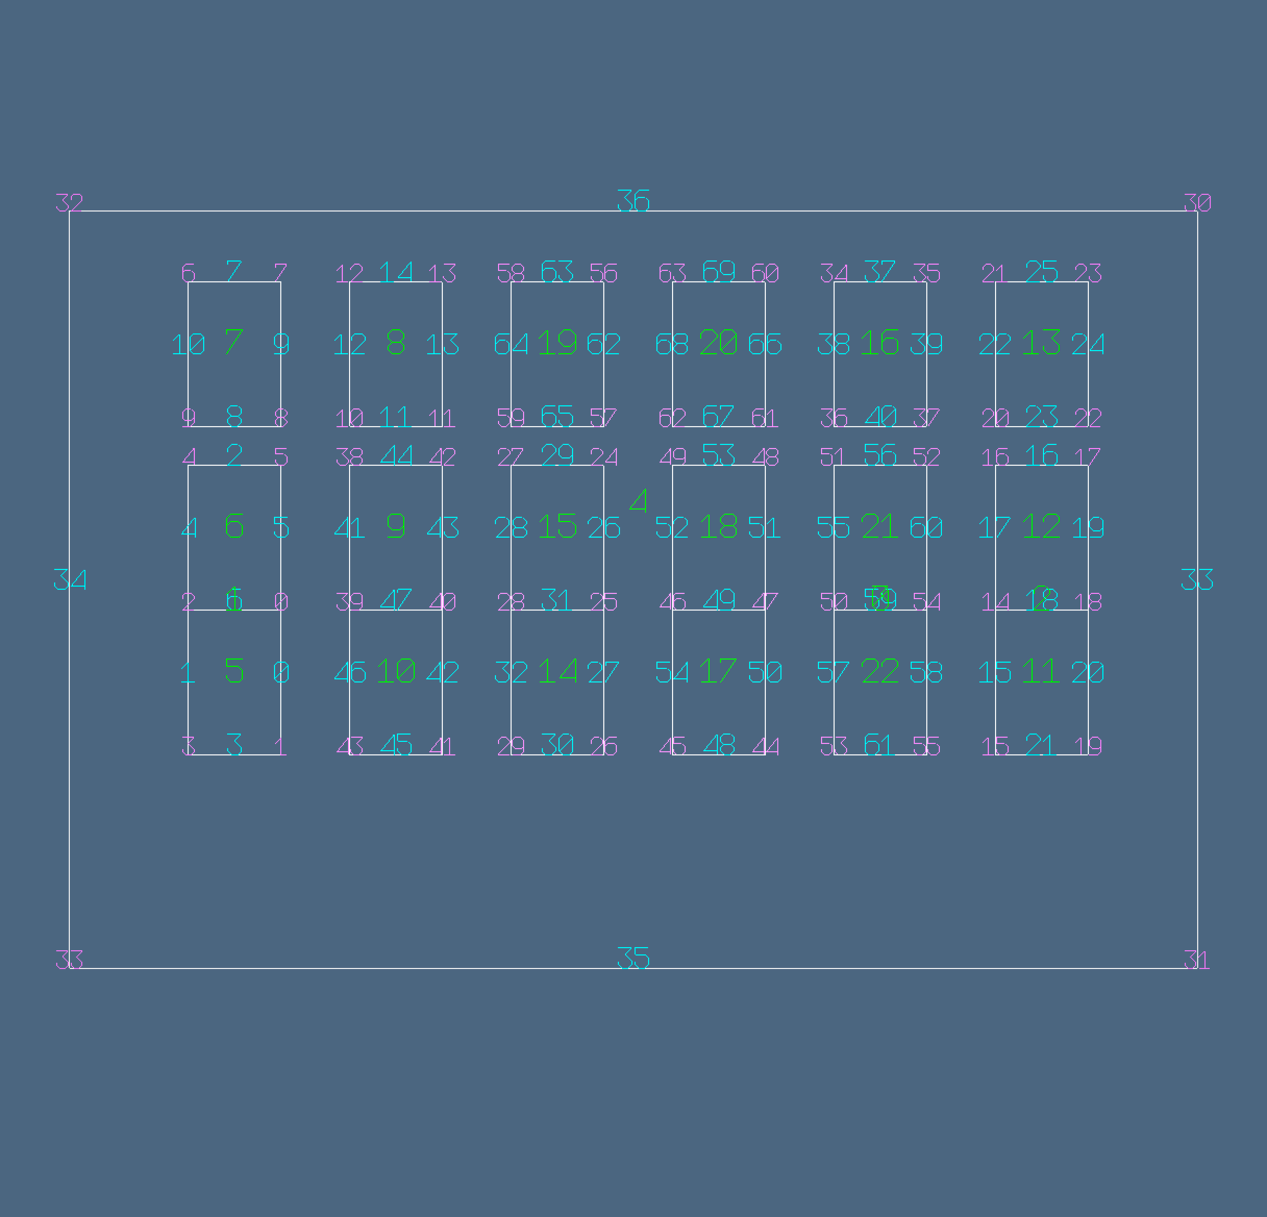
\includegraphics[height=0.325\linewidth,width=0.325\linewidth]{images/facade-a} 
   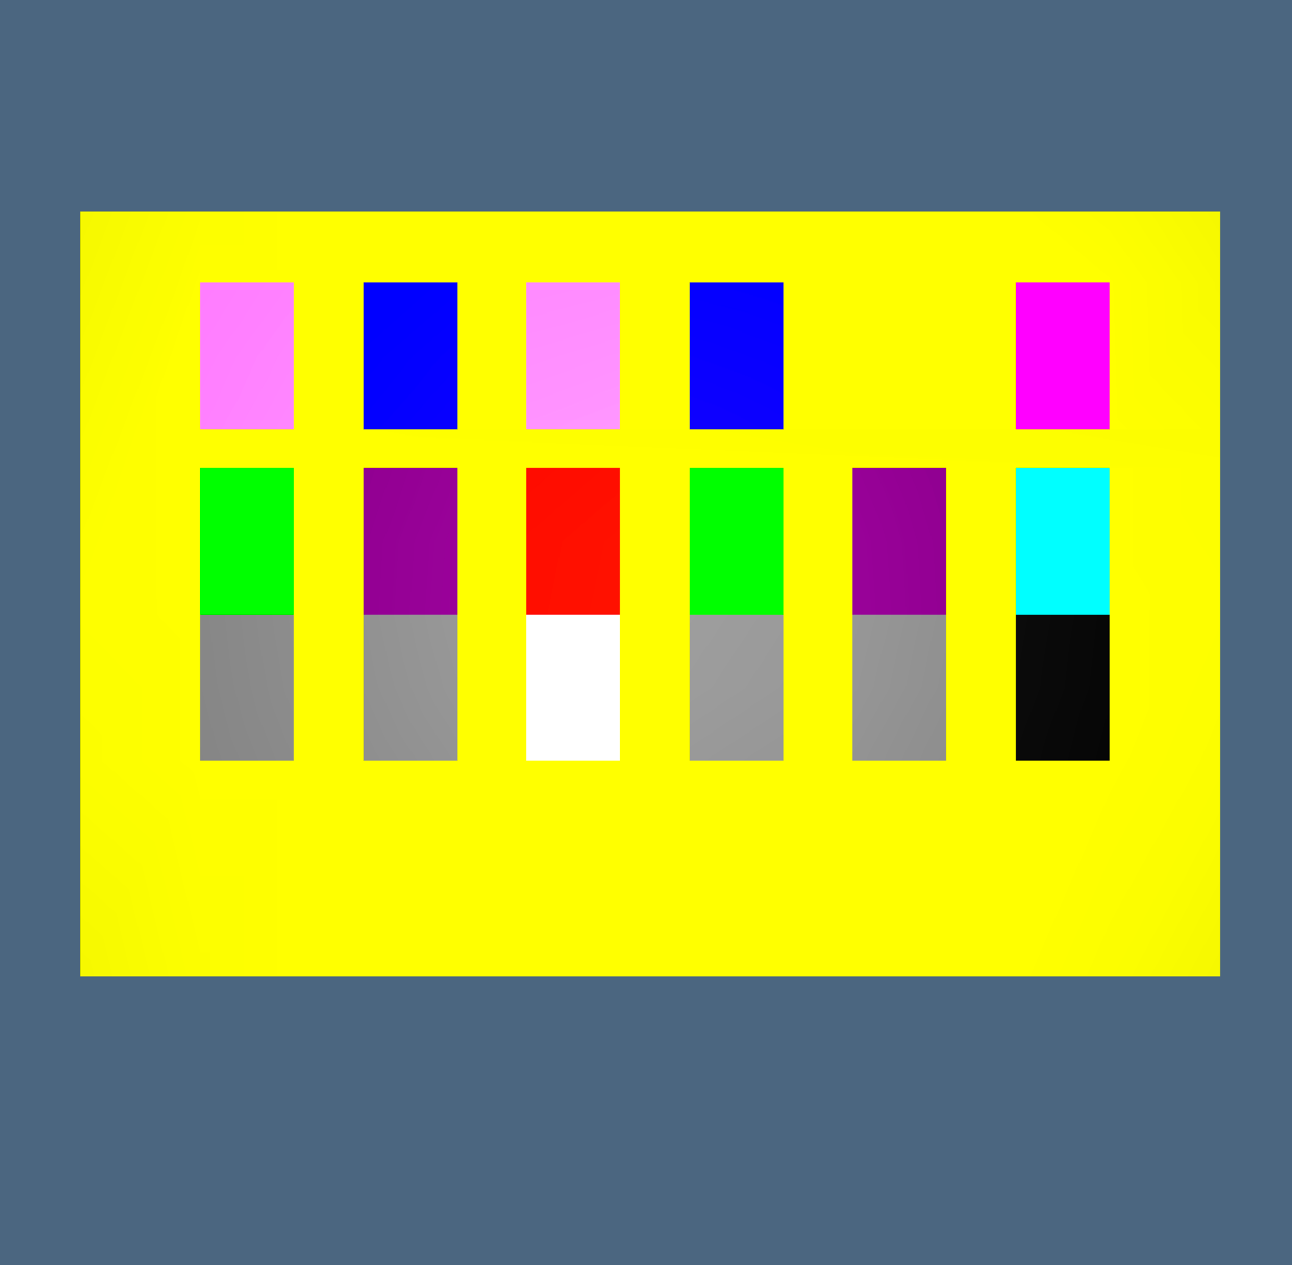
\includegraphics[height=0.325\linewidth,width=0.325\linewidth]{images/facade-b} 
   
\includegraphics[height=0.325\linewidth,width=0.325\linewidth]{images/facade-c} 

   \caption{From top to bottom, left to right: 
   (a) numbering of elementary cycles of a 2-complex with a hole in a 2-cell; (b) color display of 2-cells; (c) boundary of the 2-chain $\{f_0, f_1, f_2\}$, codified in coordinates as \texttt{[1,1,1,0]}. 
   (d) cycles of a 2-complex with nested 2-cells and non-manifold points; (e) color display of 2-cells; (f) boundary of the 2-chain $\{f_0,f_1,f_2,f_3\}$. 
   (g) The 2-complex modeling a building front; (h) color display of 2-cells; (i) solid display of elementary 2-chain $\{f_4\}\subset\texttt{FV}$, of high topological genus, codified in coordinates by the array \texttt{[$0,0,0,0,1,0,\ldots,0$]} of length \texttt{len(FV)}.}
   \label{fig:example}
\end{figure}



\subsection{Construction of LAR of 2-faces}

The contruction of faces in \texttt{FV} begins by computing the containment relation between all pairs of elementary cycles in $\mathcal{C}$.

Since they are boundary 1-chains of 2-chains corresponding to either maximal biconnected components of (\texttt{V}, \texttt{EV}) graph, the cycles in $\mathcal{C}$ cannot have intersection, except possibly on common vertices, corresponding to \emph{separation nodes} of the graph.
In order to test if $c_h$ is either \emph{internal} or \emph{external} to $c_k$, for $c_h, c_k \in \mathcal{C}$, it is sufficient to test the containment in $c_k$ of a single point \emph{internal} to $c_h$. 

We construct the binary matrix of the containment relation, which is anti-symmetric, reflexive and transitive.
Therefore the containment relation is a partial order, that can be represented as the DAG (Directed Acyclic Graph) of its transitive reduction,  often called \emph{Hasse diagram}.

The Hasse diagram of this relation is either a single tree or a forest, i.e.~a set of trees without common nodes, depending on the connection of the domain.
By numerating the nodes with their level number, defined as the integer distance of the node from the tree roots, and by deleting the arcs with starting node odd, we get a forest of trees with two levels, whose root(s) correspond to the exterior cycle(s) and whose leaves correspond to the internal holes of the faces.

Every such small tree (``sapling") of cycles, possibly reduced to the only root, in case of a face without holes, 
will correspond to a 2-cell of the 2-complex.


\subsection{Solid display of a 2-complex}

Let we start with a triple LAR model \texttt{(V,FV,EV)}.

First we compute the signed boundary operator. Then for each cycle $c$ in $\mathcal{C}$ we have a list of signed boundary edges. The loops of each cycle are extracted and classified as external or internal loops, and returned  as circularly ordered sequences of vertex indices.  Then the kind as manifold or non-manifold of $c$ is computed, by comparing the number of edges with the number of vertices. 

The non-manifold vertices are possibly signed, and the transformation from a list of vertex indices to a list of vertices (i.e.~list of lists of real coordinates) is applied.

Finally, every non-manifold vertex is moved in general position by applying to it a small translation perturbation towards the \emph{interior} of the cycle. The translation vector is computed by vector summation of the two adjacent tangent vectors incident to the vertex. Each incident vector is computed by properly orienting the vector difference between two consecutive vertices. 

For each set of disentangled loops, given as arrays of points without repetition, the appropriate functions of the python package \emph{Poly2tri}, named \texttt{p2t}, are called, returning a list of triples of 2D points corresponding to the generated triangulation of the face, possibly holding holes corresponding to the interior loops, if any.





\section{Implementation}
%===============================================================================


\subsection{Winged-inspired algoritm for computation of all elementary cycles}

In this section we introduce a novel implementation of the algorithm for computing all the cycles  from a two-dimensional LAR model. It is mostly based on the very simple idea that each edge (i.e.~every element of the \texttt{EV} list) must be used twice, in the opposite orientations. Therefore, a list \texttt{edgeCounts}, indexed by edge indices, stores dinamically the number of times that each edge was already used, of course starting from zero. 
    
\paragraph{Extract all cycles from a LAR pair model}

The \texttt{makeCycles} function takes as input a LAR pair model \texttt{(V,EV)}, and returns as output the list of 1-chains \texttt{cycles}, implemented as lists of vertex indices. The function starts with initializing the used variables, using as first \texttt{edge} of the first cycle the 0 edge, and as first \texttt{vertex} its corresponding first vertex. The existence of edges that have not completed their usage is codified by the truth value of the \texttt{unusedEdges} predicate. Just notice that the list \texttt{VE} of edges inciding on vertices and indexed by vertices is the one returned by the \texttt{edgeSlopeOrdering} function, that provides a sorting on angles formed with the horizontal line (i.e.~on absolute slope) of the incident edges. 

%%-------------------------------------------------------------------------------
%D Extract all cycles from a LAR pair model
%{""" Extract all cycles from a LAR pair model """ 
%import inters
%def makeCycles(model):
%    theModel = copy.copy(model)
%    V,EV = theModel
%    VE = inters.edgeSlopeOrdering(theModel)
%    unusedEdges = True
%    cycles,ecycles = [],[]
%    edgeCounts = [0 for edge in EV]
%    edge,vertex = 0,EV[0][0]
%    edgeCounts[0] = 1
%    print "edgeCounts =",edgeCounts
%    while unusedEdges:
%        theCycles = extractCycle(edgeCounts,EV,VE,edge,vertex,[vertex],[edge])
%        print "edgeCounts =",edgeCounts
%        cycles += [theCycles[0]]
%        ecycles += [theCycles[1]]
%        unusedEdges,edge,vertex = takeEdgeVertex(edgeCounts,EV)
%        edgeCounts[edge] += 1
%    return cycles,ecycles
%}
%%-------------------------------------------------------------------------------

\paragraph{Extract all cycles from a LAR pair model}
%-------------------------------------------------------------------------------
@D Extract all cycles from a LAR pair model
@{""" Extract all cycles from a LAR pair model"""

@< Incidence vertices-edges, sorted by angle @>
@< Computation of first and next edges of a cycle @>
@< Search for both vertex and edge cycles @>

def makeCycles(model):
    V,EV = model
    cycles_data = find_cycles (V, EV)
    vcycles,ecycles = cycles_data['v_cycles'],cycles_data['e_cycles']
    return [vcycle[:-1] for vcycle in vcycles],ecycles
@}
%-------------------------------------------------------------------------------


\paragraph{Incidence vertices-edges, sorted by angle}
%-------------------------------------------------------------------------------
@D Incidence vertices-edges, sorted by angle
@{""" Incidence vertices-edges, sorted by angle"""
def compute_angle (P, V):
    def sub (v1, v2):
        return [v1[0] - v2[0], v1[1] - v2[1]]
    point = sub(V, P)
    angle = math.atan2(point[1], point[0])
    return angle

def compute_incidences (V, EV):
    incidences = []
    for i in range(len(V)):
        vertex = V[i]
        incidence = []
        for j in range(len(EV)):
            edge = EV[j]
            endpoint = None
            if (edge[0] == i):
                endpoint = edge[1]
                position = 1
            if (edge[1] == i):
                endpoint = edge[0]
                position = 0
            if (endpoint != None):
                    incidence.append({
                        'index': j,
                        'endpoint': endpoint,
                        'angle': compute_angle(vertex, V[endpoint]),
                        'edge': edge,
                        'position': position
                    })
        incidence = sorted(incidence, key=lambda item: item['angle'], reverse=True)
        incidences.append(incidence)
    # print map(lambda l: map(lambda i: i['angle'], l), incidences)
    return incidences
@}
%-------------------------------------------------------------------------------

\paragraph{Computation of first and next edges of a cycle}
%-------------------------------------------------------------------------------
@D Computation of first and next edges of a cycle
@{""" Computation of first and next edges of a cycle"""
def get_starting_edge (incidences, ev_mapping):
    for e in range(len(ev_mapping)):
        if (ev_mapping[e]['color'] < 2):
            direction = 0 if ev_mapping[e]['direction'] == 1 else 1
            color(ev_mapping, e, direction)
            return {
                'edge': e,
                'position': direction }
    return None

def get_next_edge (EV,incidences, edge, position):
    items = incidences[EV[edge][position]]
    for j in range(len(items)):
        item = items[j]
        if (item['index'] == edge):
            out = items[mod(j + 1, len(items))]
            return {
                'edge': out['index'],
                'vertex': out['endpoint'],
                'position': out['position'] }
    return None

def color (ev_mapping, index, direction):
    ev_mapping[index]['color'] += 1
    ev_mapping[index]['direction'] = 1 if direction == 1 else -1
@}
%-------------------------------------------------------------------------------


\paragraph{Search for both vertex and edge cycles}
%-------------------------------------------------------------------------------
@D Search for both vertex and edge cycles
@{""" Search for both vertex and edge cycles"""
def compute_ev_mapping (EV):
    ev_mapping = []
    for i in range(len(EV)):
        ev_mapping.append({ 'color': 0, 'direction': 0 })
    return ev_mapping

def find_cycles (V, EV):
    ev_mapping = compute_ev_mapping(EV)
    incidences = compute_incidences(V, EV)
    V_cycles = []
    E_cycles = []
    counter = 1
    start = get_starting_edge(incidences, ev_mapping)
    while (start != None):
        V_cycle = [ EV[start['edge']][mod(start['position'] + 1, 2)], 
                    EV[start['edge']][start['position']] ]
        E_cycle = [start['edge']]
        next = get_next_edge(EV,incidences, start['edge'], start['position'])
        while (next['edge'] != start['edge']):
            V_cycle.append(next['vertex'])
            E_cycle.append(next['edge'])
            color(ev_mapping, next['edge'], next['position'])
            next = get_next_edge(EV,incidences, next['edge'], next['position'])
        E_cycles.append(E_cycle)
        V_cycles.append(V_cycle)
        """
        print '############## CYCLE ', counter
        print 'EDGES:', E_cycle
        print 'VERTICES:', V_cycle
        print 'START', 'edge:', start['edge'], 'position:', start['position']
        print 'COUNTER:', map(lambda e: e['color'], ev_mapping)
        print '\n'
        """
        start = get_starting_edge(incidences, ev_mapping)
        counter += 1
    return {
        'v_cycles': V_cycles,
        'e_cycles': E_cycles,
        'ev_mapping': ev_mapping }
        
@< Testing the extraction of cycles of a LAR 2-complex @>
@}
%-------------------------------------------------------------------------------


\paragraph{Testing the extraction of cycles of a LAR 2-complex}
%-------------------------------------------------------------------------------
@D Testing the extraction of cycles of a LAR 2-complex
@{""" Testing the extraction of cycles of a LAR 2-complex"""
if __name__=="__main__":

    V = [[0.5774, 1.0], [1.0, 1.0], [1.1547, 0.0], [1.0, 0.0], [0.0, 0.0], [0.0, 0.732], [1.0, 0.1547], [0.732, 0.0], [1.0491, 0.183], [-0.317, 0.549], [1.0, 0.268], [0.183, -0.3169], [0.5491, 1.049], [0.4642, 1.0], [0.0, -0.4226], [0.0, 1.0]]
                                                                                                                                                                                 
    EV = [[0, 1], [2, 3], [5, 4], [7, 6], [2, 8], [3, 6], [4, 9], [0, 10], [9, 5], [8, 10], [7, 11], [12, 13], [6, 8], [6, 10], [4, 7], [4, 11], [4, 14], [5, 15], [11, 14], [0, 12], [13, 15], [0, 13], [1, 10], [3, 7], [5, 13]]
    
    cycles_data = find_cycles(V, EV)
    """
    print '############## OUTPUT'
    print 'EDGES:'
    print cycles_data['e_cycles']
    print '\n'
    print 'VERTICES:'
    print cycles_data['v_cycles']
    """
    VIEW(EXPLODE(1.2,1.2,1)(AA(POLYLINE)([[V[v] for v in vcycle] for vcycle in cycles_data['v_cycles'][1:]])))
@}
%-------------------------------------------------------------------------------


\paragraph{Return a feasible pair edge/vertex}
The function \texttt{takeEdgeVertex} is used to return a new triple of values for the variables \texttt{unusedEdges,edge,vertex} used by is calling function \texttt{makeCycles}.

%-------------------------------------------------------------------------------
@D Return a feasible pair edge/vertex
@{""" Return a feasible pair edge/vertex """ 
def takeEdgeVertex(edgeCounts,EV):
    e = edgeCounts.index(min(edgeCounts))
    if edgeCounts[e] < 2: 
        v = EV[e][0]
        return True,e,v
    else: return False,0,0
@}
%-------------------------------------------------------------------------------


\paragraph{Extract a single edge/vertex cycle}
The \texttt{extractCycle} recursive function given below is used to return a new cycle extracted from the \texttt{EV} list, and starting with the pair \texttt{e,v}. While the abstract formulation of a cycle is a closed 1-chain, its actual implementation here is as an ordered sequence (list) of 0-cells (vertices). Notice that every time an edge \texttt{e} is used in a cycle, its orientation is reversed by exchanging the storage positions of its first and second vertex.  The base case of the recursion checks if the \texttt{nextVertex} to be included in the list is different from the first element of the \texttt{cycle}. If equal, the recursion is stopped and the constructed cycle returned.
 
%-------------------------------------------------------------------------------
@D Extract a single edge/vertex cycle
@{""" Extract a single edge/vertex cycle """ 
def succ(e,seq):
    return seq[(seq.index(e)+1) % len(seq)]
   
def extractCycle(edgeCounts,EV,VE,e,v,cycle,ecycle):        
    nextEdge = succ(e,VE[v])
    nextVertex, = set(EV[nextEdge]).difference({v})
    if nextVertex != cycle[0]:
        cycle.append(nextVertex)
        ecycle.append(nextEdge)
        edgeCounts[nextEdge] += 1 
        v1,v2 = EV[e]
        extractCycle(edgeCounts,EV,VE,nextEdge,nextVertex,cycle,ecycle)
        EV[e] = v2,v1
    return cycle,ecycle
@}
%-------------------------------------------------------------------------------
    


\subsection{Containments between non intersecting cycles}

In this section we compute the containment relation between non-intersecting cycles generated on 2-faces by the incident faces. This step is preparatory to the representation of fragmented 2-faces --- embedded in 2D --- as LAR data structures, to be subsequently restored in the ambient 3D and sticked together to generate the the 2-skeleton of a Boolean complex.

For this purpose, the set of non-intersecting cycles, as lists of edges, are returned in the \texttt{EVs} array by the \texttt{biconnectedComponent} function. The pair \texttt{V,EVs} is therefore passed as input to the \texttt{computeCycleLattice} function, that returns a dense matrix with elements in $\{-1,0,1\}$, where the element $i,j$ either contains $0$ if anyone (and hence all) of vertices of cycle $j$-th is \emph{external} to cycle $i$-th, or contains $1$ if anyone (and hence all) of vertices of cycle $j$-th is \emph{internal} to cycle $i$-th, or finally contains $-1$ if anyone (and hence all) of vertices of cycle $j$-th is \emph{on boundary} of cycle $i$-th. The last condition may hold only for diagonal elements $i,j$ where $i=j$.

The returned \texttt{latticeArray} matrix of dimension $n\times n$, where $n$ is the number of non-intersecting cycles on a fragmented 2D face, is the used by the \texttt{cellsFromCycles} function, that return a list of lists of cycles, each one defining the boundary of a single connected but possibly non path-connected 2-cell in the LAR representation of the fragmented 2-complex. 

\paragraph{Classification of non intersecting cycles}

The function \texttt{computeCycleLattice} takes as input the pair \texttt{V,EVs}, where $V$ is the list of vertices and \texttt{EVs} is the list of cycles of a fragmented 2-cell in 2D. Each \texttt{EVs} element is given as a list of edges, given os pairs of integer vertex indices.
The returned \texttt{latticeArray} matrix --- characterizing the incidences between cycles --- has dimension $n\times n$.

\paragraph{Remark on interior point vs cycle's vertex classification }

When reconstructing the containment lattice of component cycles of a boundary chain, the strategy of testing for containment a single vertex of a cycle against another cycle does not work, since the tested vertex might stay in non-manifold position, so that---while internal points stay either internal or external to the target cycle, the result of the containment test would be of type \texttt{.on.}, corresponding to test point on the boundary of the target cycle, so producing a wrong containment lattice.

So, in computing the $(k,h)$ term of the containment matrix, stored witin the \texttt{latticeArray} below, we cannot in general use the simpler testing \texttt{point = V[i]}, but another \texttt{point} guaranteed to belong to a close neighborhood of it, in the interior of \texttt{EVs[h]}.

For this reason the \texttt{internalTo} function is introduced, that returns a \texttt{point} that is internal to the \texttt{ev} cycle, and in particular internal to the plane sector interior to the angle formed by the first vertex, named \texttt{v}, of \texttt{ve} (edges incident on vertices) array, that is incident only to two edges (and hence is not in non-manifold position). The function will work with both acute and ottuse interior angles incident on \texttt{v}.

%-------------------------------------------------------------------------------
@D Classification of non intersecting cycles
@{""" Classification of non intersecting cycles """
def internalTo(V,ev):
    classify = pointInPolygonClassification((V,ev))
    ve = invertRelation(ev)
    for v,edgeIndices in enumerate(ve):
        if len(edgeIndices) == 2: break
    v1,v2 = set(CAT([list(ev[e]) for e in edgeIndices])).symmetric_difference([v])
    vect1 = VECTDIFF([V[v1],V[v]])
    vect2 = VECTDIFF([V[v2],V[v]])
    point = VECTSUM([ V[v], SCALARVECTPROD([ 0.05, VECTSUM([vect1,vect2]) ])])
    if classify(point) == "p_out":
        point = VECTSUM([ V[v], SCALARVECTPROD([ -0.05, VECTSUM([vect1,vect2]) ])])
    return point
    
def computeCycleLattice(V,EVs):
    n = len(EVs)
    latticeArray = []
    interiorPoints = [internalTo(V,ev) for k,ev in enumerate(EVs)]
    for k,ev in enumerate(EVs):
        row = []
        classify = pointInPolygonClassification((V,ev))
        for h in range(n):
            i = EVs[h][0][0]
            #point = V[i]
            point = interiorPoints[h]
            test = classify(point)
            if h==k: row += [-1]
            elif test=="p_in": row += [1]
            elif test=="p_out": row += [0]
            elif test=="p_on": row += [-1]
            else: print "error: in cycle classification"
        latticeArray += [row]
    for k in range(n):
        for h in range(k+1,n): 
            if latticeArray[k][h] == latticeArray[h][k]:
                latticeArray[k][h] = 0
    return latticeArray
@}
%-------------------------------------------------------------------------------

\paragraph{Extraction of path-connected boundaries}

The function \texttt{cellsFromCycles}, given by the script below, takes as input the cycle-incidence matrix \texttt{latticeArray}, and return the list \texttt{out} of lists of cycles, providing the boundaries of a decomposition into connected (but possibly non path-connected) 2-cells of the fragmented 2-face whose non-intersecting cycles were computed as output of the \texttt{biconnectedComponent} function. 

First the \texttt{sons} of each cycle are computed, i.e. the indices of cycles containd in it, as well as the \texttt{level} of every cycle, i.e.~their position within the lattice of the containment relation (that is a partial order). 
The level of a cycle is computed as the sum of elements in its matrix column. The roots of the lattice, i.e.~the more external cycles have level -1; the following levels have values $0,1,2,...$, respectively.

Then the cycles are ordered in the encreasing value of their level (or \emph{rank}), and finally the significant subsets of disjoint cycles are extracted within the \texttt{out} list, starticg from the root cycle(s). The important properties exploited for the extraction are the following: (a) the first element of each sublist is the external boundary cycle, whereas the following cycles, if any, are its internal boundaries; (b) the rank difference between each external and internal boundary must be less or equal to one. It will be 0 only whe the sublist contains only one element (the external boundary) wich is being compared with itself.

Finally the sublists are pruned, by eliminating those whose first element has benn previously used within some of the previous ones (of course: was already used as an internal cycle).

%-------------------------------------------------------------------------------
@D Extraction of path-connected boundaries
@{""" Extraction of path-connected boundaries """
def cellsFromCycles (latticeArray):
    n = len(latticeArray)
    sons = [[h]+[k for k in range(n) if row[k]==1] for h,row in enumerate(latticeArray)]
    level = [sum(col) for col in TRANS(latticeArray)]
    
    def rank(sons): return [level[x] for x in sons]
    preCells = sorted(sons,key=rank)

    def levelDifference(son,father): return level[son]-level[father]
    root = preCells[0][0]
    out = [[son for son in preCells[0] if (levelDifference(son,root)<=1) ]]
    for k in range(1,n):
        father = preCells[k][0]
        inout = [son for son in preCells[k] if levelDifference(son,father)<=1 ]
        if not (inout[0] in CAT(out)):
            out += [inout]
    return out        
@}
%-------------------------------------------------------------------------------

\paragraph{Testing containments between non intersecting cycles}

The test code for verifying the approch to computation of the containment lattice between non intersecting cycles is given below. Three test files, named respectively \texttt{lattice}, \texttt{lattice1} and \texttt{lattice2},  with the different situations shown in Figure~\ref{fig:lattice}, may be imported from the directory \texttt{test/svg/inters/}. Other tests may be easily generated by inserting in this directory some \texttt{.svg} files generated with a drawing program. 

%-------------------------------------------------------------------------------
@O test/py/inters/test15.py
@{""" Testing containments between non intersecting cycles """
from larlib import *

filename = "test/svg/inters/facade.svg"
lines = svg2lines(filename)
VIEW(STRUCT(AA(POLYLINE)(lines)))

V,EV = lines2lar(lines)
V,EVs = biconnectedComponent((V,EV))
# candidate face
FVs = AA(COMP([list,set,CAT]))(EVs)

latticeArray = computeCycleLattice(V,EVs)

for k in range(len(latticeArray)):
    print k,latticeArray[k]

VV = AA(LIST)(range(len(V)))
submodel = STRUCT(MKPOLS((V,EV)))
VIEW(larModelNumbering(1,1,1)(V,[VV,EV,FVs],submodel,0.15)) 
@}
%-------------------------------------------------------------------------------


\begin{figure}[htbp] %  figure placement: here, top, bottom, or page
   \centering
   \fbox{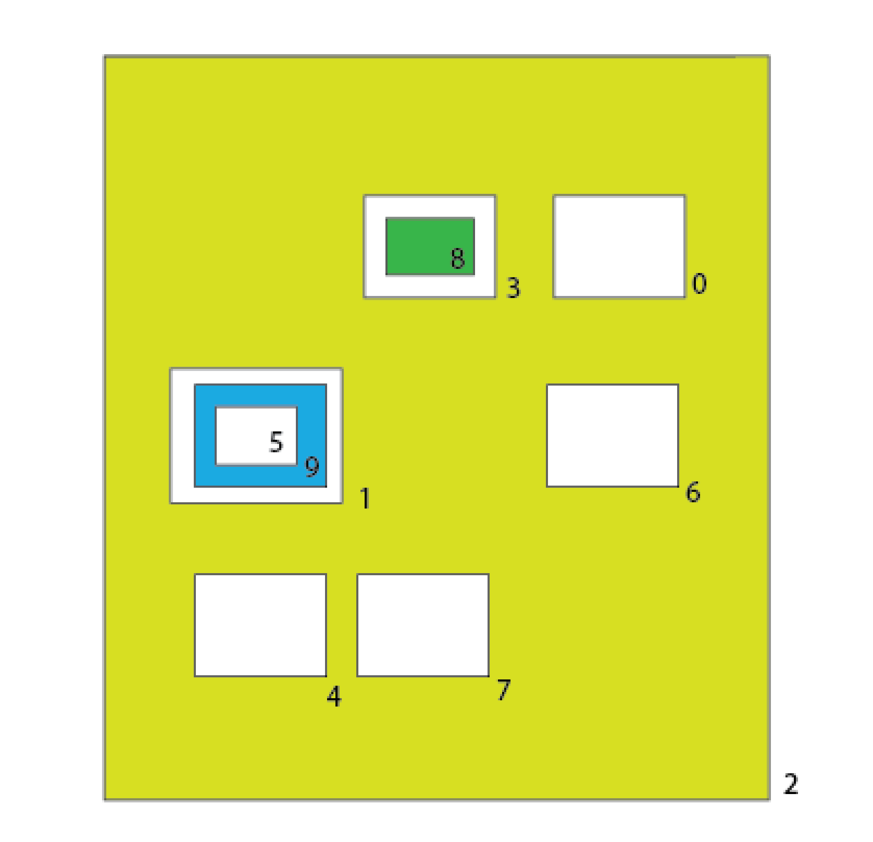
\includegraphics[height=0.24\linewidth,width=0.24\linewidth]{images/lattice0}}
   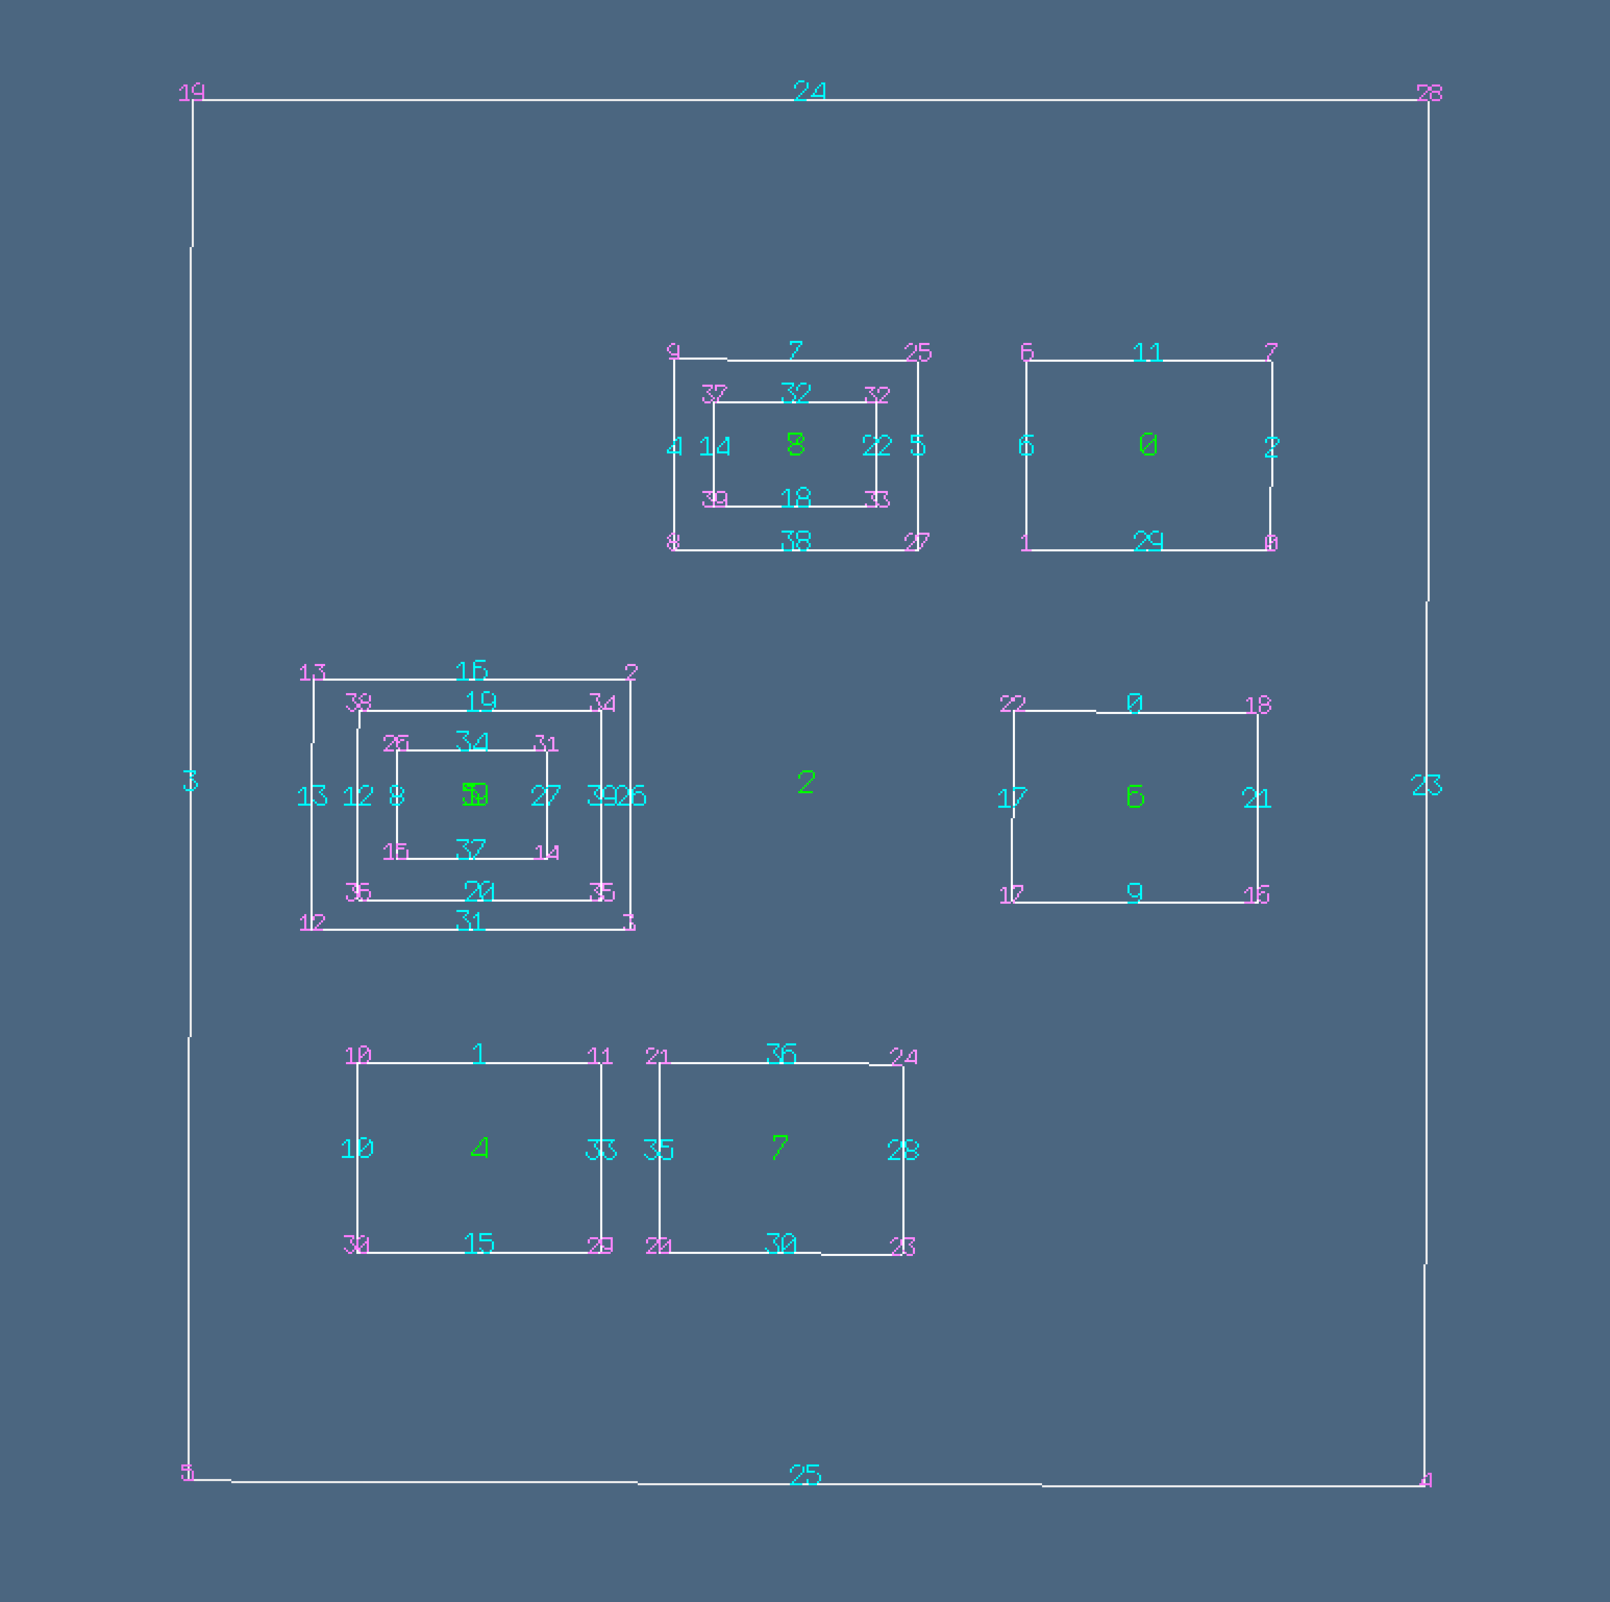
\includegraphics[height=0.24\linewidth,width=0.24\linewidth]{images/lattice1} 
   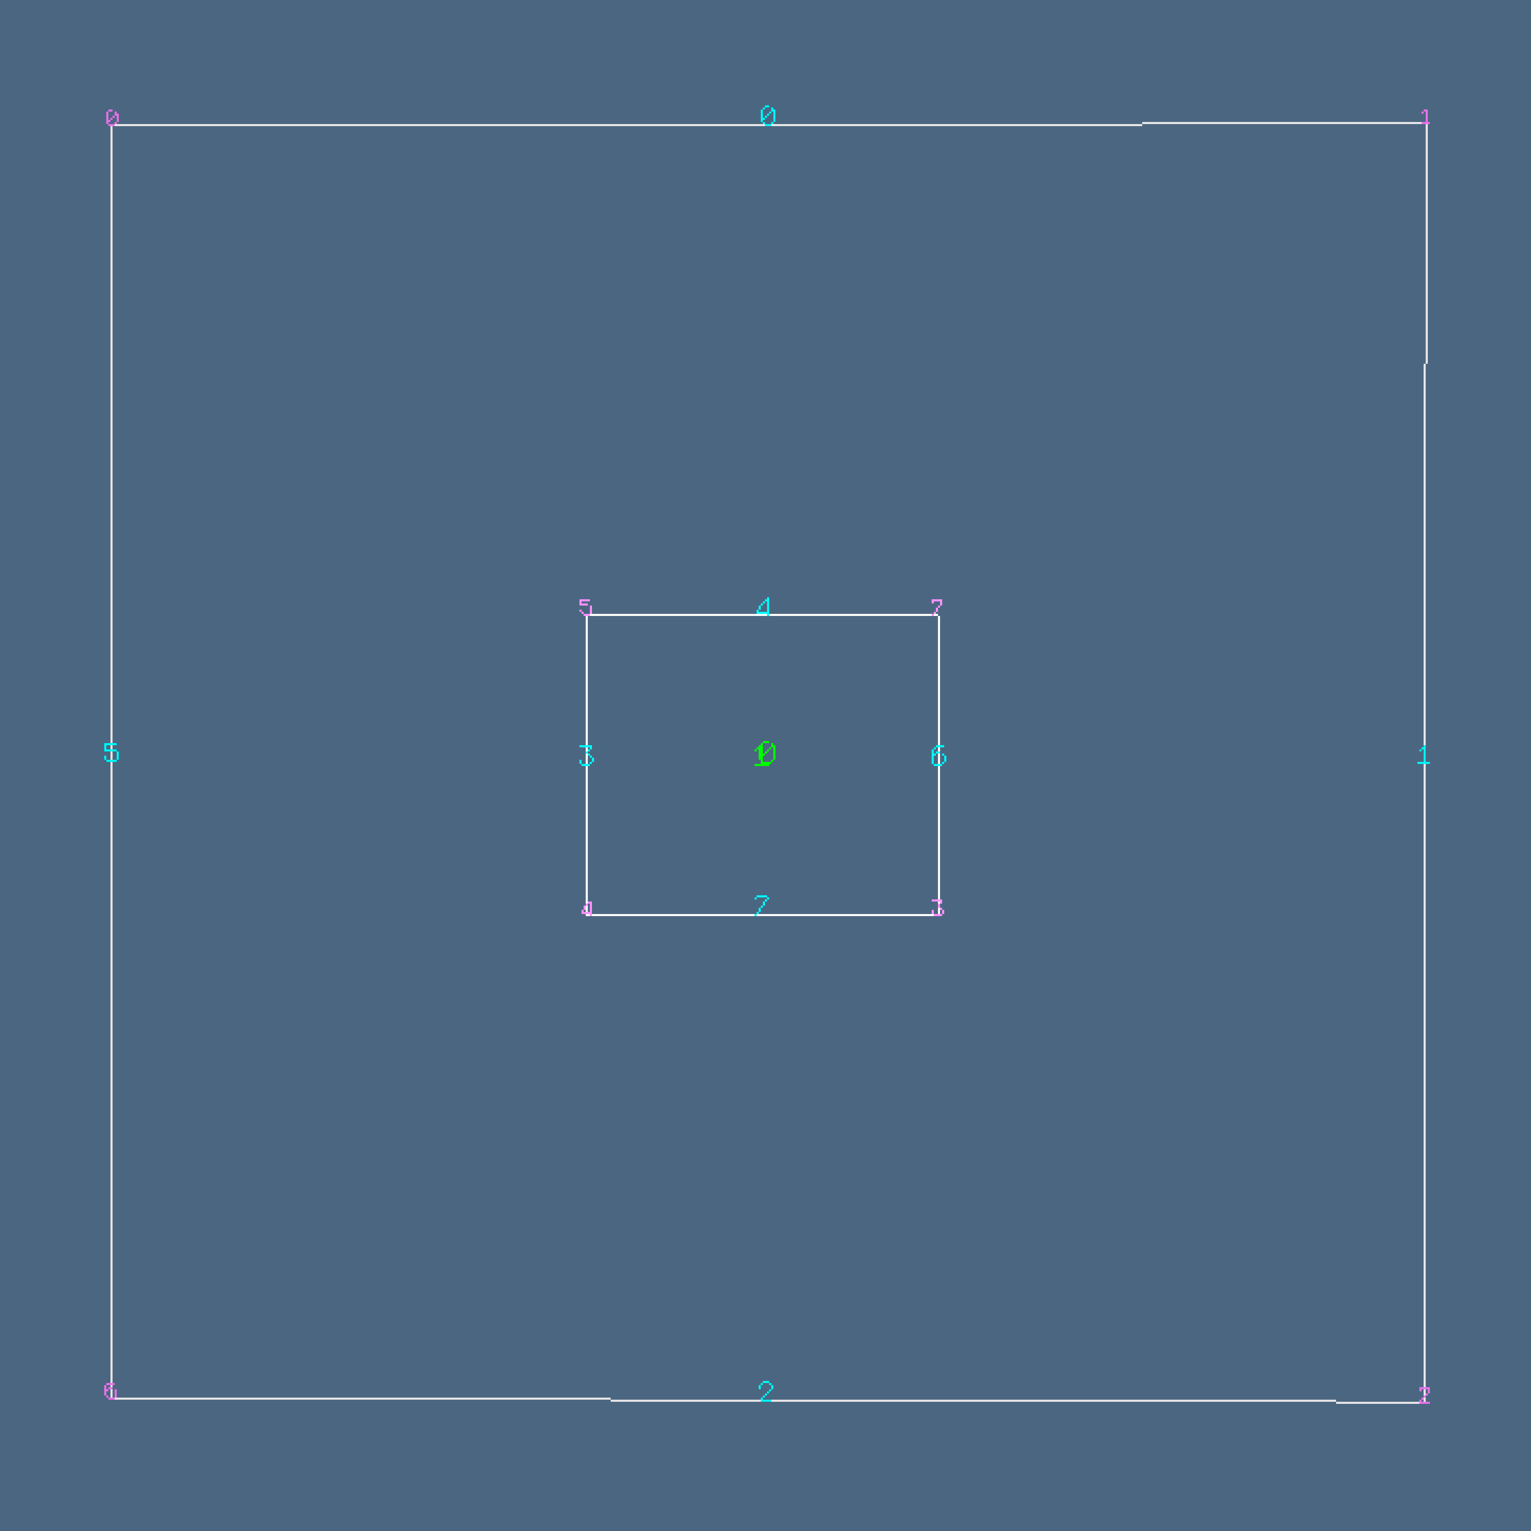
\includegraphics[height=0.24\linewidth,width=0.24\linewidth]{images/lattice2} 
   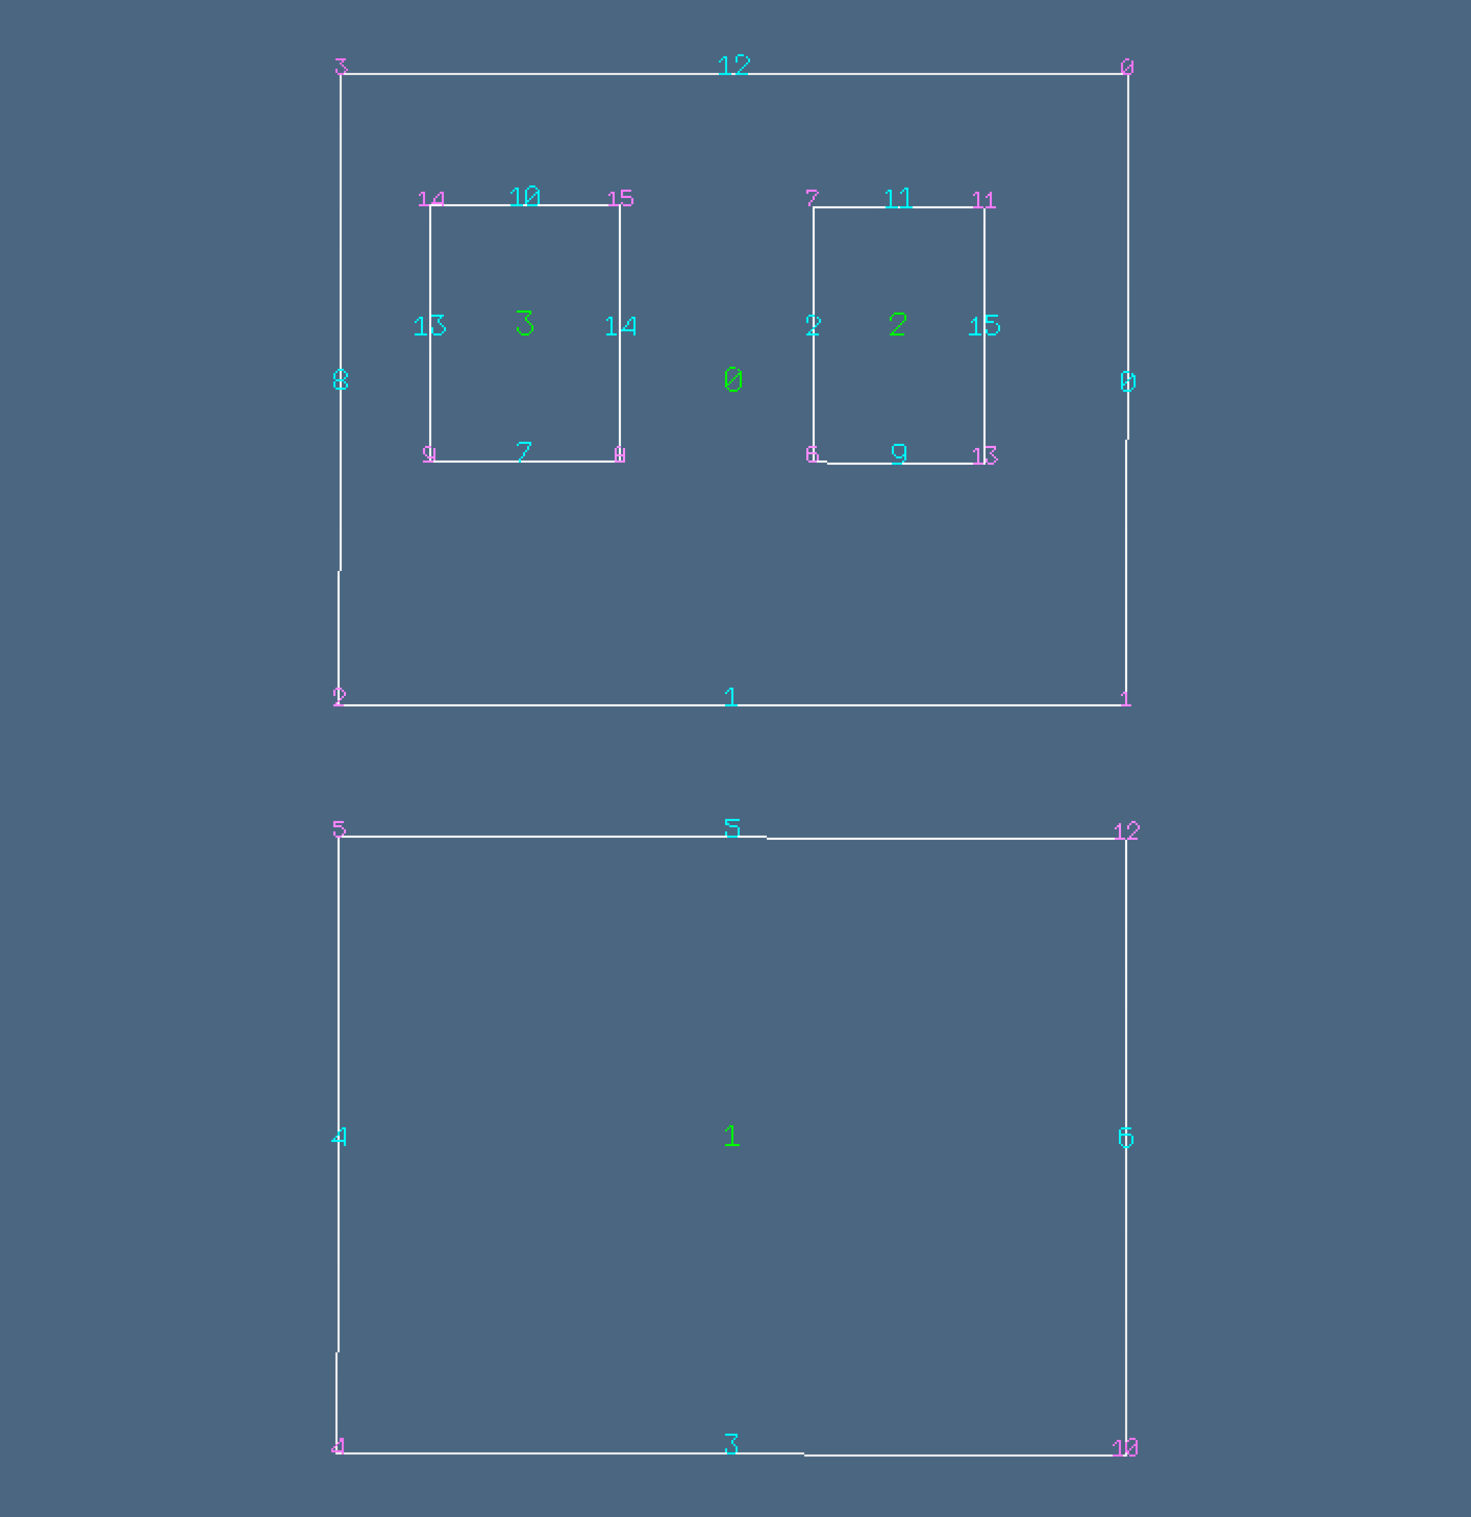
\includegraphics[height=0.24\linewidth,width=0.24\linewidth]{images/lattice3} 
   \caption{Some examples of nested non intersecting cycles. The corresponding solutions are given in the text.}
   \label{fig:example}
\end{figure}


\subsection{Reduction of multiple cycles to a single polyline}
\label{sec:singlepolyline}
%~~~~~~~~~~~~~~~~~~~~~~~~~~~~~~~~~~~~~~~~~~~~~~~~~~~~~~~~~~~~~~~~~~~~~~~~~~~~~~~

The reduction of a lattice of non-intersecting 1-cycles on the boundary of a 2-cell into a single polyline is performed using a scan-line algorithm.

In order to filter the complications induced by edges aligned with the reference axes, first we perform a transformation of vertices from Cartesian to polar coordinates (see Figure~\ref{fig:polarholes}).

Then a specialized scan-line algorithm is executed, producing a set of \emph{bridge-edges}~\cite{Yamaguchi:85} that, added in double instance to the set \texttt{EV} of the LAR of the 2-cell, allow for a triangulation of its interior using the algorithm provided by the \texttt{poly2tria} module.

\begin{figure}[htbp] %  figure placement: here, top, bottom, or page
   \centering
   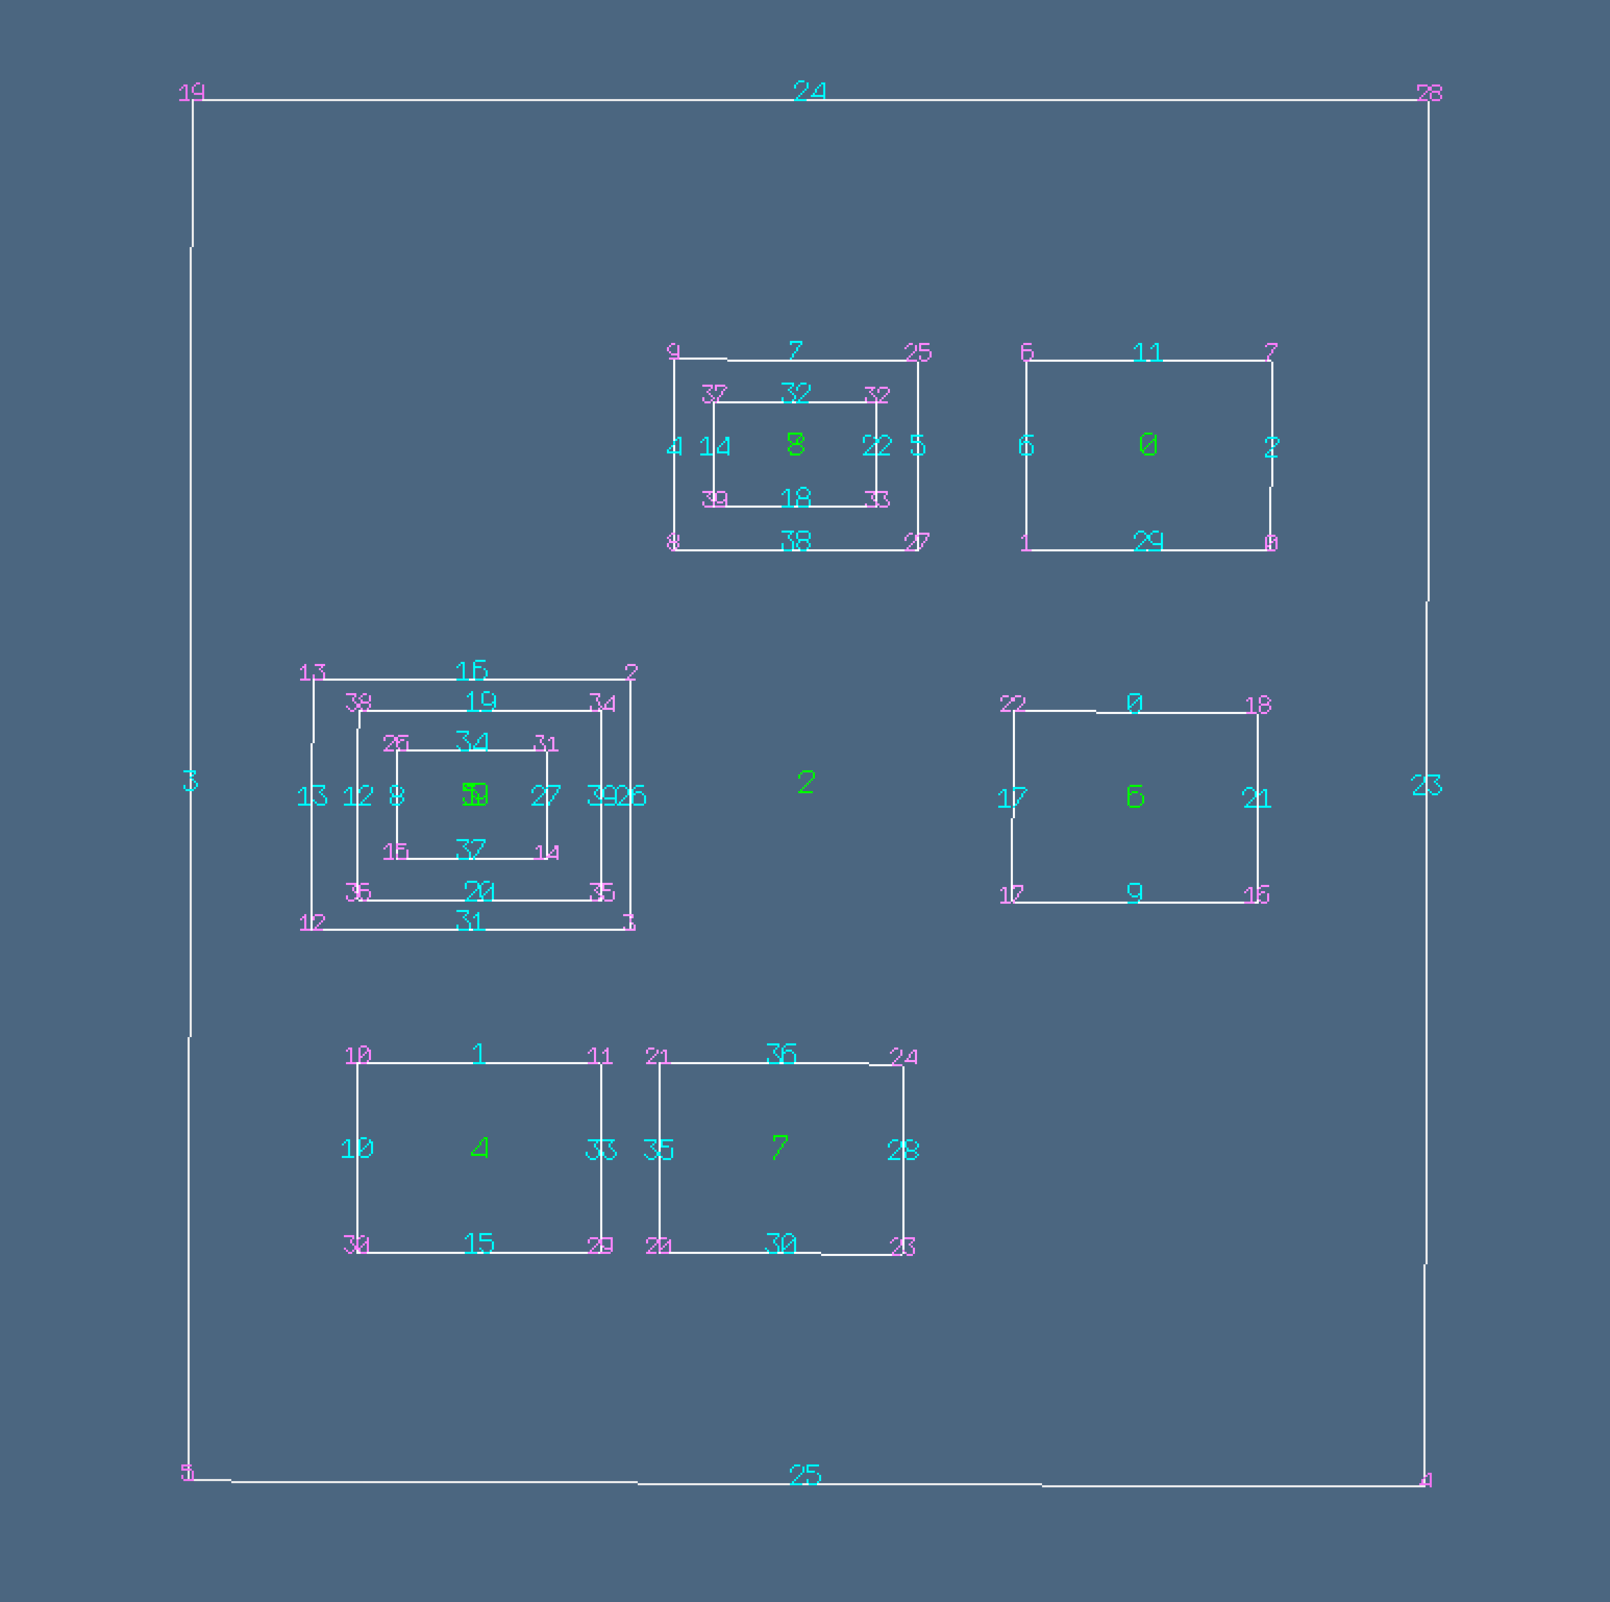
\includegraphics[height=0.33\linewidth,width=0.33\linewidth]{images/lattice1} 
   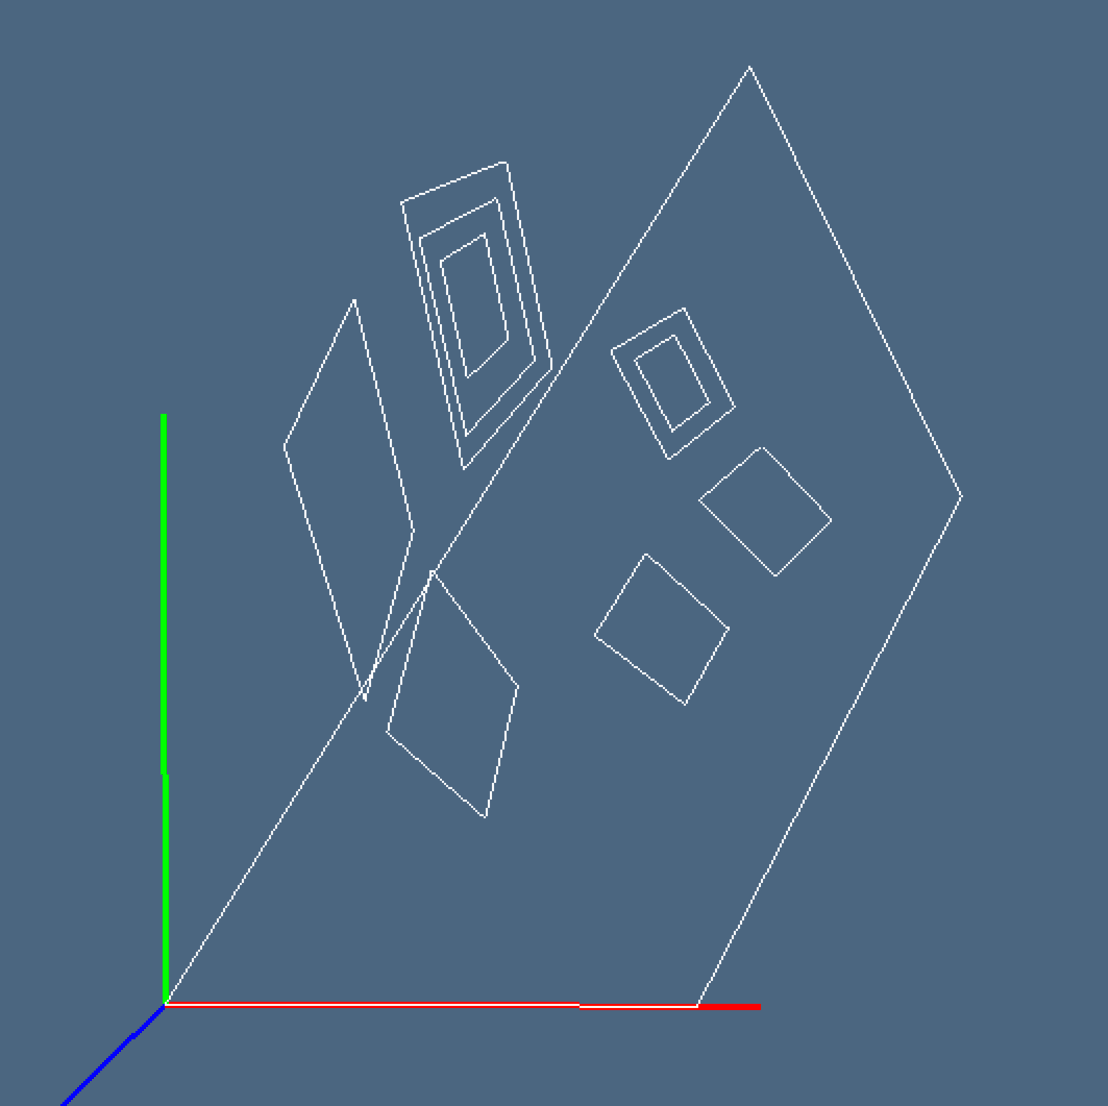
\includegraphics[height=0.33\linewidth,width=0.33\linewidth]{images/polarholes} 
   \caption{A set of non-intersecting boundary cycles in Cartesian and polar coordinates, using (improperly) an Euclidean metric in the transformed space.}
   \label{fig:polarholes}
\end{figure}


\paragraph{Transforming to polar coordinates}

The transformation from Cartesian to polar coordinates of the vertices of a two-dimensional LAR model is given in the following script. An image of such transformation is shown in Figure~\ref{fig:polarholes}. It is only used here to put the vertex coordinates in general position, so simplifying the scan-line algorithm.
%-------------------------------------------------------------------------------
@D Transforming to polar coordinates 
@{""" Transforming to polar coordinates """
def cartesian2polar(V):    
    Z = [[sqrt(x*x + y*y),math.atan2(y,x)] for x,y in V]
    VIEW(STRUCT(MKPOLS((Z,EV))))
    return Z
@}
%-------------------------------------------------------------------------------


\paragraph{Scan line algorithm}
%-------------------------------------------------------------------------------
@D Scan line algorithm 
@{""" Scan line algorithm """
def scan(V,FVs, group,cycleGroup,cycleVerts):
    bridgeEdges = []
    scannedCycles = []
    for k,(point,cycle,v) in enumerate(cycleGroup[:-2]):
        
        nextCycle = cycleGroup[k+1][1]
        n = len(FVs[group][cycle])
        if nextCycle != cycle: 
            if not ((nextCycle in scannedCycles) and (cycle in scannedCycles)):
                scannedCycles += [nextCycle]
                m = len(FVs[group][nextCycle])
                v1,v2 = v,cycleGroup[k+1][2]
                minDist = VECTNORM(VECTDIFF([V[v1],V[v2]]))
                for i in FVs[group][cycle]:
                    for j in FVs[group][nextCycle]:
                        dist = VECTNORM(VECTDIFF([V[i],V[j]]))
                        if  dist < minDist: 
                            minDist = dist
                            v1,v2 = i,j
                bridgeEdges += [(v1,v2)]
    return bridgeEdges[:-1]
@}
%-------------------------------------------------------------------------------

\paragraph{Scan line algorithm input/output}

The two-dimensional LAR \texttt{model} $\equiv$ \texttt{V,EV} was previously created by a \texttt{lines2lar(lines)} expression.

%-------------------------------------------------------------------------------
@D Scan line algorithm input/output
@{""" Scan line algorithm input/output """
def connectTheDots(model):
    V,EV = model
    V,EVs = inters.biconnectedComponent((V,EV))
    FV = AA(COMP([sorted,set,CAT]))(EVs)
    latticeArray = computeCycleLattice(V,EVs)
    cells = cellsFromCycles(latticeArray)
    FVs = [[FV[cycle] for cycle in cell] for cell in cells]
    
    indexedCycles = [zip(FVs[h],range(len(FVs[h])))   for h,cell in enumerate(cells)]
    indexedVerts = [CAT(AA(DISTR)(cell)) for cell in indexedCycles]
    sortedVerts = [sorted([(V[v],c,v) for v,c in cell]) for cell in indexedVerts]
    
    bridgeEdges = []
    cellIndices = range(len(cells))
    for (group,cycleGroup,cycleVerts) in zip(cellIndices,sortedVerts,indexedVerts):
        bridgeEdges += [scan(V,FVs, group,cycleGroup,cycleVerts)]
    return cells,bridgeEdges
@}
%-------------------------------------------------------------------------------

\paragraph{Orientation of component cycles of unconnected boundaries}

This step of the algorithm needs some preliminary computation, starting from the list \texttt{EV} of edges by vertices. Just notice that, at this point of the implementation (as the edges of a set of non intersecting cycles) they all are boundary edges, and hence the \texttt{edgeBoundary} variable can be filled with consecutive integers. The \texttt{edgeCycles} returned by \texttt{boundaryCycles} are very well characterized, according to how discussed in the description of the \texttt{Edge cycles associated to a closed chain of edges} paragraph.
The corresponding \texttt{vertexCycles} are first oriented accordingly to \texttt{boundaryCycles}, then rotated (as equivalent permutations) in order to put their element of minimum index in first position (accordingly to the numeration of cycles used in the variable \texttt{FVs}). Then, the \texttt{CVs} will be set to contain the circularly ordered vertices of the various boundary cycles of each LAR 2-cell, in a manner analogous to FVs, where the vertices are not circularly ordered. Finally, the first (i.e.~the \emph{external}) cycle of each cell is counterclockwise oriented, whereas the other cycles (i.e.~the \emph{internal} ones), are oriented clockwise.

%-------------------------------------------------------------------------------
@D Orientation of component cycles of unconnected boundaries 
@{""" Orientation of component cycles of unconnected boundaries """
def rotatePermutation(inputPermutation,transpositionNumber):
    n = transpositionNumber
    perm = inputPermutation
    permutation = range(n,len(perm))+range(n) 
    return [perm[k] for k in permutation]

def canonicalRotation(permutation):
    n = permutation.index(min(permutation))
    return rotatePermutation(permutation,n)

def setCounterClockwise(h,k,cycle,areas,CVs):
    if areas[cycle] < 0.0: 
        chain = copy.copy(CVs[h][k])
        CVs[h][k] = canonicalRotation(REVERSE(chain))

def setClockwise(h,k,cycle,areas,CVs):
    if areas[cycle] > 0.0: 
        chain = copy.copy(CVs[h][k])
        CVs[h][k] = canonicalRotation(REVERSE(chain))

def orientBoundaryCycles(model,cells):
    V,EV = model
    edgeBoundary = range(len(EV))
    edgeCycles,_ = boundaryCycles(edgeBoundary,EV)
    vertexCycles = [[ EV[e][1] if e>0 else EV[-e][0] for e in cycle ] for cycle in edgeCycles]
    rotations = [cycle.index(min(cycle)) for cycle in vertexCycles]
    theCycles = sorted([rotatePermutation(perm,n) for perm,n in zip(vertexCycles,rotations)])
    CVs = [[theCycles[cycle] for cycle in cell] for cell in cells]
    areas = signedSurfIntegration((V,theCycles,EV),signed=True)
    
    for h,cell in enumerate(cells):
        for k,cycle in enumerate(cell):
            if k == 0: setCounterClockwise(h,k,cycle,areas,CVs)
            else: setClockwise(h,k,cycle,areas,CVs)
    return CVs
@}
%-------------------------------------------------------------------------------

\paragraph{From nested boundary cycles to triangulation}
%-------------------------------------------------------------------------------
@D From nested boundary cycles to triangulation 
@{""" From nested boundary cycles to triangulation """    
def larTriangulation( (V,EV) ):
    V,FV,EV,polygons = inters.larFromLines([[V[u],V[v]] for u,v in EV])
    triangleSet = polygons2TriangleSet(V,polygons)
    return triangleSet
@}
%-------------------------------------------------------------------------------

\paragraph{Test example}
%-------------------------------------------------------------------------------
@O test/py/triangulation/test14.py 
@{""" Test example """    
from larlib import *
V,EV = ([[0.0, 0.0],
  [1.0, 0.0],
  [0.0, 1.0],
  [-0.536, 0.536],
  [-1.0, 1.0],
  [-0.036, 0.536],
  [-0.4227, 0.4227],
  [0.0773, 0.4227]],
 [[1, 0], (0, 6), (6, 7), [7, 5], [5, 3], (3, 6), [2, 1], [4, 3], [4, 2]])
 
model = V,EV

@}
%-------------------------------------------------------------------------------




\subsection{General composition of nested and non manifold cycles}
%-------------------------------------------------------------------------------
@D General composition of nested and non manifold cycles 
@{""" General composition of nested and non manifold cycles """

@< Trasform a non-manifold cycle of vertices into a manifold  @>
@< Check if some cycle is isolated (hence doubled) @>
@< From a non-contractible polygon to a list of triangles @>
@< From non-contractible polygons to lists of triangles @>
@< Return a list of colored HPCs for the faces in FV @>
@}
%-------------------------------------------------------------------------------


\paragraph{Trasform a non-manifold cycle of vertices into a manifold}
%-------------------------------------------------------------------------------
@D Trasform a non-manifold cycle of vertices into a manifold 
@{""" Trasform a non-manifold cycle of vertices into a manifold """
def findPos(searchList,elems):
    return [[i for i, x in enumerate(searchList) if x == e] for e in elems]

def makeManifold(V,vcycle):
    vdict = defaultdict(list)
    for v in vcycle: vdict[v] += [1]
    nonManifoldVertices = [v for v,value in vdict.items() if sum(value)>1 ]
    n = len(vcycle)
    
    def edges(vs,seq,n):
        positions = findPos(seq,vs)
        succs = [[(k+1)%n for k in elem] for elem in positions]  
        triples = CAT([TRANS(item) for item in zip(positions,succs)])
        return [[v,w] for v,w in triples]
        
    vertexPairs = edges(nonManifoldVertices,vcycle,n)
    vcycle = [V[v] for v in vcycle] 
    for v,w in vertexPairs: vcycle[v] = VECTSUM(
        [SCALARVECTPROD([0.001,vcycle[w]]),
         SCALARVECTPROD([0.999,vcycle[v]]) ])
    return vcycle
@}
%-------------------------------------------------------------------------------

\paragraph{Check if some cycle is isolated (hence doubled)}
%-------------------------------------------------------------------------------
@D Check if some cycle is isolated (hence doubled) 
@{""" Check if some cycle is isolated (hence doubled) """
def nonDoubled(cycles,cycle):
    theCycle = set(cycle)
    for target in cycles:
        if set(target) == theCycle: return False
    return True
@}
%-------------------------------------------------------------------------------

\paragraph{From a non-contractible polygon to a list of triangles}
%-------------------------------------------------------------------------------
@D From a non-contractible polygon to a list of triangles 
@{""" From a non-contractible polygon to a list of triangles """
def cycles2triangles(polygon): 
    triangleSet,triangledFace = [],[]
    externalCycle = polygon[0]
    triangledCycle = []
    polyline = []
    for p in externalCycle:
        polyline.append(Point(p[0],p[1]))
    cdt = CDT(polyline)

    internalCycles = polygon[1:]
    for cycle in internalCycles:
        hole = []
        for p in cycle:
            hole.append(Point(p[0],p[1]))
        cdt.add_hole(hole)

    triangles = cdt.triangulate()
    trias = [ [[t.a.x,t.a.y,0],[t.c.x,t.c.y,0],[t.b.x,t.b.y,0]] 
        for t in triangles ]
    
    triangleSet += [AA(REVERSE)(trias)]
    return triangleSet
@}
%-------------------------------------------------------------------------------

\paragraph{From non-contractible polygons to lists of triangles}
%-------------------------------------------------------------------------------
@D From non-contractible polygons to lists of triangles 
@{""" From non-contractible polygons to lists of triangles """
def polygons2TriangleSet(V,polygons):
    triangleSets = []
    for polygon in polygons:
        if len(set(CAT(polygon))) == len(CAT(polygon)):
            pol = [[V[v] for v in cycle] for cycle in polygon]
            triangleSets += cycles2triangles(pol)
        else:
            cycles = []
            vcycles = []
            for cycle in polygon:
                if len(set(cycle)) == len(cycle):
                    if nonDoubled(cycles,cycle):
                        cycles += [cycle]
                        vcycles += [[V[v] for v in cycle]]
                else:
                    vcycle = makeManifold(V,cycle)
                    cycles += [cycle]
                    vcycles += [vcycle]
            triangleSets += cycles2triangles(vcycles)
    return triangleSets
@}
%-------------------------------------------------------------------------------

\paragraph{Return a list of colored HPCs for the faces in FV}
%-------------------------------------------------------------------------------
@D Return a list of colored HPCs for the faces in FV 
@{""" Return a list of colored HPCs for the faces in FV """
def MKPOLYGONS(V,polygons):
    triangleSet = polygons2TriangleSet(V,polygons)
    def mkpol(triangle): return MKPOL([triangle,[[1,2,3]],None])
    cells = AA(STRUCT)( AA(AA(mkpol))(triangleSet) )
    colors = [CYAN,MAGENTA,WHITE,RED,YELLOW,GRAY,GREEN,ORANGE,BLUE,PURPLE,BROWN,BLACK]
    components = [COLOR(colors[k%12])(cell) for k,cell in enumerate(cells)]
    return components
@}
%-------------------------------------------------------------------------------

\paragraph{Visualization of a test example}
%-------------------------------------------------------------------------------
@O test/py/triangulation/test13.py 
@{""" Visualize a list of colored HPCs for the faces in FV """
from larlib import *
    
filename = "test/svg/inters/graph3.svg"
lines = svg2lines(filename)
V,FV,EV,polygons = larFromLines(lines)

VV = AA(LIST)(range(len(V)))
hpc = STRUCT(MKPOLS((V,EV)))        
VIEW(larModelNumbering(1,1,1)(V,[VV,EV,FV],hpc,0.1))

VIEW(STRUCT(MKPOLYGONS(V,polygons)))
VIEW(EXPLODE(1.2,1.2,1.2)(MKPOLYGONS(V,polygons)))
VIEW(SKEL_1(STRUCT(MKPOLYGONS(V,polygons))))

viewLarComplexChain((V,FV,EV))([1])  # TODO: solve bug
@}
%-------------------------------------------------------------------------------

\begin{figure}[htbp] %  figure placement: here, top, bottom, or page
   \centering
   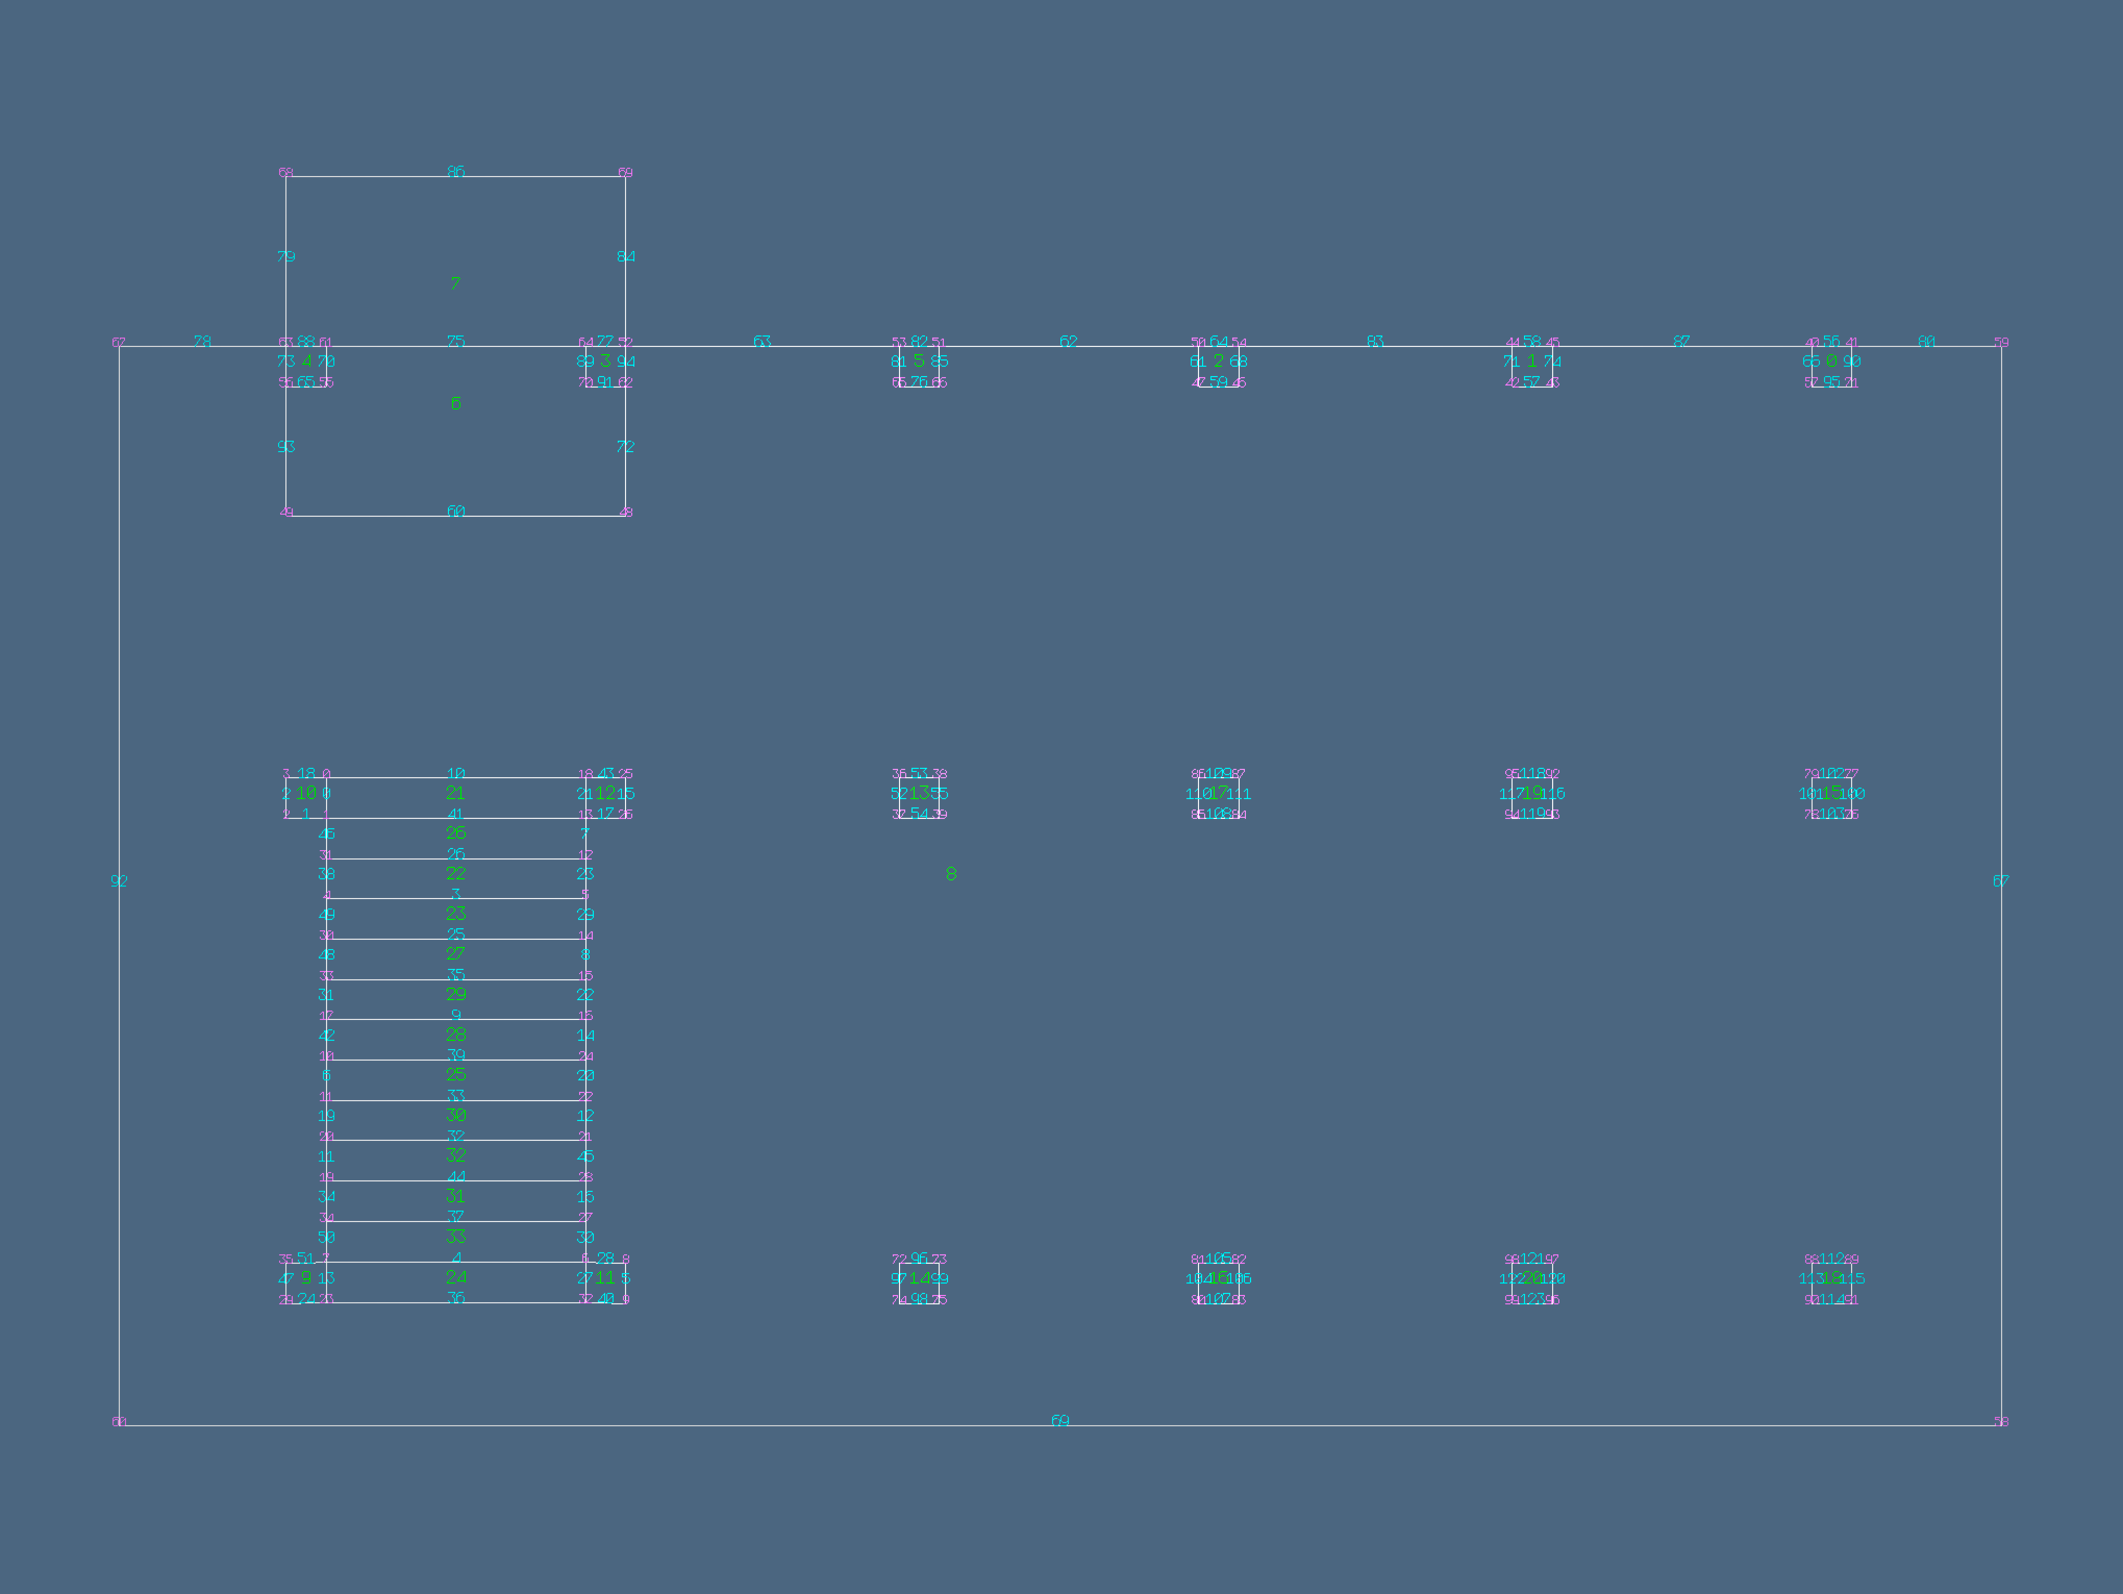
\includegraphics[width=0.495\linewidth]{images/floor1} 
   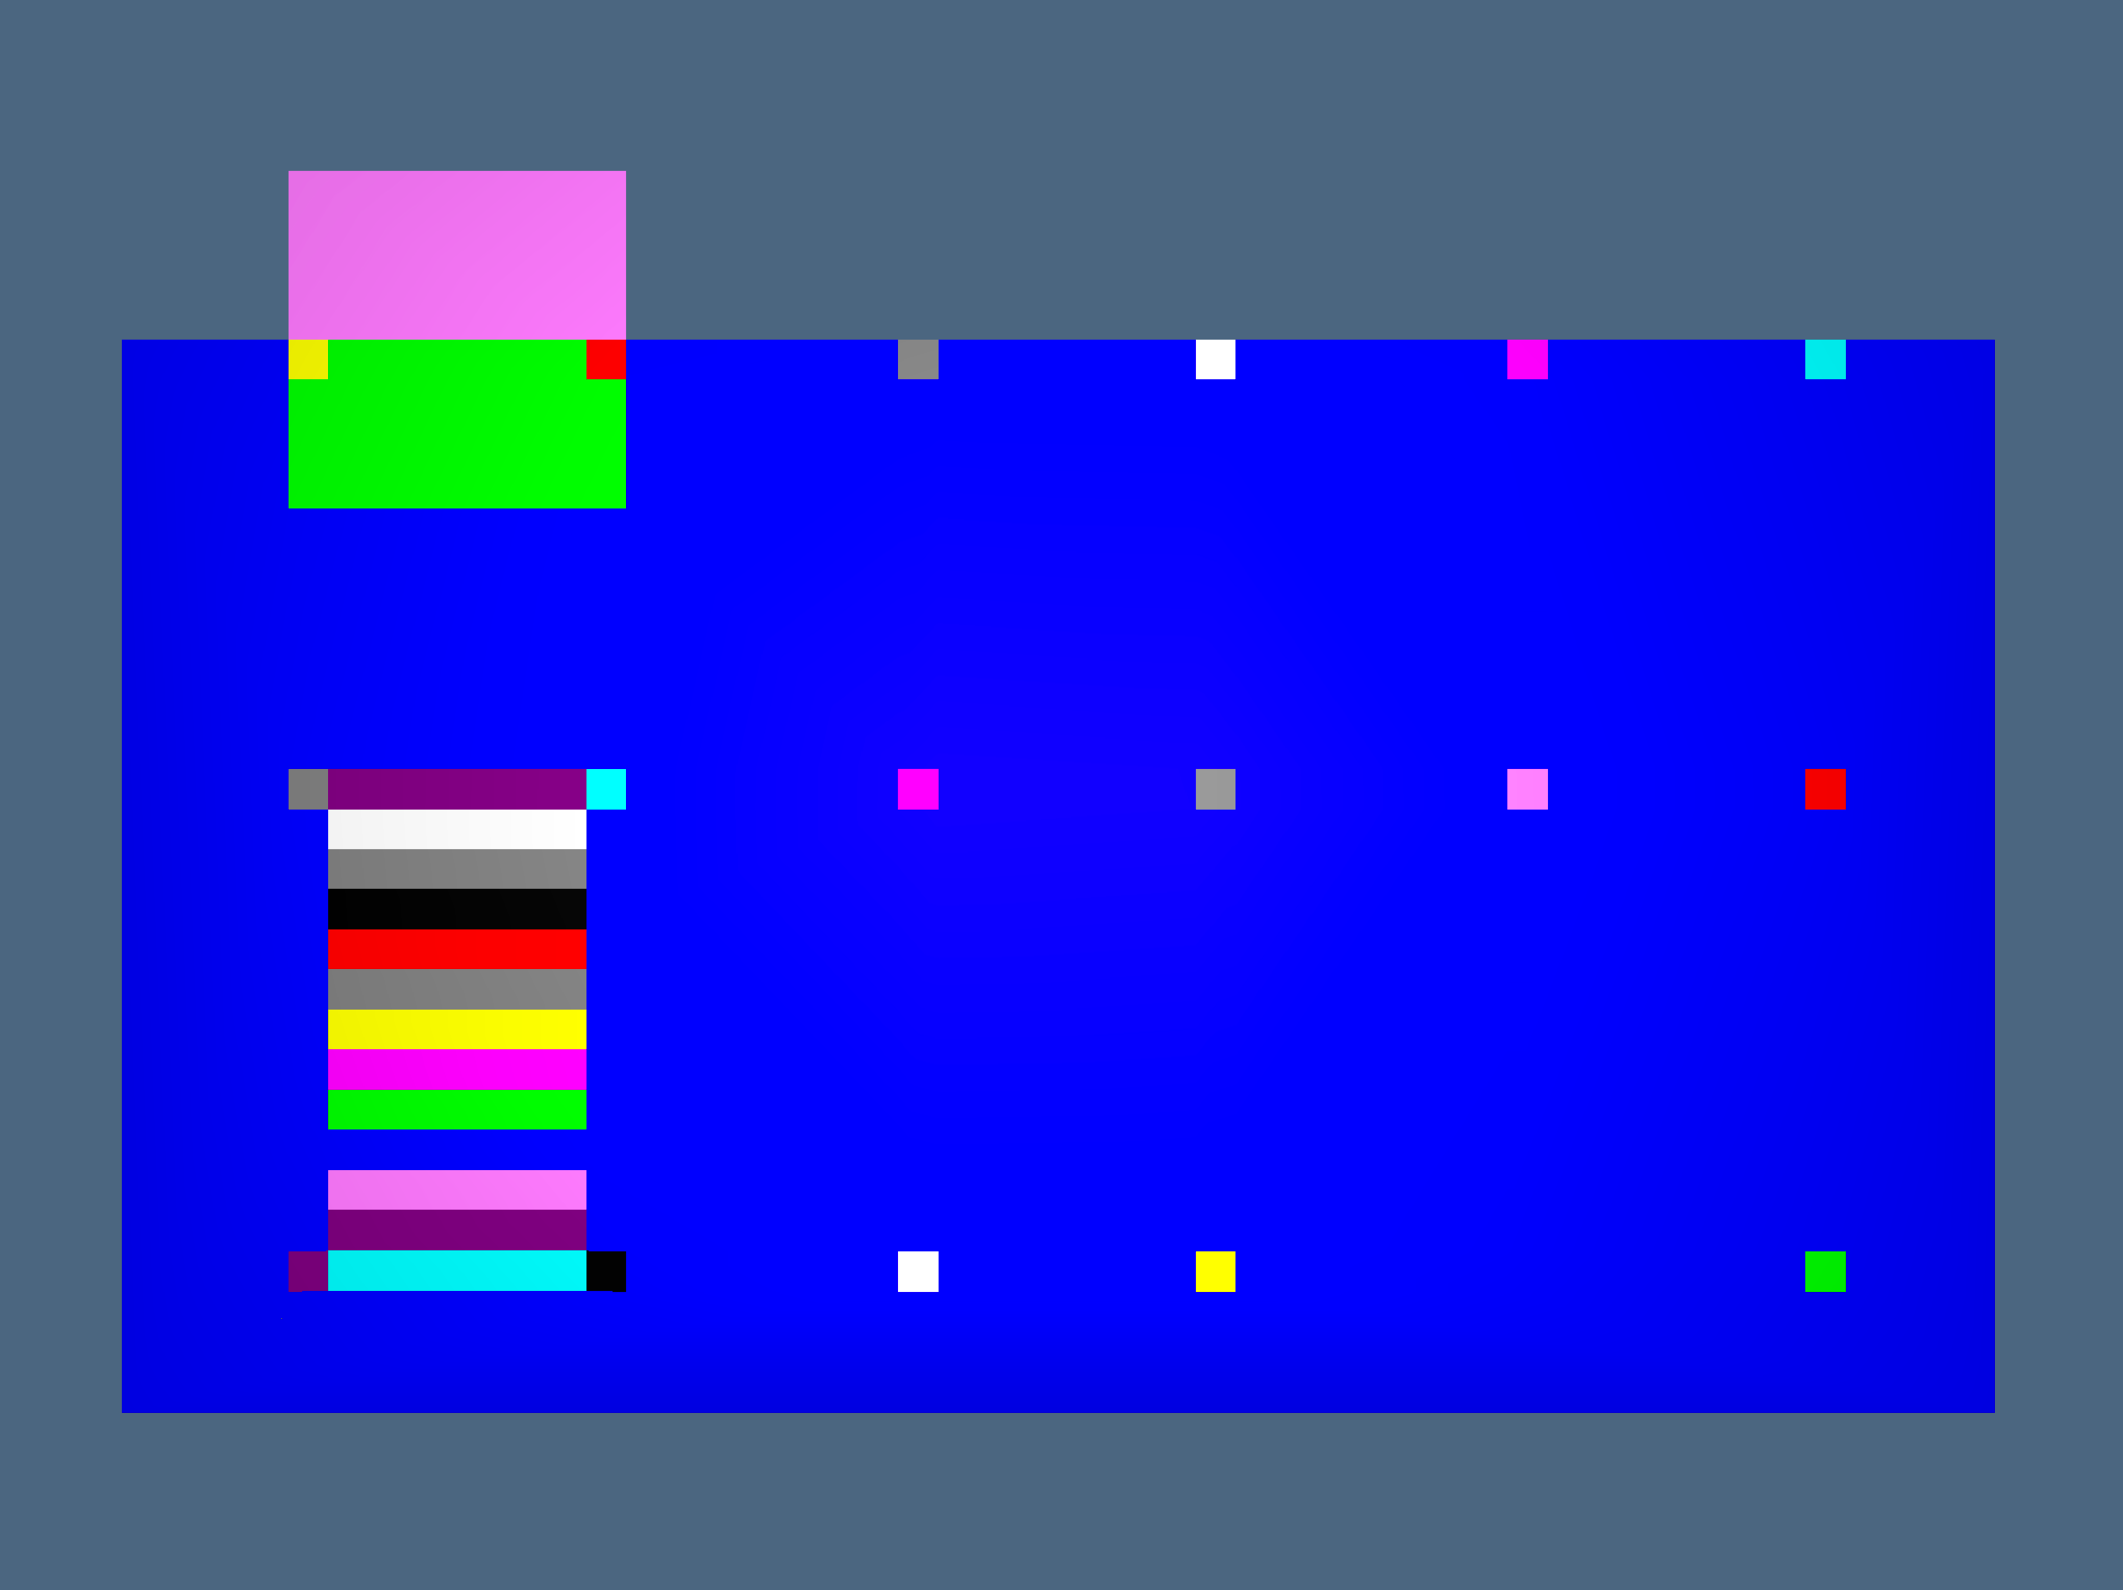
\includegraphics[width=0.495\linewidth]{images/floor2} 

   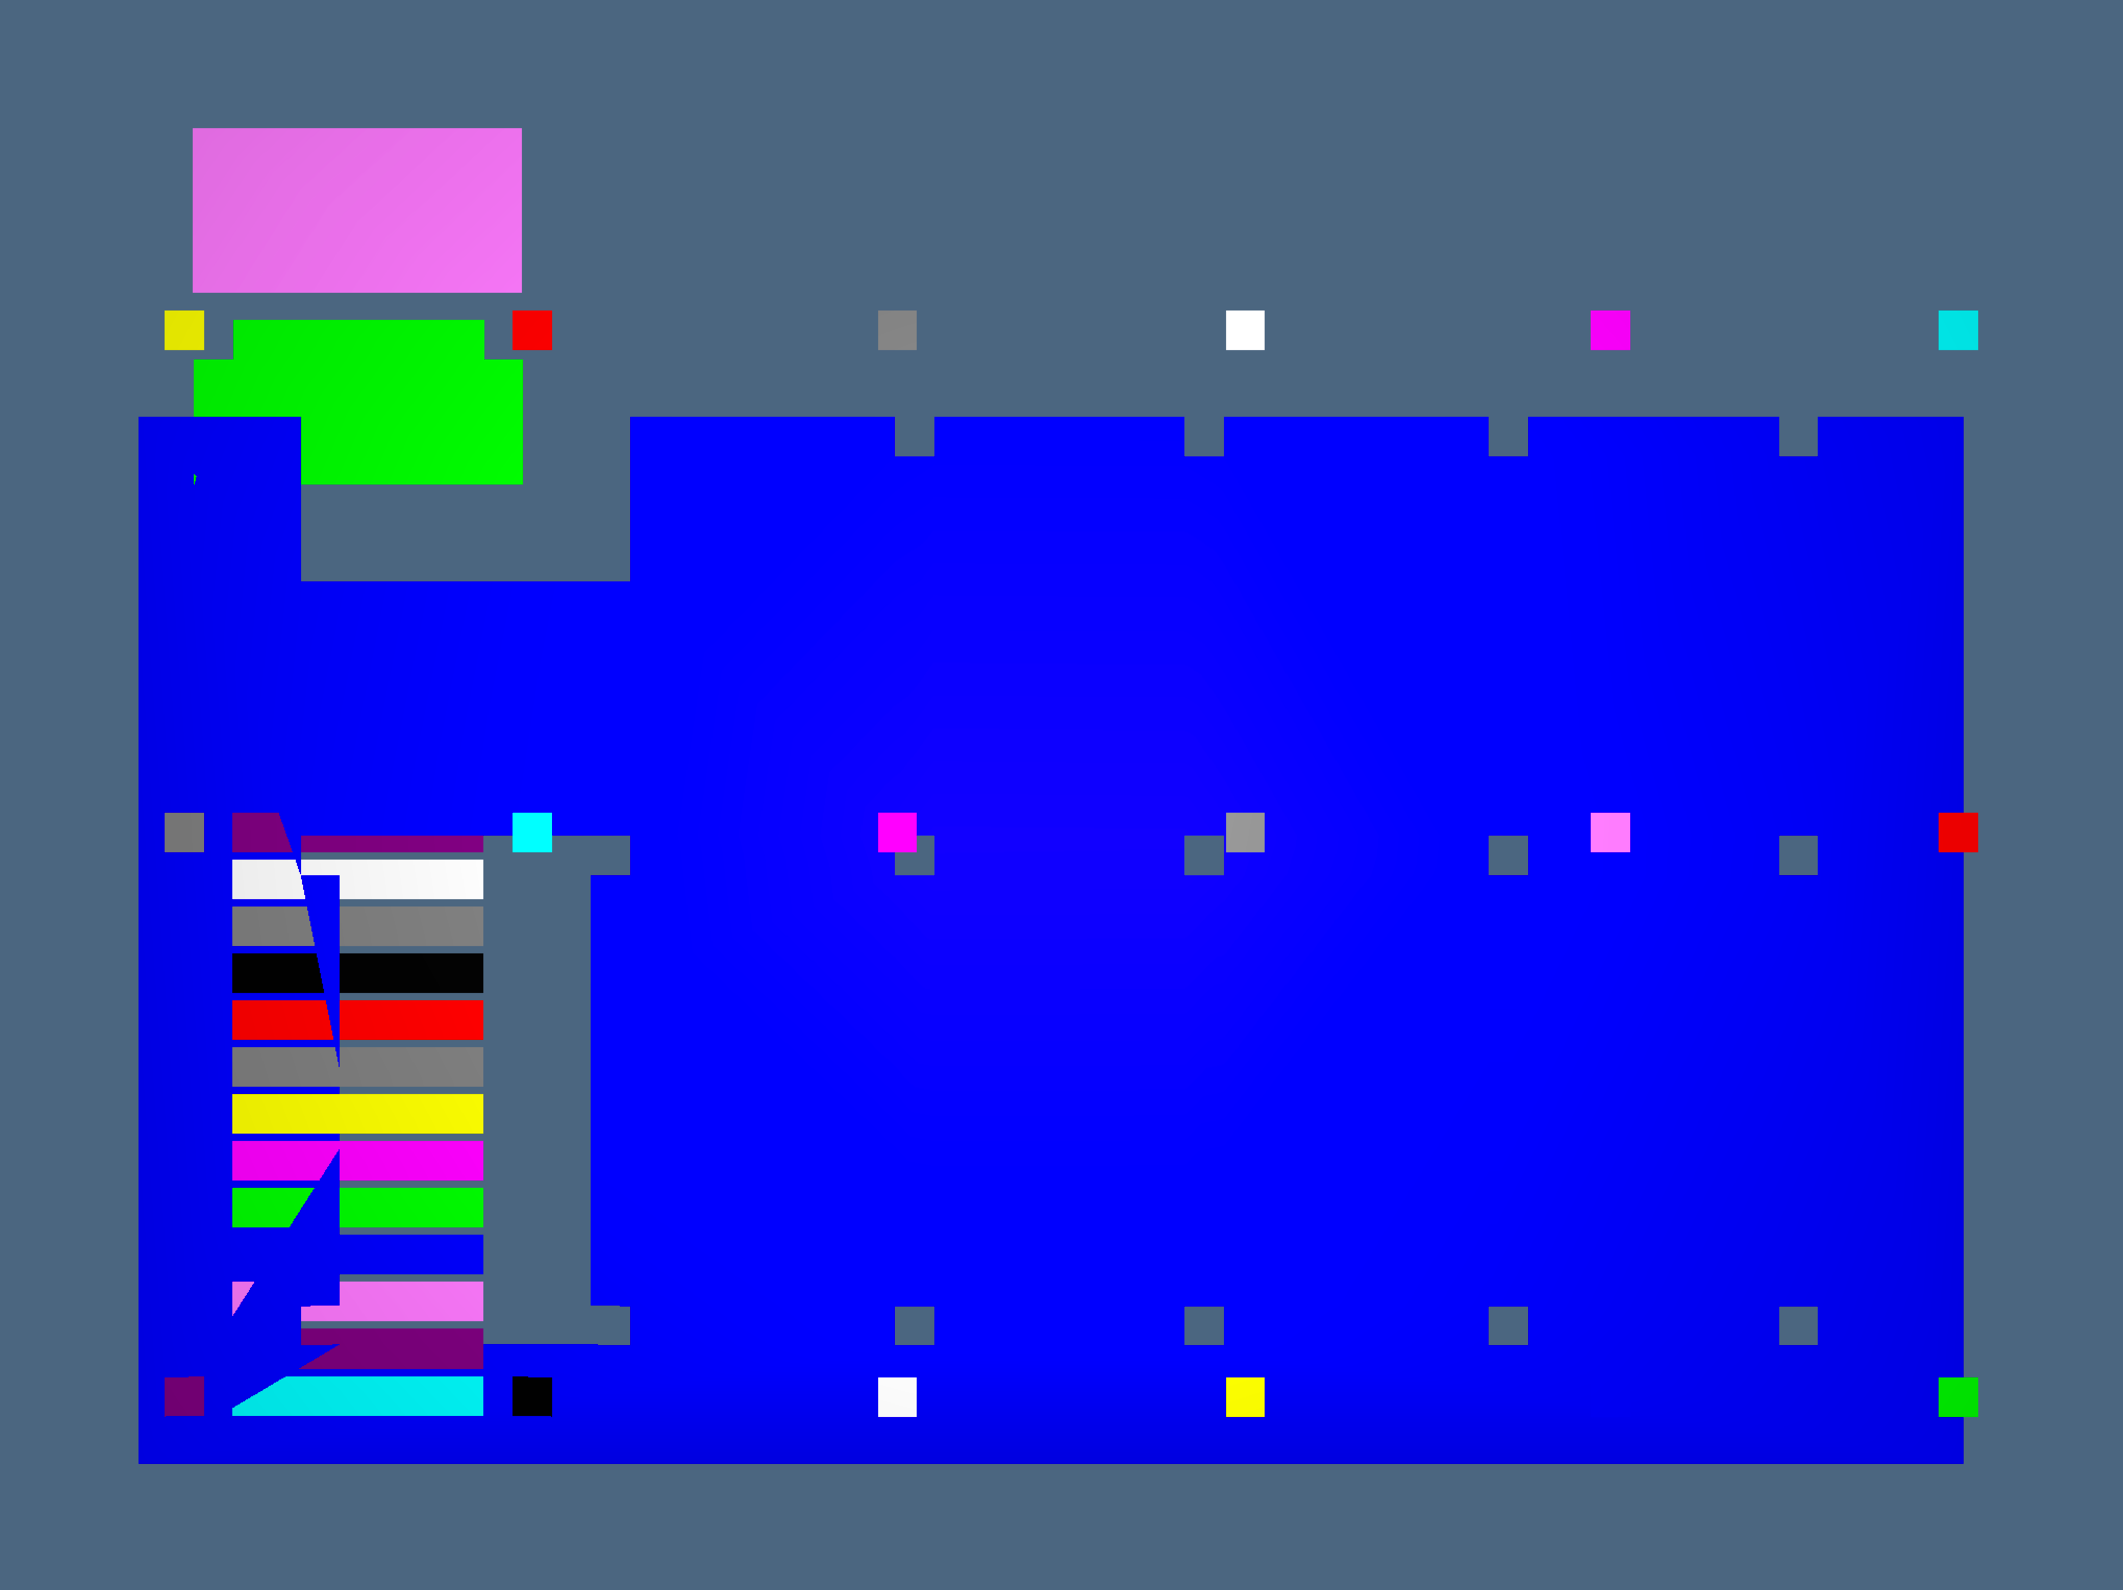
\includegraphics[width=0.495\linewidth]{images/floor3} 
   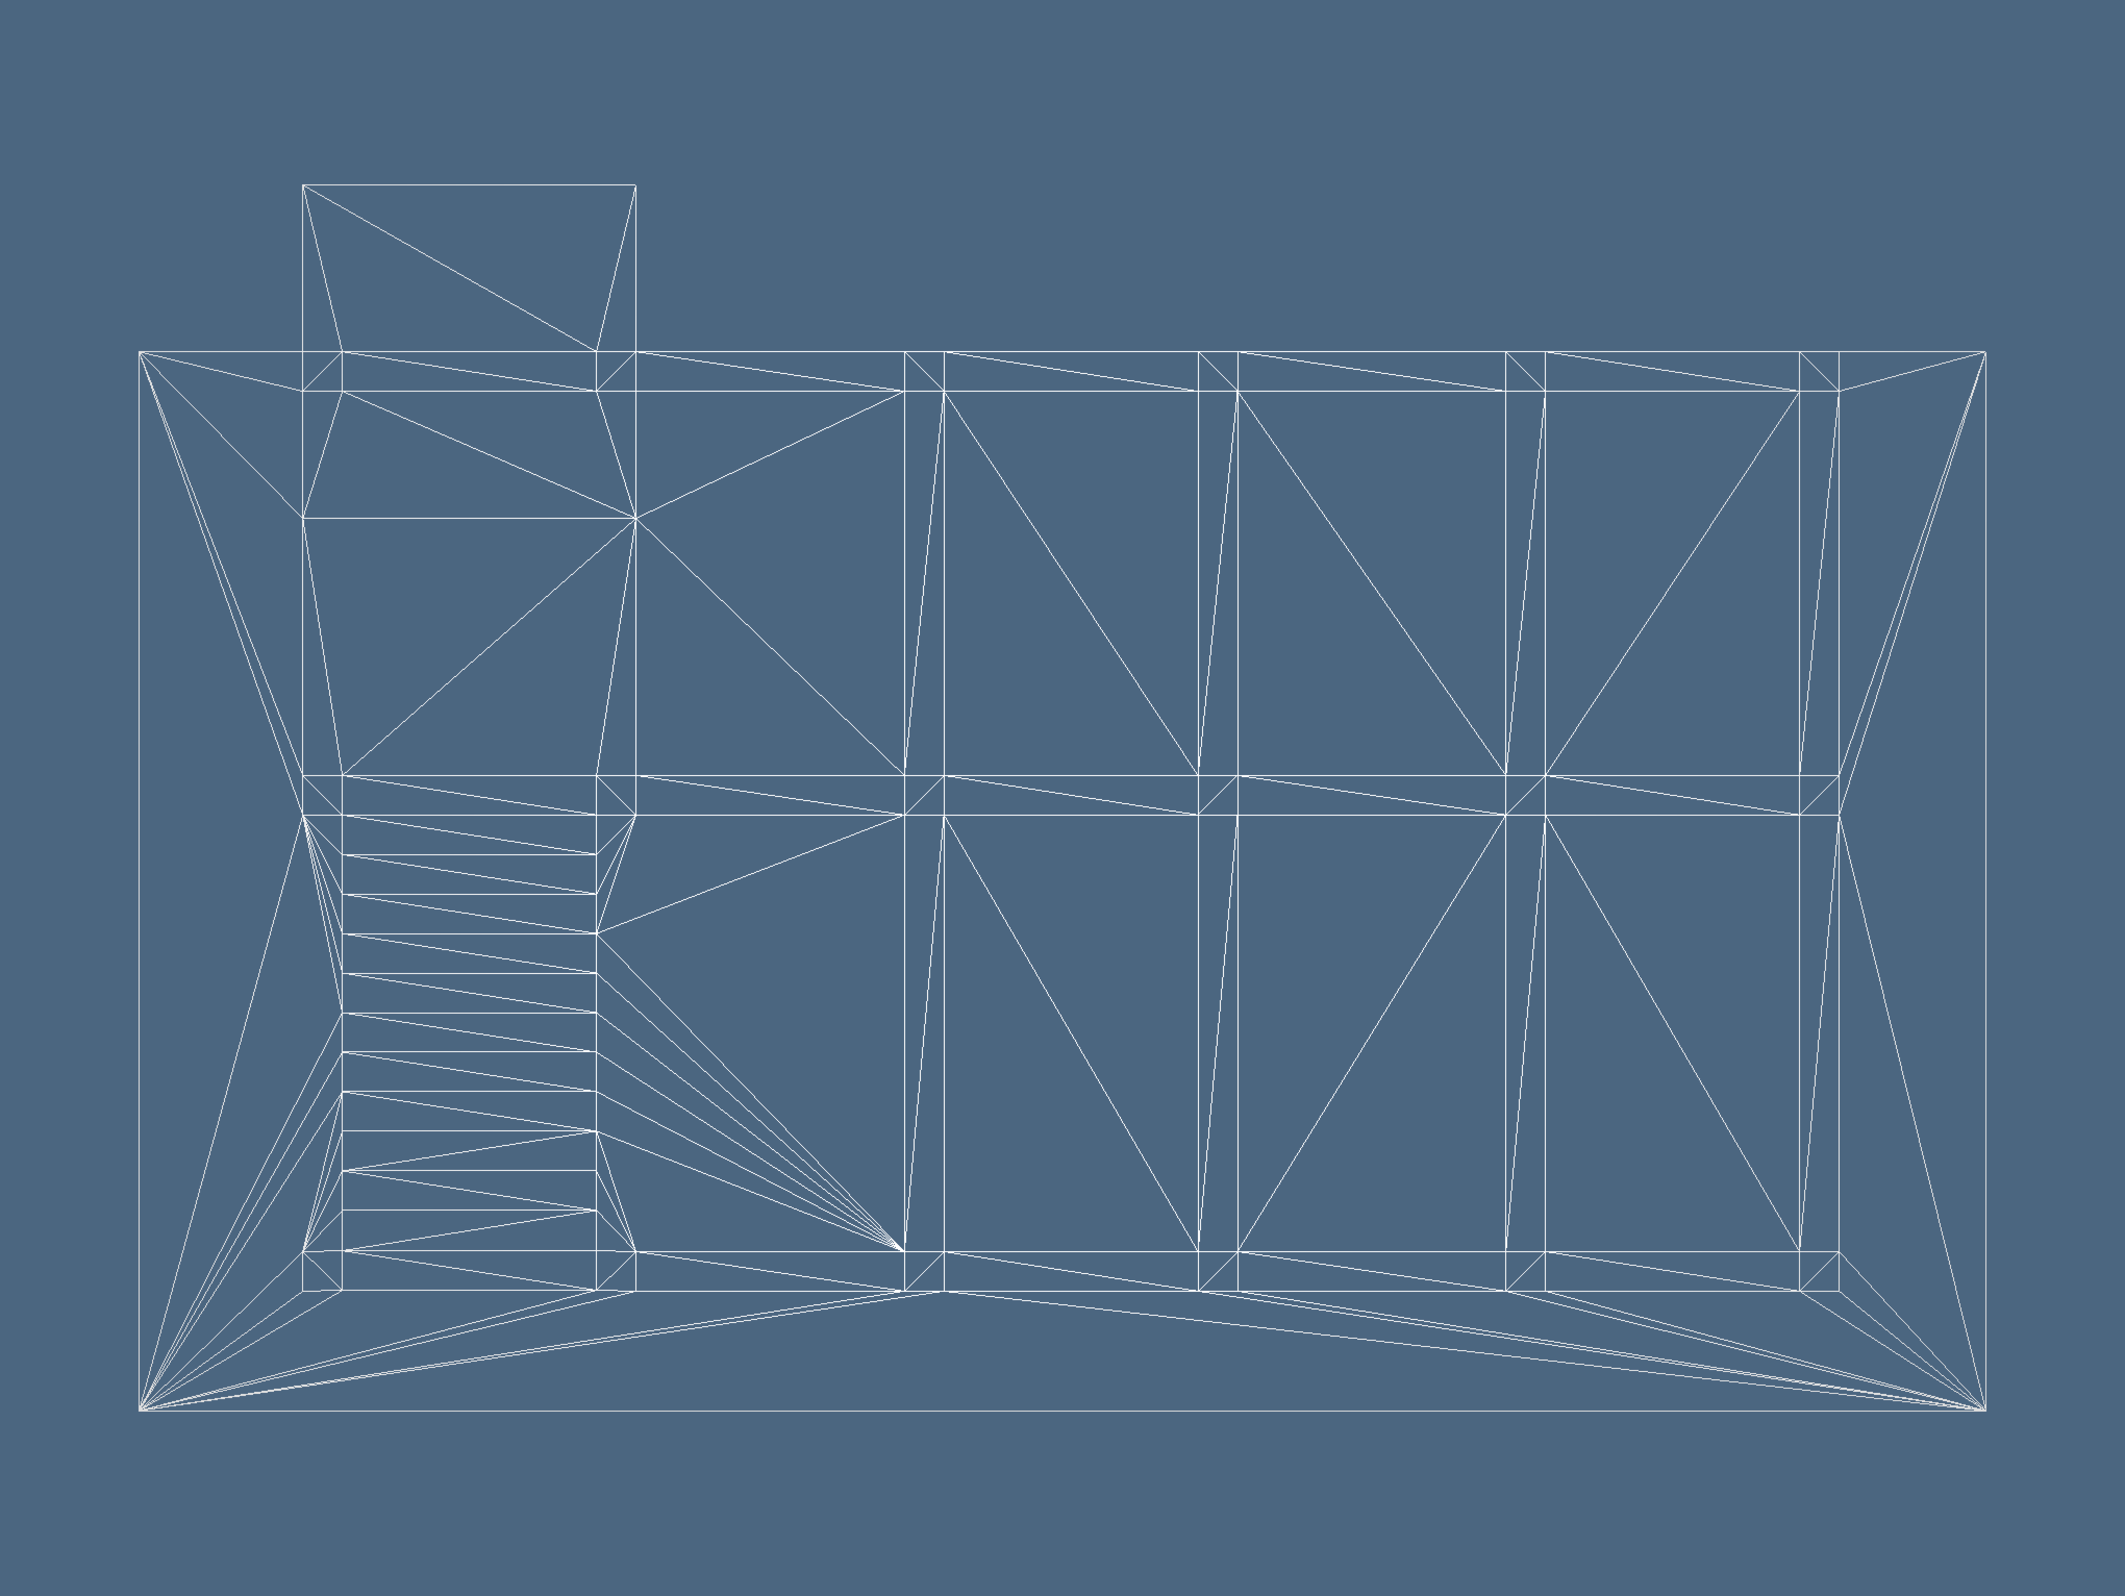
\includegraphics[width=0.495\linewidth]{images/floor4} 
   \caption{Example of LAR 2-complex with non-reducible cells: (a)  the numbering of cells after the generation of the LAR model triple \texttt{(V,FV,EV)} after the input of the \texttt{.svg} file made of SVG primitives (lines and rectangles, in this case); (b)  rendering of the reconstructed 2-complex with non-reducible cells, with one-to-one color rendering of 2-cells; (c)  exploded image of the 2-complex. Notice the holes in the blue cell; (d)  CDT (constrained Delaunay triangulation) of the 2-cells of the complex.}
   \label{fig:floor}
\end{figure}

@D The LAR model triple shown in Figure~\ref{fig:floor}
@{
V =[[0.1101,0.6804],[0.1101,0.659],[0.0887,0.659],[0.0887,0.6804],[0.1101,0.6162],[0.2477,
0.6162],[0.2477,0.4231],[0.1101,0.4231],[0.2691,0.4226],[0.2691,0.4012],[0.1101,0.5306],[0
.1101,0.5092],[0.2477,0.6376],[0.2477,0.659],[0.2477,0.5948],[0.2477,0.5734],[0.2477,0.552
],[0.1101,0.552],[0.2477,0.6804],[0.1101,0.4663],[0.1101,0.4878],[0.2477,0.4878],[0.2477,0
.5092],[0.1101,0.4017],[0.2477,0.5306],[0.2691,0.6804],[0.2691,0.659],[0.2477,0.4449],[0.
2477,0.4663],[0.0887,0.4012],[0.1101,0.5948],[0.1101,0.6376],[0.2477,0.4017],[0.1101,0.
5734],[0.1101,0.4449],[0.0887,0.4226],[0.4144,0.6804],[0.4144,0.659],[0.4358,0.6804],[0.
4358,0.659],[0.8991,0.9098],[0.9205,0.9098],[0.7401,0.8884],[0.7615,0.8884],[0.7401,0.9098
],[0.7615,0.9098],[0.5948,0.8884],[0.5734,0.8884],[0.2691,0.8196],[0.0887,0.8196],[0.5734,
0.9098],[0.4358,0.9098],[0.2691,0.9098],[0.4144,0.9098],[0.5948,0.9098],[0.1101,0.8884],[0
.0887,0.8884],[0.8991,0.8884],[1.0,0.3364],[1.0,0.9098],[0.0,0.3364],[0.1101,0.9098],[0.
2691,0.8884],[0.0887,0.9098],[0.2477,0.9098],[0.4144,0.8884],[0.4358,0.8884],[0.0,0.9098],
[0.0887,1.0],[0.2691,1.0],[0.2477,0.8884],[0.9205,0.8884],[0.4144,0.4226],[0.4358,0.4226],
[0.4144,0.4012],[0.4358,0.4012],[0.9205,0.659],[0.9205,0.6804],[0.8991,0.659],[0.8991,0.
6804],[0.5734,0.4012],[0.5734,0.4226],[0.5948,0.4226],[0.5948,0.4012],[0.5948,0.659],[0.
5734,0.659],[0.5734,0.6804],[0.5948,0.6804],[0.8991,0.4226],[0.9205,0.4226],[0.8991,0.4012
],[0.9205,0.4012],[0.7615,0.6804],[0.7615,0.659],[0.7401,0.659],[0.7401,0.6804],[0.7615,0.
4012],[0.7615,0.4226],[0.7401,0.4226],[0.7401,0.4012]]

FV =[[40,41,71,57],[42,43,44,45],[50,54,46,47],[64,52,62,70],[56,63,61,55],[65,66,51,53],[
64,70,48,49,55,56,61,62],[64,68,69,52,61,63],[0,1,2,3,4,5,6,7,8,9,10,11,12,13,14,15,16,17,
18,19,20,21,22,23,24,25,26,27,28,29,30,31,32,33,34,35,36,37,38,39,40,41,42,43,44,45,46,47,
48,49,50,51,52,53,54,56,57,58,59,60,62,63,65,66,67,71,72,73,74,75,76,77,78,79,80,81,82,83,
84,85,86,87,88,89,90,91,92,93,94,95,96,97,98,99],[35,7,29,23],[0,1,2,3],[8,9,6,32],[25,26,
18,13],[36,37,38,39],[72,73,74,75],[76,77,78,79],[80,81,82,83],[84,85,86,87],[88,89,90,91]
,[92,93,94,95],[96,97,98,99],[0,1,18,13],[12,4,5,31],[14,4,5,30],[32,23,6,7],[24,10,11,22]
,[1,12,13,31],[33,30,14,15],[16,17,10,24],[16,17,33,15],[11,20,21,22],[19,34,27,28],[28,19
,20,21],[34,27,6,7]]

EV=[[0,1],[1,2],[3,2],[4,5],[6,7],[8,9],[10,11],[12,13],[14,15],[16,17],[0,18],[19,20],[21
,22],[23,7],[24,16],[25,26],[27,28],[26,13],[3,0],[11,20],[24,22],[13,18],[15,16],[5,12],[
29,23],[14,30],[12,31],[6,32],[6,8],[14,5],[6,27],[17,33],[20,21],[11,22],[34,19],[15,33],
[32,23],[27,34],[4,31],[24,10],[32,9],[1,13],[10,17],[25,18],[19,28],[28,21],[31,1],[29,35
],[33,30],[4,30],[34,7],[35,7],[36,37],[36,38],[39,37],[38,39],[40,41],[42,43],[44,45],[46
,47],[48,49],[50,47],[50,51],[52,53],[54,50],[55,56],[40,57],[58,59],[54,46],[58,60],[55,
61],[42,44],[62,48],[56,63],[45,43],[61,64],[65,66],[52,64],[63,67],[68,63],[41,59],[65,53
],[53,51],[54,44],[69,52],[66,51],[68,69],[45,40],[63,61],[70,64],[41,71],[62,70],[60,67],
[56,49],[52,62],[57,71],[72,73],[74,72],[75,74],[75,73],[76,77],[78,79],[79,77],[76,78],[
80,81],[81,82],[82,83],[80,83],[84,85],[86,87],[86,85],[87,84],[88,89],[90,88],[91,90],[91
,89],[92,93],[94,95],[92,95],[93,94],[96,97],[97,98],[99,98],[96,99]]@}

\subsection{Monocyclic polygons using bridge-edges}
%~~~~~~~~~~~~~~~~~~~~~~~~~~~~~~~~~~~~~~~~~~~~~~~~~~~~~~~~~~~~~~~~~~~~~~~~~~~~~~~

This subsection, even if correct, is not currently used, since the used triangulation algorithm, from the \texttt{poly2tri} package, cannot handle repeated vertices.

\paragraph{Generation of 1-boundaries as vertex permutation}
In algebraic topology a $k$-cycle is a $k$-chain whose boundary is empty. Also, an unconnected $k$-cycle is the direct sum of two or more $k$-cycles. A good formal representation of every simplicial $k$-cycle, where \emph{each} component $k$-simplex has $k+1$ $(k-1)$-adjacent $k$-simplices is a $(k+1)$-array, indexed by $k$-simplices, i.e.~the \emph{Winged Representation}~\cite{Paoluzzi:1993:DMS:169728.169719}. 

In the case of oriented $1$-cycles, a good representation is given by considering the (ordering of) 0-faces (vertices) as a permutation of $n$ integers, i.e.~as a bijective function $\pi :[0,n]\to[0,n]$ that can be represented as an array \texttt{verts} of integers indexed on integers, and the 1-faces (edges) as a dictionary (mapping) \texttt{nextVert} $verts\to verts$.

In order to join two component cycles using one of \texttt{bridgeEdges}, say $(u,v)$, computed by the function \texttt{connectTheDots} previously given, we must save $\pi(u)$ and $\pi(v)$, say, within $x$ and $y$, respectively
%-------------------------------------------------------------------------------
@D Generation of 1-boundaries as vertex permutation 
@{""" Generation of 1-boundaries as vertex permutation """
def boundaryCycles2vertexPermutation( model ):
    V,EV = model
    cells,bridgeEdges = connectTheDots(model)
    CVs = orientBoundaryCycles(model,cells)
    
    verts = CAT(CAT( CVs ))
    n = len(verts)
    W = copy.copy(V)
    #assert len(verts) == sorted(verts)[n-1]-sorted(verts)[0]+1
    nextVert = dict([(v,cycle[(k+1)%(len(cycle))]) for cell in CVs for cycle in cell 
                   for k,v in enumerate(cycle)])
    for k,(u,v) in enumerate(CAT(bridgeEdges)):
        x,y = nextVert[u],nextVert[v]
        nextVert[u] = n+2*k+1
        nextVert[v] = n+2*k      
        nextVert[n+2*k] = x
        nextVert[n+2*k+1] = y
        W += [W[u]]
        W += [W[v]]
        EW = nextVert.items()
    return W,EW
@}
%-------------------------------------------------------------------------------

\paragraph{Wire-frame LAR to boundary polygons}
The 2-dimensional LAR model \texttt{(W,EW)} returned by the function \texttt{boundaryCycles2vertexPermutation} is pretty special, since it is at the same time both a standard LAR model, i.e.~a pair (vertices, edges\_by\_vertices), and a permutation of vertex indices providing implicitly the ordered cycles on the boundary of a 2-complex. In other words, \texttt{EW} is both a (possibly unconnected) 1-cycle and an 1-boundary.

In the following script we extract the list of connected boundaries (including bridge-edges) from the \texttt{EW} permutation of the first $m$ integers.

%-------------------------------------------------------------------------------
@D Wire-frame LAR to boundary polygons 
@{""" lar2boundaryPolygons """
def lar2boundaryPolygons(model):
    W,EW = boundaryCycles2vertexPermutation( model )
    EW = AA(list)(EW)
    polygons = []
    for k,edge in enumerate(EW):
        polygon = []
        if edge[0]>=0:
            first = edge[0]
            done = False
        while (not done) and edge[0] >= 0:
            polygon += [edge[0]]
            edge[0] = -edge[0]
            edge = EW[edge[1]]
            if len(polygon)>1 and polygon[-1] == first: 
                EW[first][0] = -float(first)
                break 
        if polygon != []: 
            if polygon[0]==polygon[-1]: polygon=polygon[:-1]
            polygons += [polygon]
    return W,polygons
@}       
%-------------------------------------------------------------------------------

\begin{figure}[htbp] %  figure placement: here, top, bottom, or page
   \centering
   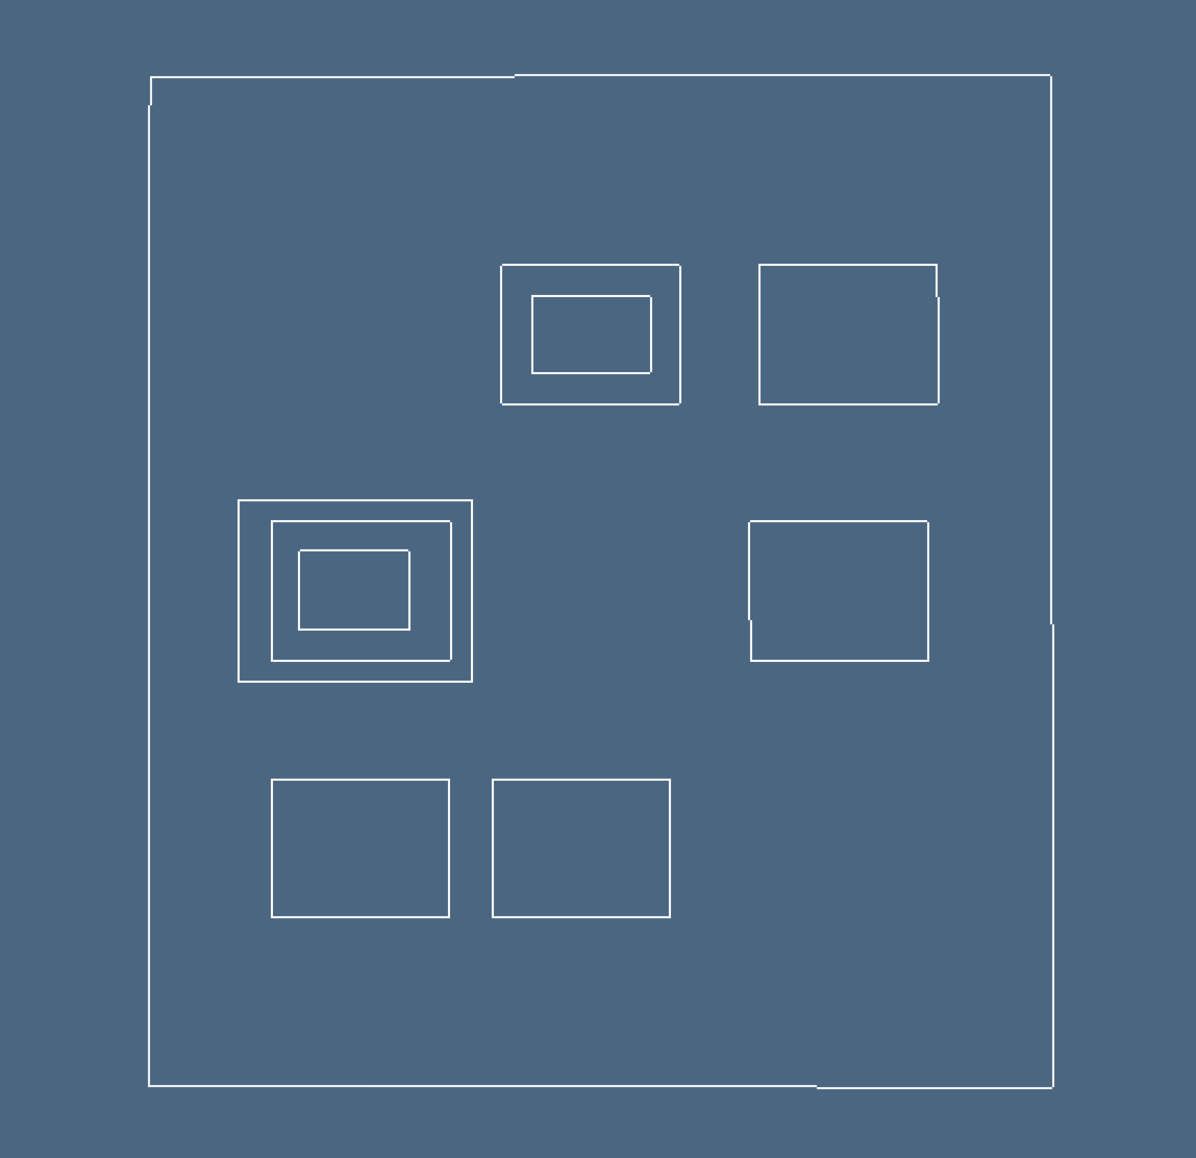
\includegraphics[height=0.32\linewidth,width=0.32\linewidth]{images/holes1}
   
\includegraphics[height=0.32\linewidth,width=0.32\linewidth]{images/holes3} 
   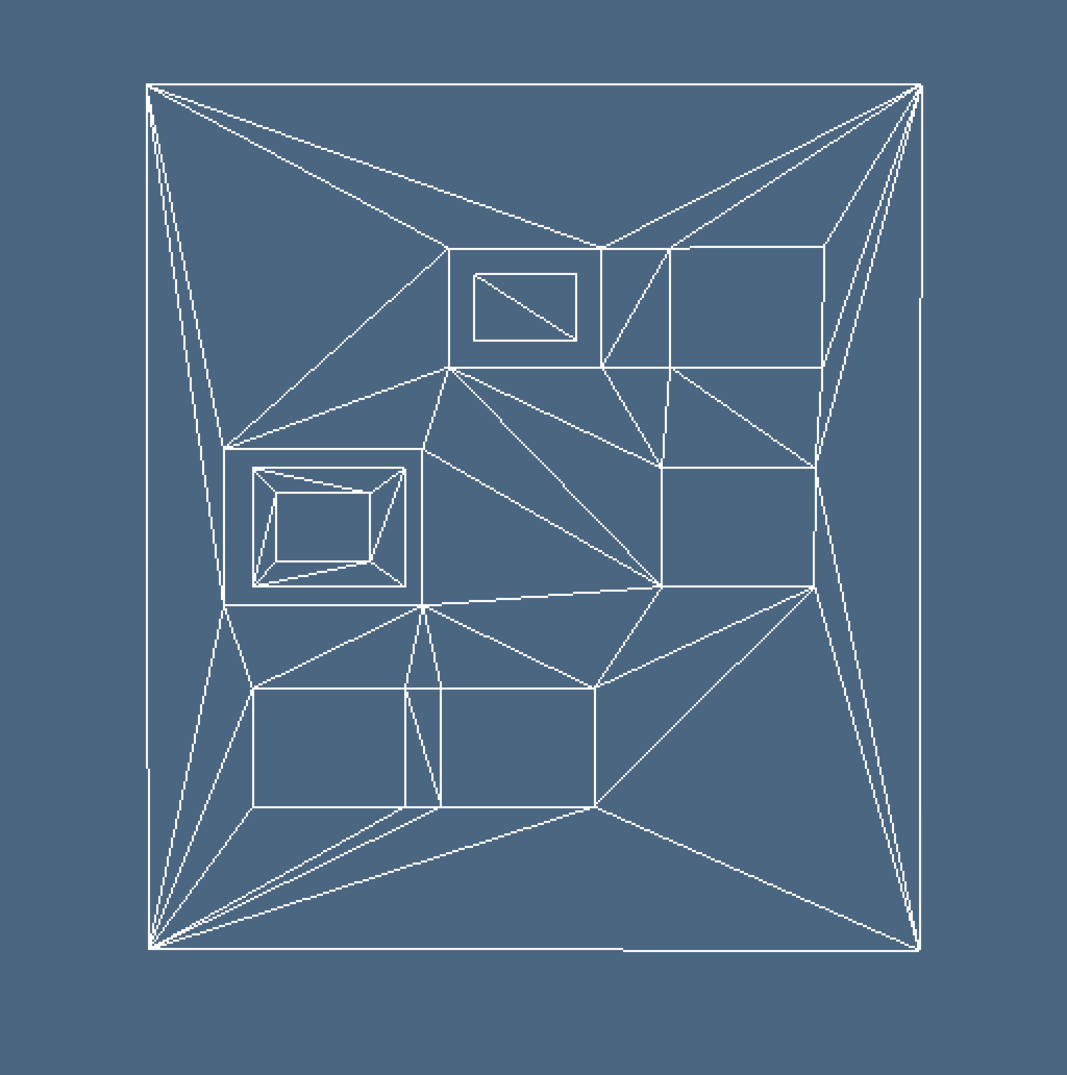
\includegraphics[height=0.32\linewidth,width=0.32\linewidth]{images/holes2} 
   \caption{(a) Closed 1-chain $c$, i.e.~such that $\partial\, c = 0$; $c$ is both cycle and boundary at the same time; (b) 2-chain $h$ such that $\partial\,h = c$; (c) 1-skeleton of a triangulation of $h$.}
   \label{fig:cycles}
\end{figure}


\paragraph{Edge cycles associated to a closed chain of edges}

The output \texttt{cycles} are returned as lists of oriented edges, given in consecutive  sequence in each list. Each cycle is given in the opposite ordering of its first edge.
The first edge of each cycle is the one of minimum index in the cycle. The list of output cycles is returned ordered for increasing (or better, in decreasing order, since negative) order of its first element. The first output cycle starts from index 0, that cannot oriented directly, since -0 is not allowed for integer indices. It must be considered as negative, i.e. as oriented as the opposite of its canonical orientation. 

%-------------------------------------------------------------------------------
@D Edge cycles associated to a closed chain of edges
@{""" Edge cycles associated to a closed chain of edges """

from collections import defaultdict

def detachManifolds(polygonVerts):
    vertCycles = []
    for vertexList in polygonVerts:
        vertCount,counts = defaultdict(list),list
        for v in vertexList: 
            vertCount[v] += [1]
        counts = [sum(vertCount[v]) for v in vertexList]
        vertCycles += [counts]
    return vertCycles
    
def splitManifolds(cycles,vertices,manifolds):
    out = []
    for cycle,verts,manifold in zip(cycles,vertices,manifolds):
        if sum(manifold) == len(manifold):
            out += [cycle] 
        else:
            transpositionNumbers = [n for n,k in enumerate(manifold) if k>1]
            n = transpositionNumbers[0]
            cycle = rotatePermutation(cycle,n) 
            verts = rotatePermutation(verts,n) 
            manifold = rotatePermutation(manifold,n) 
            starts = AA(C(sum)(-n))(transpositionNumbers)+[len(manifold)]
            pairs = [(start,starts[k+1]) for k,start in enumerate(starts[:-1])]
            splitCycles = [[cycle[k] for k in range(*interval)] for interval in pairs]
            splitVerts = [[verts[k] for k in range(*interval)] for interval in pairs]
            out += splitCycles
    return out

def boundaryCycles(edgeBoundary,EV):
    cycles,cycle = [],[]
    vertices = []
    
    def singleBoundaryCycle(edgeBoundary):
        verts2edges = defaultdict(list)
        for e in edgeBoundary:
            verts2edges[EV[e][0]] += [e]
            verts2edges[EV[e][1]] += [e]
        cycle,verts = [],[]
        
        if edgeBoundary == []: return cycle,verts
        e = edgeBoundary[0]
        v,w = EV[e]
        verts = [v,w]
        while edgeBoundary != []:
            cycle += [e]
            edgeBoundary.remove(e)
            v,w = EV[e]
            verts2edges[v].remove(e)
            verts2edges[w].remove(e)
            w = list(set(EV[e]).difference([verts[-1]]))[0]
            if verts2edges[w] == []: break
            e = verts2edges[w][0]
            verts += [w]
        verts = verts[1:]
        return cycle,verts
        
    while edgeBoundary != []:
        edgeBoundary = list(set(edgeBoundary).difference(cycle))
        cycle,verts = singleBoundaryCycle(edgeBoundary)
        if cycle!= []: 
            cycle = [e if verts[k]==EV[e][0] else -e for k,e in enumerate(cycle)]
            cycles += [cycle]
            vertices += [verts]
    manifolds = detachManifolds(vertices)
    cycles = splitManifolds(cycles,vertices,manifolds)
    return cycles,vertices
@}
%-------------------------------------------------------------------------------



\paragraph{From Struct object to LAR boundary model}
%-------------------------------------------------------------------------------
@D From Struct object to LAR boundary model
@{""" From Struct object to LAR boundary model """
def structFilter(obj):
    if isinstance(obj,list):
        if (len(obj) > 1):
            return [structFilter(obj[0])] + structFilter(obj[1:])
        return [structFilter(obj[0])]
    if isinstance(obj,Struct):
        if obj.category in ["external_wall", "internal_wall", "corridor_wall"]:
            return
        return Struct(structFilter(obj.body),obj.name,obj.category)
    return obj

import boundary

def structBoundaryModel(struct):
    filteredStruct = structFilter(struct)
    #import pdb; pdb.set_trace()
    V,FV,EV = struct2lar(filteredStruct)
    edgeBoundary = boundary.boundaryCells(FV,EV)
    cycles,_ = boundaryCycles(edgeBoundary,EV)
    edges = [signedEdge for cycle in cycles for signedEdge in cycle]
    orientedBoundary = [ AA(SIGN)(edges), AA(ABS)(edges)]
    cells = [EV[e] if sign==1 else REVERSE(EV[e]) for (sign,e) in zip(*orientedBoundary)]
    if cells[0][0]==cells[1][0]: # bug badly patched! ... TODO better
        temp0 = cells[0][0]
        temp1 = cells[0][1]
        cells[0] = [temp1, temp0]
    return V,cells
@}
%-------------------------------------------------------------------------------



\paragraph{From structures to boundary polylines}
Notice that the \texttt{if} predicate \texttt{len(V) < len(boundaryEdges)} 
is used to discriminate between manifold (\texttt{False}) and non-manifold (\texttt{True})
boundary cases.
%-------------------------------------------------------------------------------
@D From structures to boundary polylines
@{""" From structures to boundary polylines """
def boundaryPolylines(struct):
    V,boundaryEdges = structBoundaryModel(struct)
    if len(V) < len(boundaryEdges):
        EV = AA(sorted)(boundaryEdges)
        boundaryEdges = range(len(boundaryEdges))
        cycles,vertices = boundaryCycles(boundaryEdges,EV)
        polylines = [[V[v] for v in verts]+[V[verts[0]]] for verts in REVERSE(vertices)]
    else:
        polylines = boundaryModel2polylines((V,boundaryEdges))
    return polylines
@}
%-------------------------------------------------------------------------------


\paragraph{From LAR oriented boundary model to polylines}
%-------------------------------------------------------------------------------
@D From LAR boundary model to polylines
@{""" From LAR oriented boundary model to polylines """
def boundaryModel2polylines(model):
    if len(model)==2: V,EV = model
    elif len(model)==3: V,FV,EV = model
    polylines = []
    succDict = dict(EV)
    visited = [False for k in range(len(V))]
    nonVisited = [k for k in succDict.keys() if not visited[k]]
    while nonVisited != []:
        first = nonVisited[0]; v = first; polyline = []
        while visited[v] == False:
            visited[v] = True; 
            polyline += V[v], 
            v = succDict[v]
        polyline += [V[first]]
        polylines += [polyline]
        nonVisited = [k for k in succDict.keys() if not visited[k]]
    return polylines

def boundaryModel2polylines(model):
    if len(model)==2: V,EV = model
    elif len(model)==3: V,FV,EV = model
    polylines = []
    succDict = dict(EV)
    visited = [False for k in range(len(V))]
    nonVisited = [k for k in succDict.keys() if not visited[k]]
    while nonVisited != []:
        first = nonVisited[0]; v = first; polyline = []
        while visited[v] == False:
            visited[v] = True; 
            polyline += V[v], 
            v = succDict[v]
        polyline += [V[first]]
        polylines += [polyline]
        nonVisited = [k for k in succDict.keys() if not visited[k]]
    return polylines
@}
%-------------------------------------------------------------------------------





\subsection{Visualization of a 2D complex and 2-chain}

%-------------------------------------------------------------------------------
@D Visualization of a 2D complex and 2-chain
@{""" Visualization of a 2D complex and 2-chain """
def larComplexChain(model):
    V,FV,EV = model
    VV = AA(LIST)(range(len(V)))
    #csrBoundaryMat = boundary1(FV,EV,VV)
    csrBoundaryMat = boundary.boundary(FV,EV)
    def larComplexChain0(chain):
        boundaryChain = chain2BoundaryChain(csrBoundaryMat)(chain)
        outModel = V,[EV[e] for e in boundaryChain]
        triangleSet = larTriangulation(outModel)
        return boundaryChain,triangleSet
    return larComplexChain0
    
def viewLarComplexChain(model):
    V,FV,EV = model
    operator = larComplexChain(model)
    def viewLarComplexChain0(chain):
        boundaryChain,triangleSet = operator(chain)
        hpcChain = AA(JOIN)(AA(AA(MK))(CAT(triangleSet)))
        hpcChainBoundary = AA(COLOR(RED))(MKPOLS((V,[EV[e] for e in boundaryChain])))
        VIEW(STRUCT( hpcChain + hpcChainBoundary ))
        VIEW(EXPLODE(1.2,1.2,1.2)( hpcChain + hpcChainBoundary ))
    return viewLarComplexChain0
@}
%-------------------------------------------------------------------------------




\subsection{Point in polygon classification}


%-------------------------------------------------------------------------------
@D Point in polygon testing
@{""" Point-in-polygon classification algorithm """
@< Half-line crossing test @>
@< Tile codes computation @>
@< Point-in-polygon classification algorithm @>
@}
%-------------------------------------------------------------------------------

\paragraph{Tile codes computation}
%-------------------------------------------------------------------------------
@D Tile codes computation
@{""" Tile codes computation """
def setTile(box):
    tiles = [[9,1,5],[8,0,4],[10,2,6]]
    b1,b2,b3,b4 = box
    def tileCode(point):
        x,y = point
        code = 0
        if y>b1: code=code|1
        if y<b2: code=code|2
        if x>b3: code=code|4
        if x<b4: code=code|8
        return code 
    return tileCode
@}
%-------------------------------------------------------------------------------


\paragraph{Half-line crossing test}
%-------------------------------------------------------------------------------
@D Half-line crossing test 
@{""" Half-line crossing test """
def crossingTest(new,old,count,status):
    if status == 0:
        status = new
        count += 0.5
    else:
        if status == old: count += 0.5
        else: count -= 0.5
        status = 0
@}
%-------------------------------------------------------------------------------

\paragraph{Point in polygon testing}
%-------------------------------------------------------------------------------
@D Point-in-polygon classification algorithm
@{""" Point in polygon classification """
def pointInPolygonClassification(pol):

    V,EV = pol
    # edge orientation
    FV = [sorted(set(CAT(EV)))]
    orientedCycles = boundaryPolylines(Struct([(V,FV,EV)]))
    EV = []
    for cycle in orientedCycles:
        EV += zip(cycle[:-1],cycle[1:])

    def pointInPolygonClassification0(p):
        x,y = p
        xmin,xmax,ymin,ymax = x,x,y,y
        tilecode = setTile([ymax,ymin,xmax,xmin])
        count,status = 0,0
    
        for k,edge in enumerate(EV):
            p1,p2 = edge[0],edge[1]
            (x1,y1),(x2,y2) = p1,p2
            c1,c2 = tilecode(p1),tilecode(p2)
            c_edge, c_un, c_int = c1^c2, c1|c2, c1&c2
            
            if c_edge == 0 and c_un == 0: return "p_on"
            elif c_edge == 12 and c_un == c_edge: return "p_on"
            elif c_edge == 3:
                if c_int == 0: return "p_on"
                elif c_int == 4: count += 1
            elif c_edge == 15:
                x_int = ((y-y2)*(x1-x2)/(y1-y2))+x2 
                if x_int > x: count += 1
                elif x_int == x: return "p_on"
            elif c_edge == 13 and ((c1==4) or (c2==4)):
                    crossingTest(1,2,status,count)
            elif c_edge == 14 and (c1==4) or (c2==4):
                    crossingTest(2,1,status,count)
            elif c_edge == 7: count += 1
            elif c_edge == 11: count = count
            elif c_edge == 1:
                if c_int == 0: return "p_on"
                elif c_int == 4: crossingTest(1,2,status,count)
            elif c_edge == 2:
                if c_int == 0: return "p_on"
                elif c_int == 4: crossingTest(2,1,status,count)
            elif c_edge == 4 and c_un == c_edge: return "p_on"
            elif c_edge == 8 and c_un == c_edge: return "p_on"
            elif c_edge == 5:
                if (c1==0) or (c2==0): return "p_on"
                else: crossingTest(1,2,status,count)
            elif c_edge == 6:
                if (c1==0) or (c2==0): return "p_on"
                else: crossingTest(2,1,status,count)
            elif c_edge == 9 and ((c1==0) or (c2==0)): return "p_on"
            elif c_edge == 10 and ((c1==0) or (c2==0)): return "p_on"
        if ((round(count)%2)==1): return "p_in"
        else: return "p_out"
    return pointInPolygonClassification0
@}
%-------------------------------------------------------------------------------



%-------------------------------------------------------------------------------
@O test/py/bool/test12.py @{
""" Testing of point-in-polygon classification algorithm """
from larlib import *

filename = "test/svg/inters/tile.svg"
lines = svg2lines(filename)
V,EV = lines2lar(lines)

@< Point in polygon testing @>

result = []
classify = pointInPolygonClassification((V,EV))
for k in range(10000):
    queryPoint = [random.random(),random.random()]
    inOut = classify(queryPoint)
    #print k,queryPoint,inOut
    if inOut=="p_in": result += [MK(queryPoint)]
    elif inOut=="p_out": result += [COLOR(RED)(MK(queryPoint))]

VIEW(STRUCT(MKPOLS((V,EV))+result))
@}
%-------------------------------------------------------------------------------

\begin{figure}[htbp] %  figure placement: here, top, bottom, or page
   \centering
   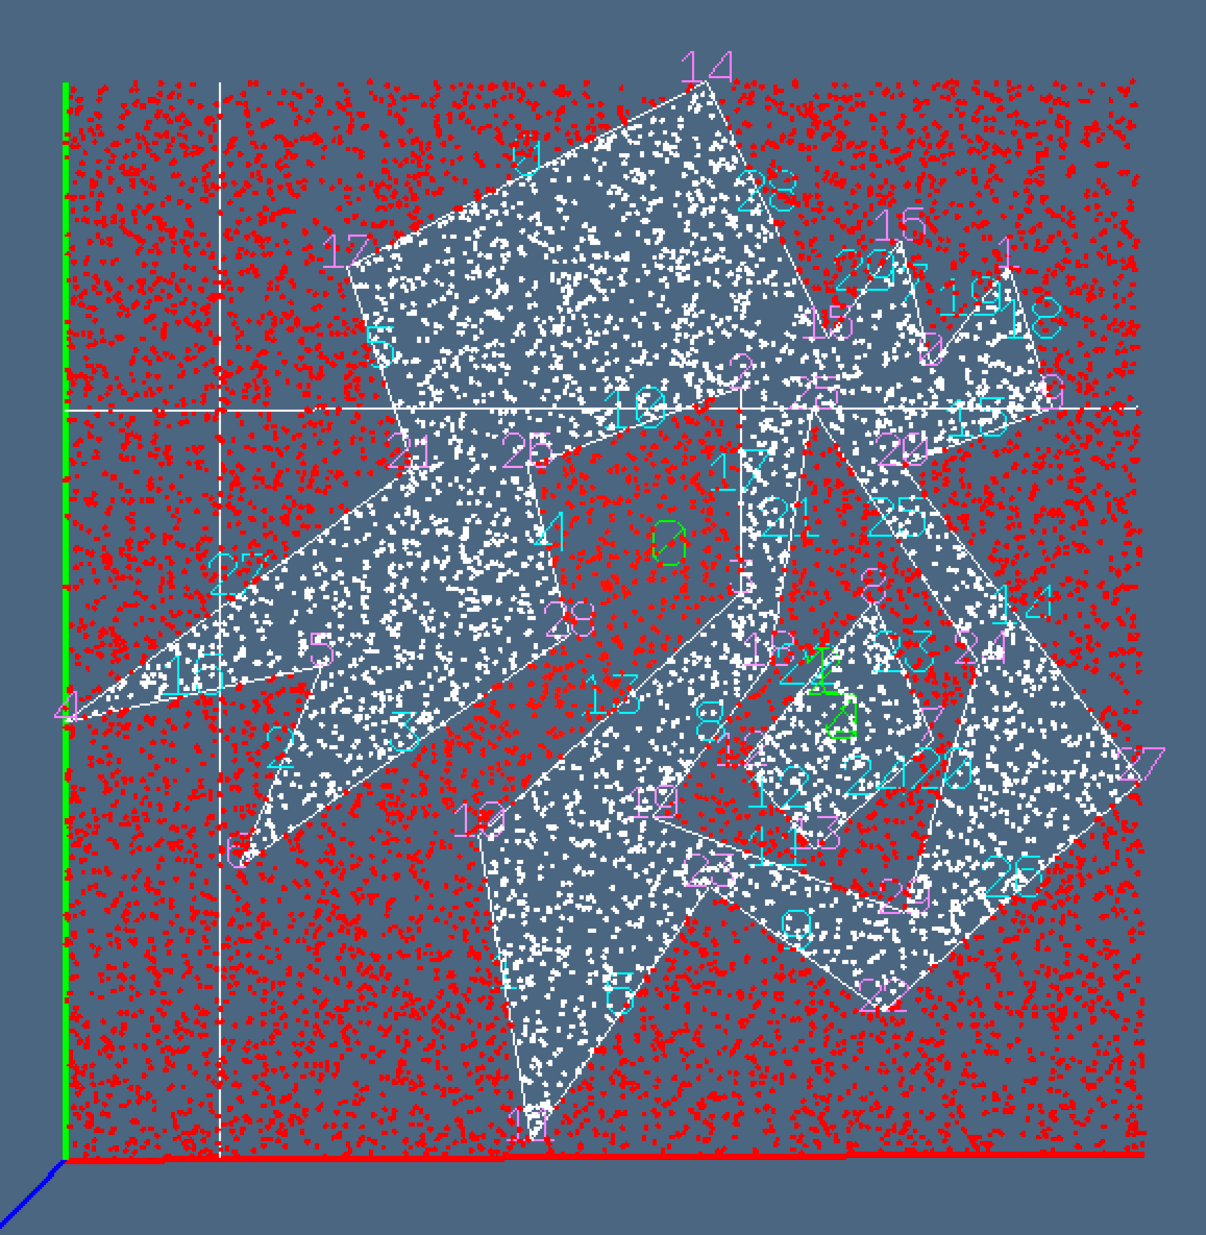
\includegraphics[width=0.5\linewidth]{images/pointInPolygon} 
   \caption{Testing the point-in-polygon algorithm.}
   \label{fig:pointInPolygon}
\end{figure}


\paragraph{Testing of point-in-polygon classification on a random polygon}

%-------------------------------------------------------------------------------
@O test/py/bool/test14.py @{
""" Testing of point-in-polygon classification  on a random polygon """
from larlib import *

filename = "test/svg/inters/tile.svg"
lines = svg2lines(filename)
V,EV = lines2lar(lines)

@< Point in polygon testing @>

result = []
classify = pointInPolygonClassification((V,EV))
for k in range(10000):
    queryPoint = [random.random(),random.random()]
    inOut = classify(queryPoint)
    #print k,queryPoint,inOut
    if inOut=="p_in": result += [MK(queryPoint)]
    elif inOut=="p_out": result += [COLOR(RED)(MK(queryPoint))]

VIEW(STRUCT(MKPOLS((V,EV))+result))
@}
%-------------------------------------------------------------------------------

\begin{figure}[htbp] %  figure placement: here, top, bottom, or page
   \centering
   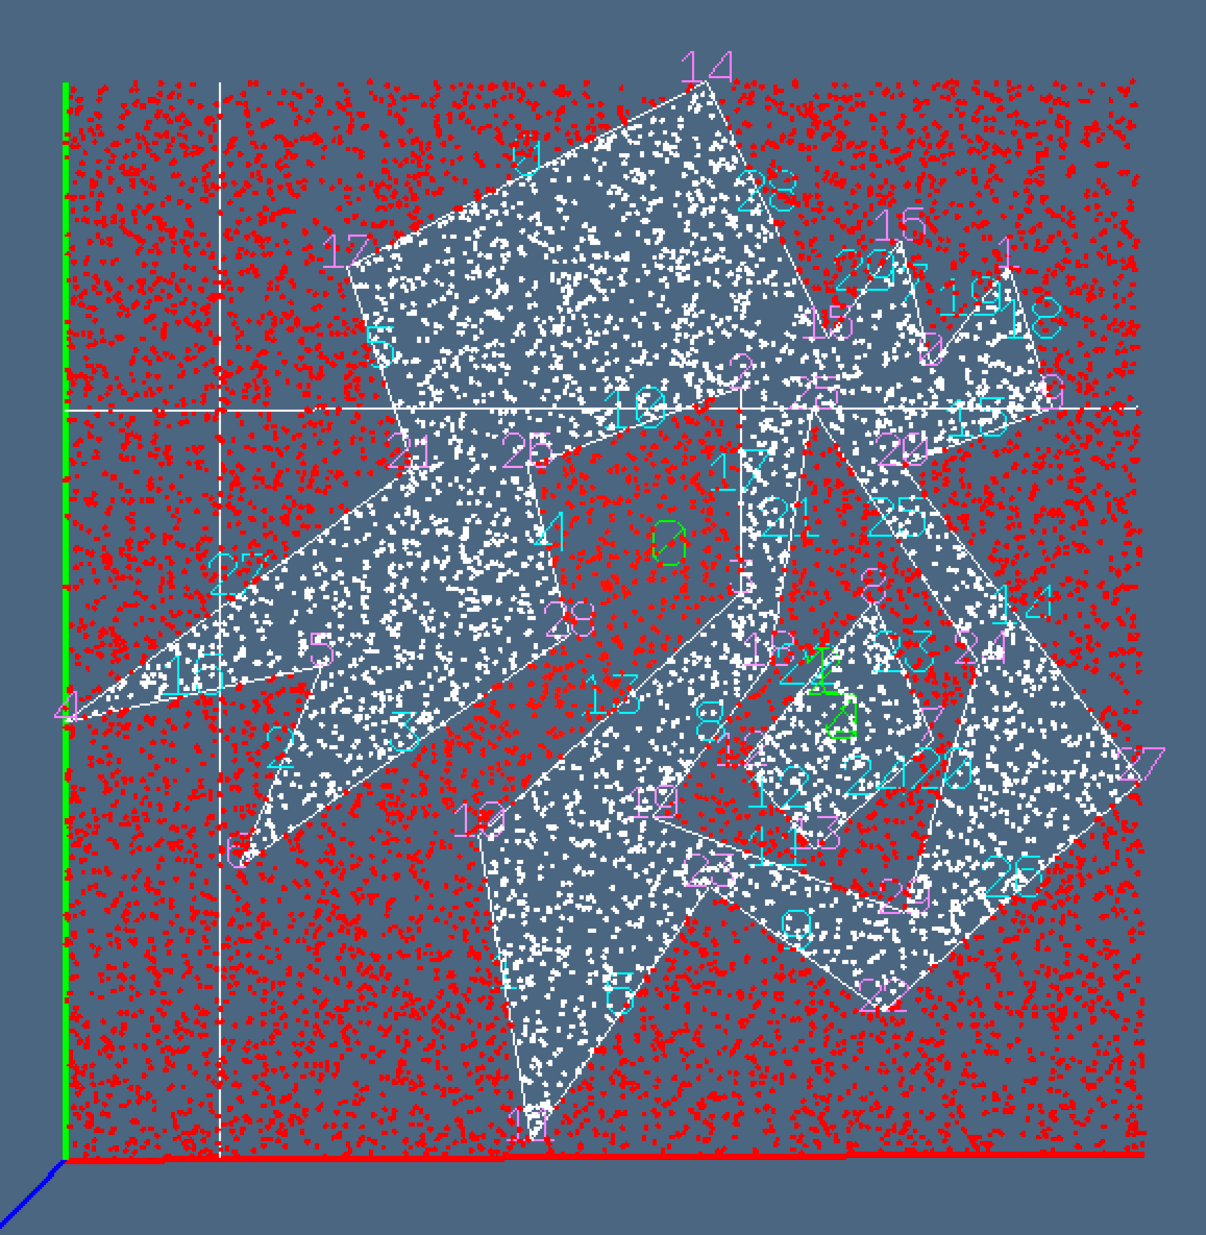
\includegraphics[width=0.5\linewidth]{images/pointInPolygon} 
   \caption{Testing the point-in-polygon algorithm.}
   \label{fig:pointInPolygon}
\end{figure}


\section{Exporting the library}
%===============================================================================

%-------------------------------------------------------------------------------
@O larlib/larlib/triangulation.py
@{""" Module for pipelined intersection of geometric objects """
from larlib import *
import inters

@< Return a feasible pair edge/vertex @>
@< Extract a single edge/vertex cycle @>
@< Extract all cycles from a LAR pair model @>
@< Edge cycles associated to a closed chain of edges @>
@< Point in polygon testing @>
@< Classification of non intersecting cycles @>
@< Extraction of path-connected boundaries @>
@< Transforming to polar coordinates @>
@< Scan line algorithm @>
@< Scan line algorithm input/output @>
@< Orientation of component cycles of unconnected boundaries @>
@< General composition of nested and non manifold cycles @>
@< From nested boundary cycles to triangulation @>
@< Generation of 1-boundaries as vertex permutation @>
@< Wire-frame LAR to boundary polygons @>
@< From Struct object to LAR boundary model @>
@< From structures to boundary polylines @>
@< From LAR boundary model to polylines @>
@< Computing a LAR 2-complex from an arrangement of line segments @>
@< Visualization of a 2D complex and 2-chain @>
@< Solid PyPLaSM visualization of a 2-complex @>
@}
%-------------------------------------------------------------------------------


\section{Testing }
%===============================================================================

This section in subdivided in two subsections, testing respectively (a) the construction and visualization of the containment lattice of non-intersecting polygonal cycles, and (b) the triangulation of the boundary polygon of random polygonal domains, including non connected parts, nested cycles and non-manifold cycles, both internal and external to the given 2D domain.

\subsection{Drawing multiply-connected boundary polylines}

A multiply-connected boundary polyline gives the boundary edges of a 2-cell.
In LAR, 2-cells must be connected, but not necessarily simply-connected (or path-connected, or homotopic to a point). The ``solid'' drawing of such a generally non-convex 2-cells is not easy.
In particular, they must be decomposed into a coherently-oriented simplicial 2-complex, i.e.~into a set of equioriented triangles. The library function used at this purpose (), contained in the \texttt{poly2tria} module, only accepts a single boundary polyline. Hence the purpose of this section is to transform a list of cycles, corresponding orderly to the exterior and the interior boundaries of a 2-cell, into a single polyline, using the so-called \emph{bridge-edges}~\cite{Yamaguchi:85} mechanism. The transformation from a set of non-intersecting boundary cycles to a single connected polyline is given in Section~\ref{sec:singlepolyline}.


\paragraph{Generating the LAR of a set of non-intersecting cycle}

We use the \texttt{test/svg/lattice.svg} file to test the exporting of different boundary chains. The example \texttt{test15.py} aims to prepare the computational environment for writing down the LAR of the 2-complex generated by any set of non-intersecting 1-cles in 2D.

Let us remenber that any $d$-cell in the domain of the LAR scheme must be connected, but not necessarily contractible to a point, i.e.~may contain internal holes.
The goal af this test and of the previous one, is hence to generalize the creation of 2-complexes (sets of polygons) starting from several non-intersecting boundary cycles, instead than starting from just one closed polyline.

The motivation arises from situations created by the Boolean algorithm, as well as from the imput of a 2-complex from general wire-frame drawings.

%-------------------------------------------------------------------------------
@O test/py/triangulation/test01.py
@{""" Testing containments between non intersecting cycles """
from larlib import *

filename = "test/svg/inters/facade.svg"
lines = svg2lines(filename)
VIEW(STRUCT(AA(POLYLINE)(lines)))

V,EV = lines2lar(lines)
V,EVs = biconnectedComponent((V,EV))
# candidate face
FVs = AA(COMP([list,set,CAT]))(EVs)

latticeArray = computeCycleLattice(V,EVs)

for k in range(len(latticeArray)):
   print k,latticeArray[k]

VV = AA(LIST)(range(len(V)))
submodel = STRUCT(MKPOLS((V,EV)))
VIEW(larModelNumbering(1,1,1)(V,[VV,EV,FVs],submodel,0.15)) 
@}
%-------------------------------------------------------------------------------


%-------------------------------------------------------------------------------
@O test/py/triangulation/test02.py
@{""" Generating the LAR of a set of non-intersecting cycles """
from larlib import *

sys.path.insert(0, 'test/py/triangulation/')
from test01 import *

cells = cellsFromCycles(latticeArray)
CV = AA(COMP([list,set,CAT]))(EVs)
EVdict = dict(zip(EV,range(len(EV))))
FE = [[EVdict[edge] for edge in cycle] for cycle in EVs] 
edges = [CAT([FE[cycle] for cycle in cell]) for cell in cells]
FVs = [[CV[cycle] for cycle in cell] for cell in cells]
FV = AA(CAT)(FVs)
cycles = STRUCT(MKPOLS((V,EV)))
csrBoundaryMat = boundary(FV,EV)

n = len(cells)
chains = allBinarySubsetsOfLenght(n)
for chain in chains:
    chainBoundary = COLOR(RED)(STRUCT(MKPOLS((V,[EV[e] 
                        for e in chain2BoundaryChain(csrBoundaryMat)(chain)]))))
    VIEW(STRUCT([cycles, chainBoundary]))
@}
%-------------------------------------------------------------------------------


\paragraph{LAR of the 2-complex generated by non-intersecting cycles}

Therefore, the LAR of the 2-complex generated from the input get from \texttt{test15.py}
is \texttt{(V,FV,EV)} with the components given by the the following:

\begin{verbatim}
V = [[0.7808,0.6751],[0.6044,0.6751],[0.319,0.5804],[0.319,0.3994],[0.8936,0.0],
[0.0,0.0],[0.6044,0.8123],[0.7808,0.8123],[0.3495,0.6751],[0.3495,0.8123],
[0.1218,0.3036],[0.2983,0.3036],[0.0886,0.3994],[0.0886,0.5804],[0.2581,0.4505],
[0.1495,0.4505],[0.7717,0.4213],[0.5952,0.4213],[0.7717,0.5585],[0.0,1.0],
[0.3403,0.1664],[0.3403,0.3036],[0.5952,0.5585],[0.5168,0.1664],[0.5168,0.3036],
[0.5259,0.8123],[0.1495,0.5293],[0.5259,0.6751],[0.8936,1.0],[0.2983,0.1664],
[0.1218,0.1664],[0.2581,0.5293],[0.4965,0.7815],[0.4965,0.7059],[0.2983,
0.5585],[0.2983,0.4213],[0.1218,0.4213],[0.3789,0.7815],[0.1218,0.5585],
[0.3789,0.7059]]
\end{verbatim}

\begin{verbatim}
FV = [[0,1,2,3,4,5,6,7,8,9,10,11,12,13,16,17,18,19,20,21,22,23,24,25,27,
28,29,30],[32,33,37,39],[34,35,36,38,26,15,14,31]]
\end{verbatim}

\begin{verbatim}
EV = [(0,1),(0,7),(1,6),(2,3),(2,13),(3,12),(4,5),(4,28),(5,19),(6,7),(8,9),
(8,27),(9,25),(10,11),(10,30),(11,29),(12,13),(14,15),(14,31),(15,26),
(16,17),(16,18),(17,22),(18,22),(19,28),(20,21),(20,23),(21,24),(23,24),
(25,27),(26,31),(29,30),(32,33),(32,37),(33,39),(34,35),(34,38),(35,36),
(36,38),(37,39)]
\end{verbatim}

Of course, this LAR representation gives full control of the complex topology, including $k$-(co)chains and (co)boundary operators. For example, in Figure~\ref{fig:cycles} we show a solid image of the three 2-cells in \texttt{FV}, and, drawn in red the boundary 1-cells in the complex, corresponding to the 2-chains of coordinates $[1,0,0]$,  $[0,1,0]$, $[0,0,1]$, and $[1,1,0]$, respectively.


\begin{figure}[htbp] %  figure placement: here, top, bottom, or page
   \centering
   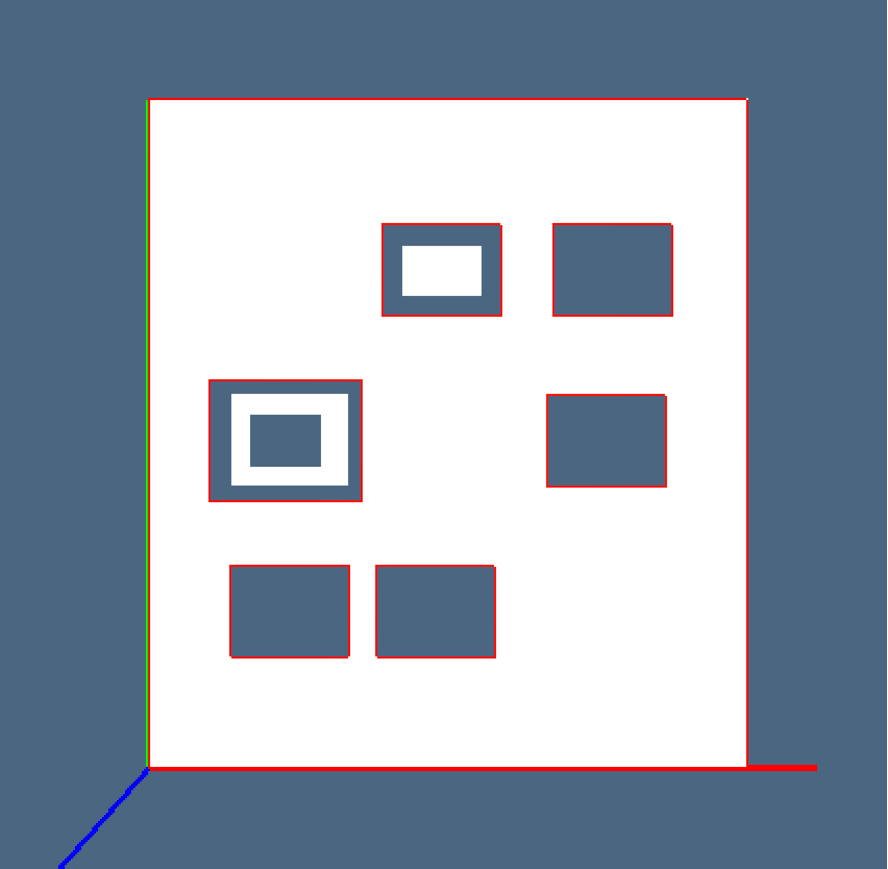
\includegraphics[height=0.24\linewidth,width=0.24\linewidth]{images/cycles1}
   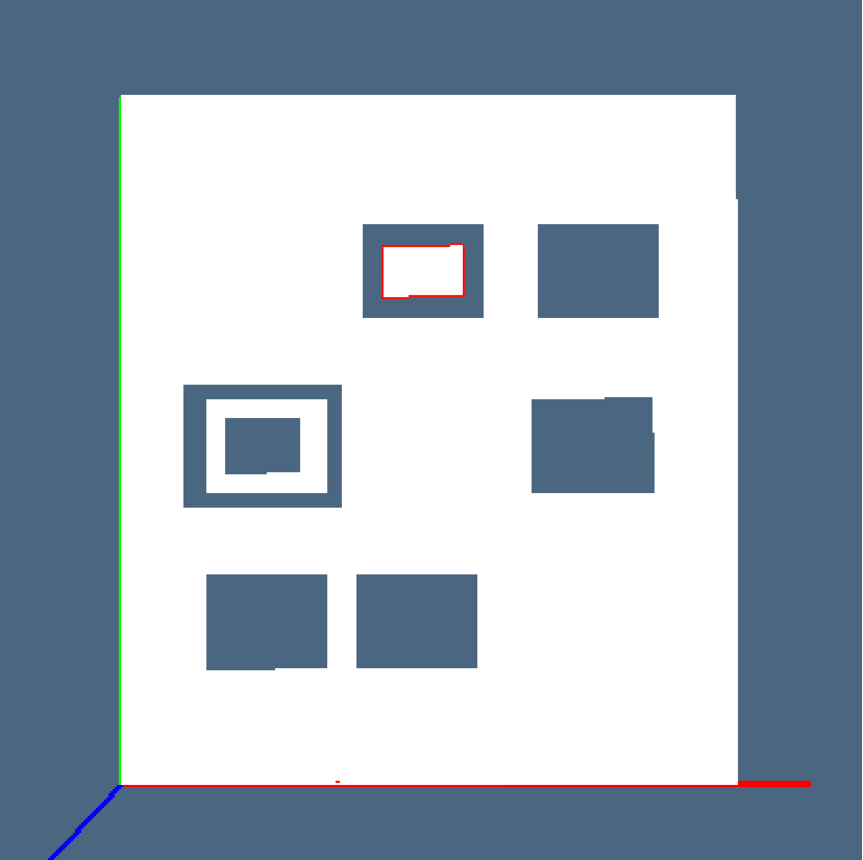
\includegraphics[height=0.24\linewidth,width=0.24\linewidth]{images/cycles2} 
   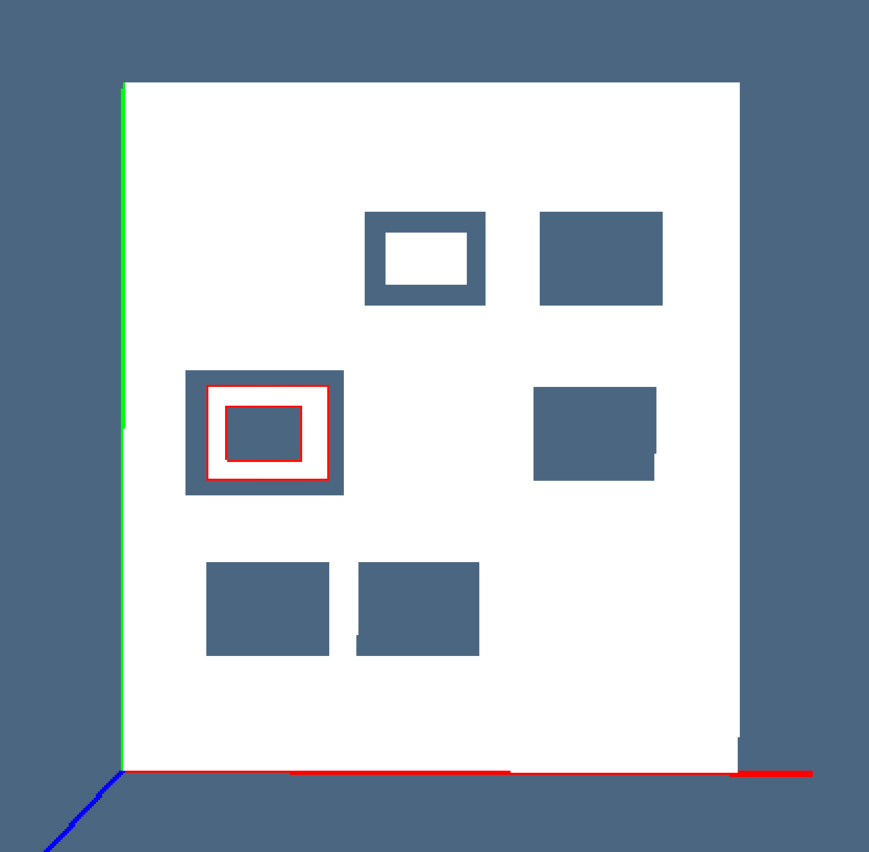
\includegraphics[height=0.24\linewidth,width=0.24\linewidth]{images/cycles3} 
   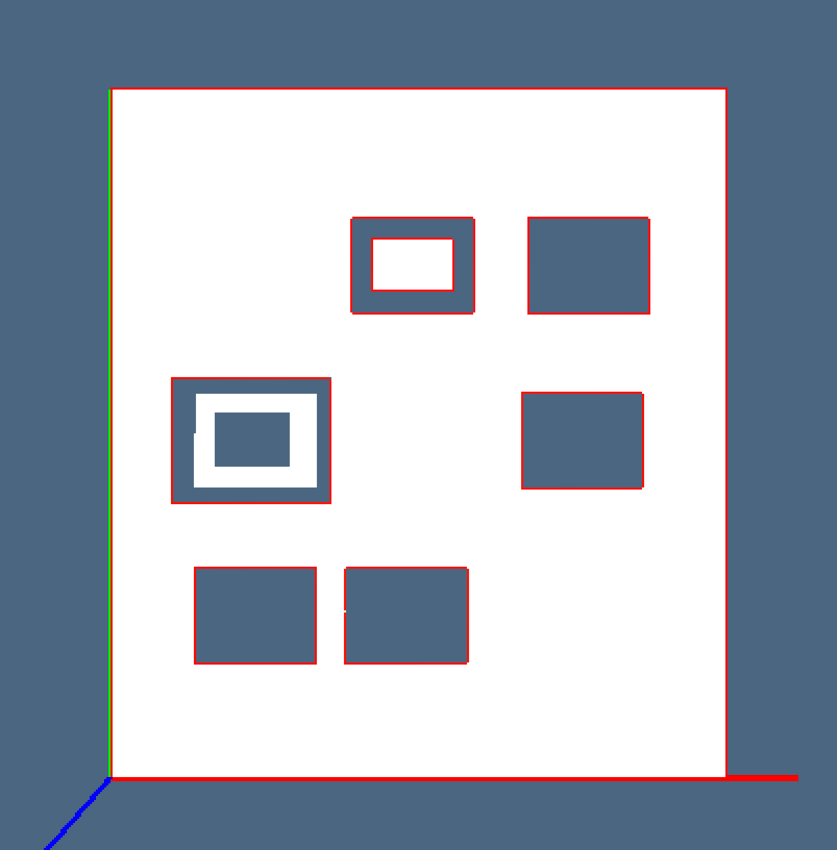
\includegraphics[height=0.24\linewidth,width=0.24\linewidth]{images/cycles4} 
   \caption{Some examples of boundaries (in red) of 2-chains from nested non intersecting cycles.}
   \label{fig:cycles}
\end{figure}


\subsection{Boundary polylines}

\paragraph{Generating the LAR of a set of non-intersecting cycles}
The example provided by \texttt{test/py/inters/test17.py} is completed here
by showing the solid drawing of the generated LAR data structure, and superimposing to it 
the boundary 1-chains generated by several 2-chains.

%-------------------------------------------------------------------------------
@O test/py/triangulation/test03.py
@{""" Generating the LAR of a set of non-intersecting cycles """
from larlib import *

sys.path.insert(0, 'test/py/triangulation/')
from test02 import *

lar = (V,FV,EV)

bcycles,_ = boundaryCycles(range(len(EV)),EV)
polylines = [[V[EV[e][1]] if e>0 else V[EV[-e][0]] for e in cycle ] for cycle in bcycles]
polygons = [polyline + [polyline[0]] for polyline in polylines]

complex = SOLIDIFY(STRUCT(AA(POLYLINE)(polygons)))
csrBoundaryMat = boundary(FV,EV)

for chain in chains:
    chainBoundary = COLOR(RED)(STRUCT(MKPOLS((V,[EV[e] 
                        for e in chain2BoundaryChain(csrBoundaryMat)(chain)]))))
    VIEW(STRUCT([complex, chainBoundary]))
@}
%-------------------------------------------------------------------------------

%-------------------------------------------------------------------------------
@O test/py/triangulation/test04.py
@{""" Orienting a set of non-intersecting cycles """
from larlib import *

sys.path.insert(0, 'test/py/triangulation/')
from test03 import *

cells,bridgeEdges = connectTheDots((V,EV))
CVs = orientBoundaryCycles((V,EV),cells)
@}
%-------------------------------------------------------------------------------

%-------------------------------------------------------------------------------
@O test/py/triangulation/test05.py
@{""" Generating the LAR of a set of non-intersecting cycles """
from larlib import *

sys.path.insert(0, 'test/py/triangulation/')
from test03 import *

W,EW = boundaryCycles2vertexPermutation( (V,EV) )
VIEW(EXPLODE(1.2,1.2,1.2)(MKPOLS((W,EW))))
@}
%-------------------------------------------------------------------------------

%-------------------------------------------------------------------------------
@O test/py/triangulation/test06.py
@{""" Generating the Triangulation of a set of non-intersecting cycles """
from larlib import *

sys.path.insert(0, 'test/py/triangulation/')
from test03 import *

triangleSet = larTriangulation( (V,EV) )

VIEW(STRUCT(AA(JOIN)(AA(AA(MK))(CAT(triangleSet)))))
VIEW(SKEL_1(STRUCT(AA(JOIN)(AA(AA(MK))(CAT(triangleSet))))))

"""
model = V,EV
W,FW = lar2boundaryPolygons(model)
polygons = [[W[u] for u in poly] for poly in FW]
VIEW(STRUCT(AA(POLYLINE)(polygons)))

triangleSet,triangledFace = [],[]
for polygon in polygons:  
    triangledPolygon = []
    polyline = []
    for p in polygon:
        polyline.append(Point(p[0],p[1]))
    cdt = CDT(polyline)

    triangles = cdt.triangulate()
    trias = [ [[t.a.x,t.a.y,0],[t.c.x,t.c.y,0],[t.b.x,t.b.y,0]] for t in triangles ]
    triangleSet += [AA(REVERSE)(trias)]
"""
@}
%-------------------------------------------------------------------------------



\subsection{Testing with random polygons}
%===============================================================================

In order to test the algorithms implemented in this library, we make use of random triangulations of $C_2=\{x\in\R^2: \norm{x}\leq 1\}$.

\begin{figure}[htbp] %  figure placement: here, top, bottom, or page
   \centering
   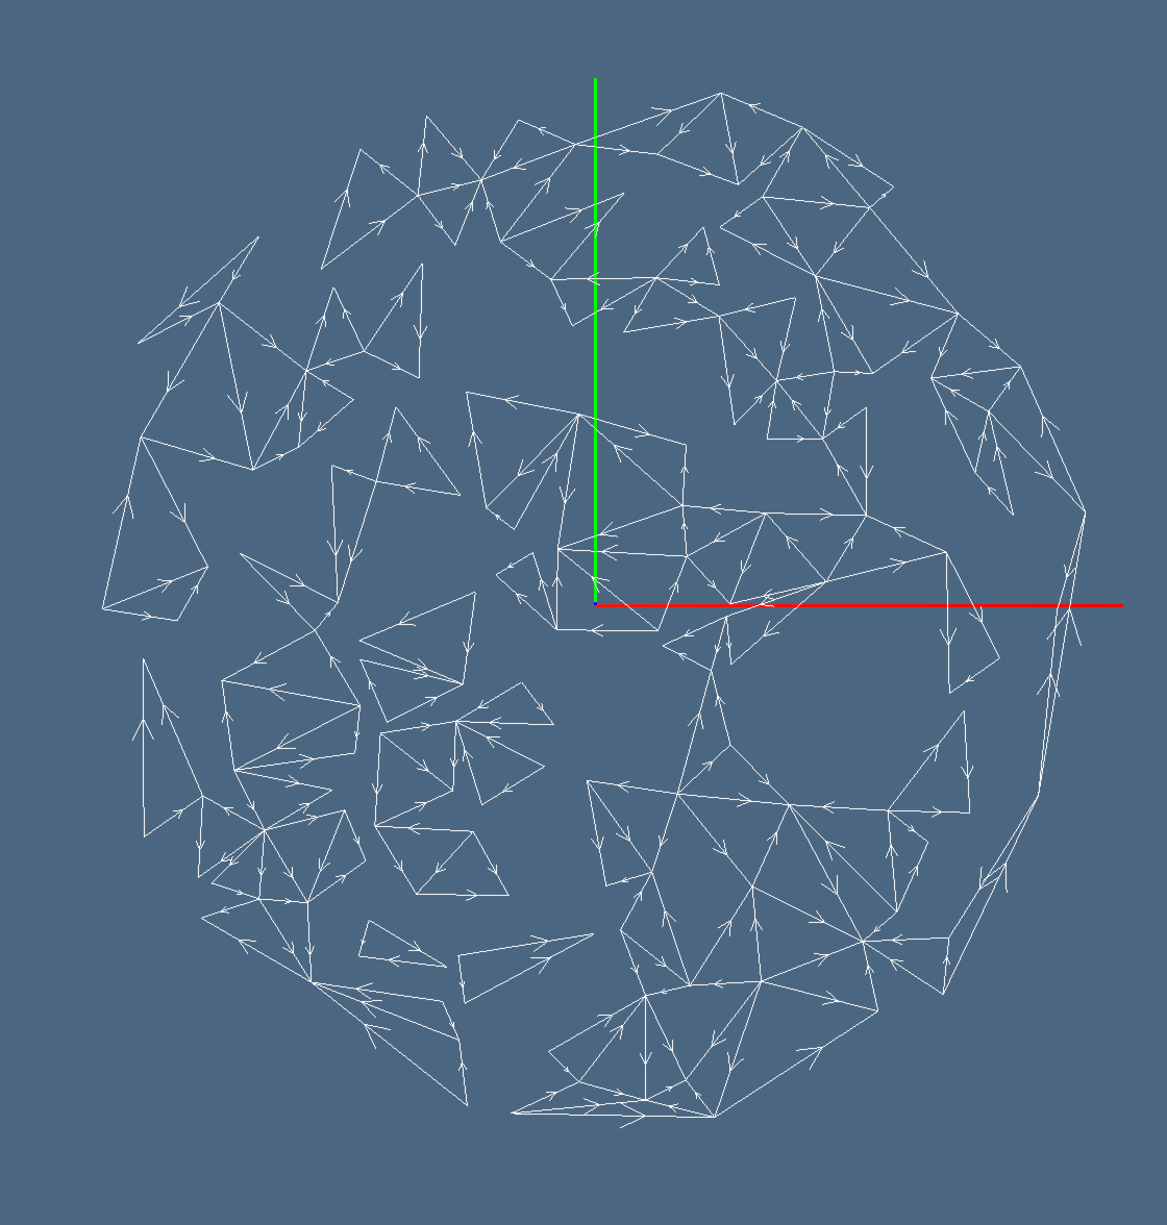
\includegraphics[width=0.33\linewidth]{images/alg-tria0} 
   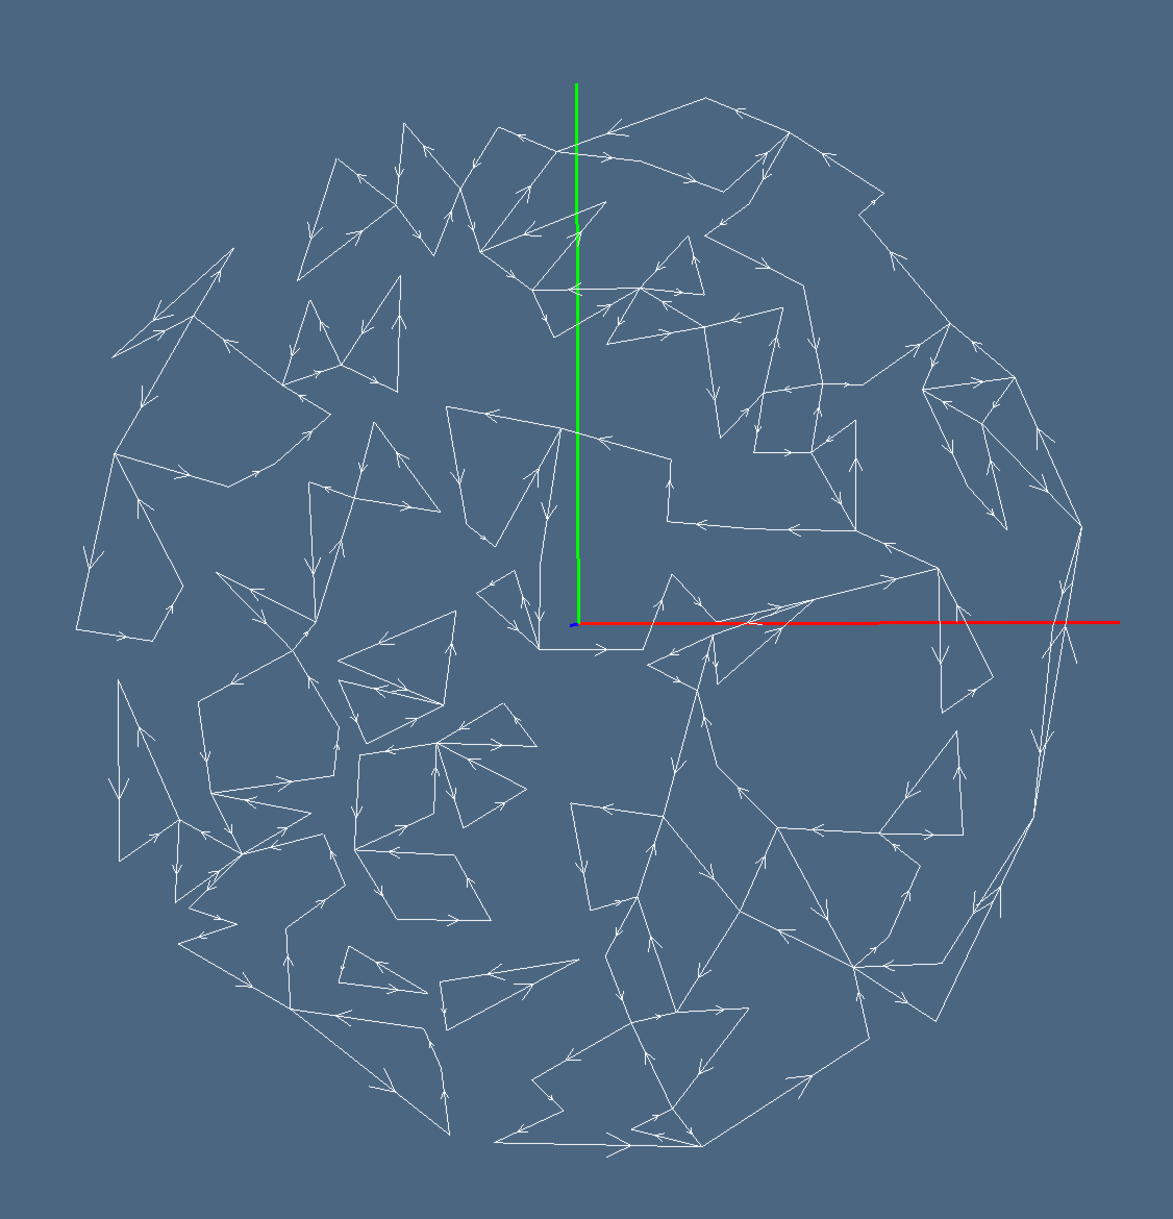
\includegraphics[width=0.33\linewidth]{images/alg-tria1} 
   \caption{example caption}
   \label{fig:example}
\end{figure}

%-------------------------------------------------------------------------------
@O test/py/triangulation/test07.py
@{
from larlib import *

@< random 1-boundary generation @>
@}
%-------------------------------------------------------------------------------

\paragraph{random 1-boundary generation}

%-------------------------------------------------------------------------------
@D random 1-boundary generation
@{""" random 1-boundary generation """
from larlib import *

import sys
sys.path.insert(0, '/Users/paoluzzi/Documents/dev/lar-cc/test/py/larcc/')
from test16 import *

EV = AA(list)(cells)
V,polygons,EV = larPair2Triple((V,EV))
FV = AA(list)(AA(set)(AA(CAT)(polygons)))

bcycles,bverts = boundaryCycles(range(len(EV)),EV)
VIEW(STRUCT(AA(POLYLINE)([[V[v] for v in verts+[verts[0]]] for verts in bverts])))

colors = [CYAN,MAGENTA,WHITE,RED,YELLOW,GRAY,GREEN,ORANGE,BLUE,PURPLE,BROWN,BLACK]
components = [COLOR(colors[k%12])(face) for k,face in enumerate(MKFACES((V,FV,EV)))]
VIEW(STRUCT(components))
@}
%-------------------------------------------------------------------------------






\bibliographystyle{amsalpha}
\bibliography{triangulation}

\end{document}
